\documentclass[11pt]{article}

\usepackage{macros}

\title{Course Notes for EE227C (Spring 2018):\\
 Convex Optimization and Approximation }
\author{Instructor: Moritz Hardt\\
{\small Email: \tt hardt+ee227c@berkeley.edu}\\ ~\\
Graduate Instructor: Max Simchowitz\\
{\small Email: \tt msimchow+ee227c@berkeley.edu}\\ ~\\
}


\begin{document}

\maketitle

\begin{abstract}
This course explores some theory and algorithms for nonlinear optimization. We
will focus on problems that arise in machine learning and modern data analysis,
paying attention to concerns about complexity, robustness, and implementation in
these domains. We will also see how tools from convex optimization can help
tackle non-convex optimization problems common in practice.

Code examples are available at:

\begin{center}
{\Large \url{https://ee227c.github.io/}.}
\end{center}

Below are the course notes for EE227C (Spring 2018): Convex Optimization and
Approximation, taught at UC Berkeley. 
\end{abstract}


\pagebreak

\setcounter{tocdepth}{2}
\tableofcontents

\pagebreak

\part{Gradient methods}
\section{Lecture 1: Convexity}
\sectionlabel{convexity}

This lecture provides the most important facts about convex sets and convex
functions that we'll heavily make use of. These are often simple consequences of
Taylor's theorem.

\subsection{Convex sets}

\begin{definition}[Convex set]
A set $K\subseteq\R^n$ is \emph{convex} if it the line segment between any two points in~$K$ is also contained in~$K.$ Formally, for all $x,y\in K$ and all scalars $\gamma\in[0,1]$ we have $\gamma x+(1-\gamma)y\in K.$
\end{definition}

\begin{theorem}[Separation Theorem]
\theoremlabel{separation}
Let $C, K\subseteq\R^n$ be convex sets with empty intersection $C\cap K=\emptyset.$ Then there exists a point $a\in\R^n$ and a number $b\in\R$ such that
\begin{enumerate}
\item for all $x\in C,$ we have $\langle a, x\rangle \ge b.$
\item for all $x\in K,$ we have $\langle a, x\rangle \le b.$
\end{enumerate}
If $C$ and $K$ are closed and at least one of them is bounded, then we can replace the inequalities by strict inequalities.
\end{theorem}
The case we're most concerned with is when both sets are compact (i.e., closed and bounded). We highlight its proof here.
\begin{proof}[Proof of \theoremref{separation} for compact sets.]
In this case, the Cartesian product $C\times K$ is also compact. Therefore, the
distance function $\|x-y\|$ attains its minimum over $C\times K.$ Taking $p, q$
to be two points that achieve the minimum. A separating hyperplane is given by
the hyperplane perpendicular to $q-p$ that passes through the midpoint between
$p$ and $q.$ That is, $a=q-p$ and $b=(\langle a, q\rangle - \langle a,
p\rangle)/2.$ For the sake of contradiction, suppose there is a point~$r$ on
this hyperplane contained in one of the two sets, say,~$C.$ Then the line
segment from $p$ to $r$ is also contained in~$C$ by convexity. We can then find
a point along the line segment that is close to $q$ than $p$ is, thus
contradicting our assumption.
\end{proof}

\subsubsection{Notable convex sets}
\begin{itemize}
\item Linear spaces $\{x\in\R^n\mid Ax=0\}$ and halfspaces $\{x\in\R^n \mid \langle a, x\rangle \ge 0 \}$
\item Affine transformations of convex sets. If $K\subseteq\R^n$ is convex, so is $\{Ax+b\mid x\in K\}$ for any $A\in\R^{m\times n}$ and $b\in\R^m.$
In particular, affine subspaces and affine halfspaces are convex.
\item Intersections of convex sets. In fact, every convex set is equivalent to the intersection of all affine halfspaces that contain it (a consequence of the separating hyperplane theorem).
\item The cone of positive semidefinite matrices, denotes, $S^n_+ = \{ A\in\R^{n\times n}\mid A\succeq 0\}.$ Here we write $A\succeq 0$ to indicate that $x^\trans A x\ge 0$ for all $x\in\R^n.$ The fact that $S^n_+$ is convex can be verified directly from the definition, but it also follows from what we already knew. 
Indeed, denoting by $S_n=\{A\in\R^{n\times n}\mid A^\trans = A\}$ the set of all $n\times n$ symmetric matrices, we can write $S^n_+$ as an (infinite) intersection of halfspaces $S^n_+=\bigcap_{x\in\R^n\backslash\{0\}} \{ A\in S_n\mid x^\trans A x\ge 0\}.$
\item See Boyd-Vandenberghe for lots of other examples.
\end{itemize}

\subsection{Convex functions}

\begin{definition}[Convex function]
A function $f\colon\domain\to\R$ is \emph{convex} if for all $x,y\in\domain$ and all scalars $\gamma\in[0,1]$ we have $f(\gamma x+(1-\gamma)y)\le \gamma f(x)+(1-\gamma)f(y).$
\end{definition}

Jensen (1905) showed that for continuous functions, convexity follows from the ``midpoint'' condition that for all $x,y\in\domain,$
\[
f\left(\frac{x+y}2\right)\le \frac{f(x)+f(y)}2\,.
\]
This result sometimes simplifies the proof that a function is convex in cases where we already know that it's continuous.

\begin{figure}
\begin{center}
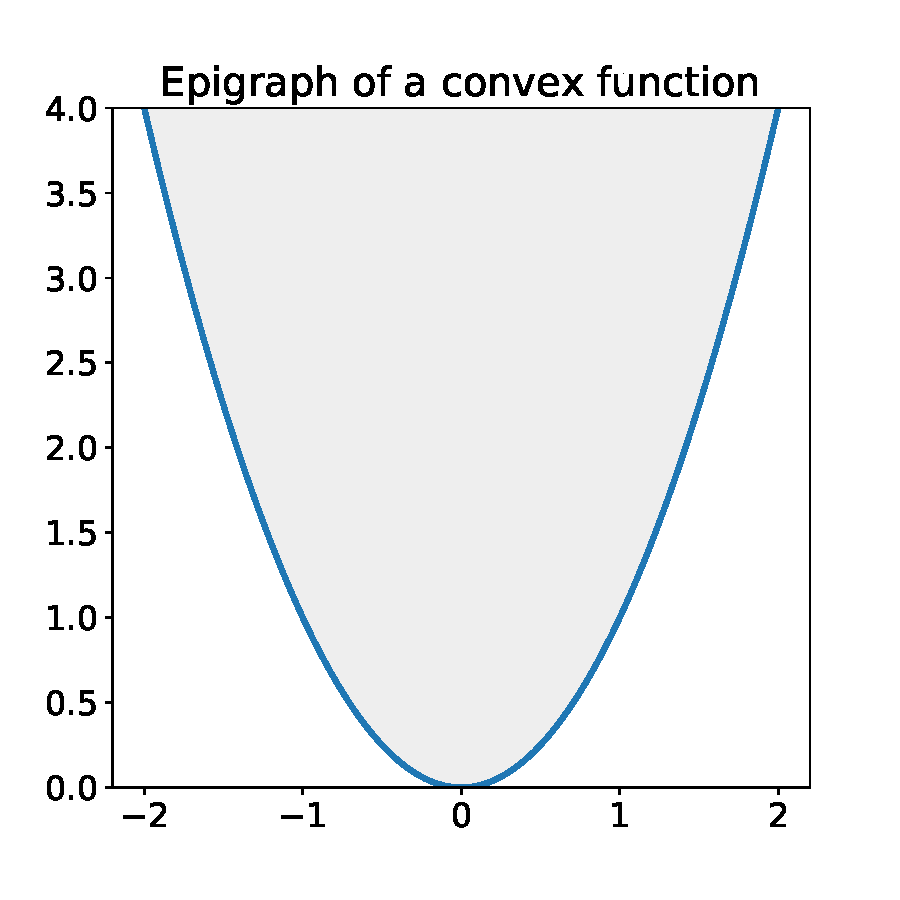
\includegraphics[width=3in]{figures/lecture1-epigraph}
\end{center}
\end{figure}
\begin{definition}

The \emph{epigraph} of a function~$f\colon \domain\to\R$ is defined as 
\[
\epi(f) = \{(x, t)\mid f(x)\le t\}\,.
\]
\end{definition}

\begin{fact}
A function is convex if and only if its epigraph is convex.
\end{fact}

Convex functions enjoy the property that local minima are also global minima. Indeed, suppose that $x\in\domain$ is a local minimum of~$f\colon\domain\to\R$ meaning that any point in a neighborhood around $x$ has larger function value. Now, for every $y\in\domain,$ we can find a small enough $\gamma$ such that
\[
f(x) \le f((1-\gamma)x+\gamma y) \le (1-\gamma)f(x)+\gamma f(y)\,.
\]
Therefore, $f(x)\le f(y)$ and so $x$ must be a global minimum.

\subsubsection{First-order characterization}

It is helpful to relate convexity to Taylor's theorem, which we recall now. We define the \emph{gradient} of a differentiable function~$f\colon\domain\to\R$ at $x\in\domain$ as the vector of partial derivatives
\[
\nabla f(x) = \left( \frac{\partial f}{\partial x_i} \right)_{i=1}^n\,.
\]
We note the following simple fact that relates linear forms of the gradient to a
one-dimensional derivative evaluated at~$0.$ It's a consequence of the multivariate chain rule.
\begin{fact}
\factlabel{1d-nd-gradient}
Assume $f\colon\domain\to\R$ is differentiable and let $x,y\in\domain.$ Then,
\[
\nabla f(x)^\trans y
= \left.\frac{\partial f(x+\gamma y)}{\partial \gamma}\right|_{\gamma=0}\,.
\]
\end{fact}
Taylor's theorem implies the following statement.
\begin{proposition}
\propositionlabel{first-order-taylor}
Assume $f\colon\domain\to\R$ is continuously differentiable along the line segment between two points $x$ and $y.$ Then,
\[
f(y) = f(x) 
+ \nabla f(x)^\trans (y-x)
+ \int_0^1 (1-\gamma)\frac{\partial^2 f(x+\gamma(y-x))}{\partial\gamma^2}\rd\gamma
\]
\end{proposition}
\begin{proof}
Apply a second order Taylor's expansion to $g(\gamma)=f(x+\gamma(y-x))$ and apply \factref{1d-nd-gradient} to the first-order term. 
\end{proof}

Among differentiable functions, convexity is equivalent to the property that the first-order Taylor approximation provides a global lower bound on the function.

\begin{figure}
\begin{center}
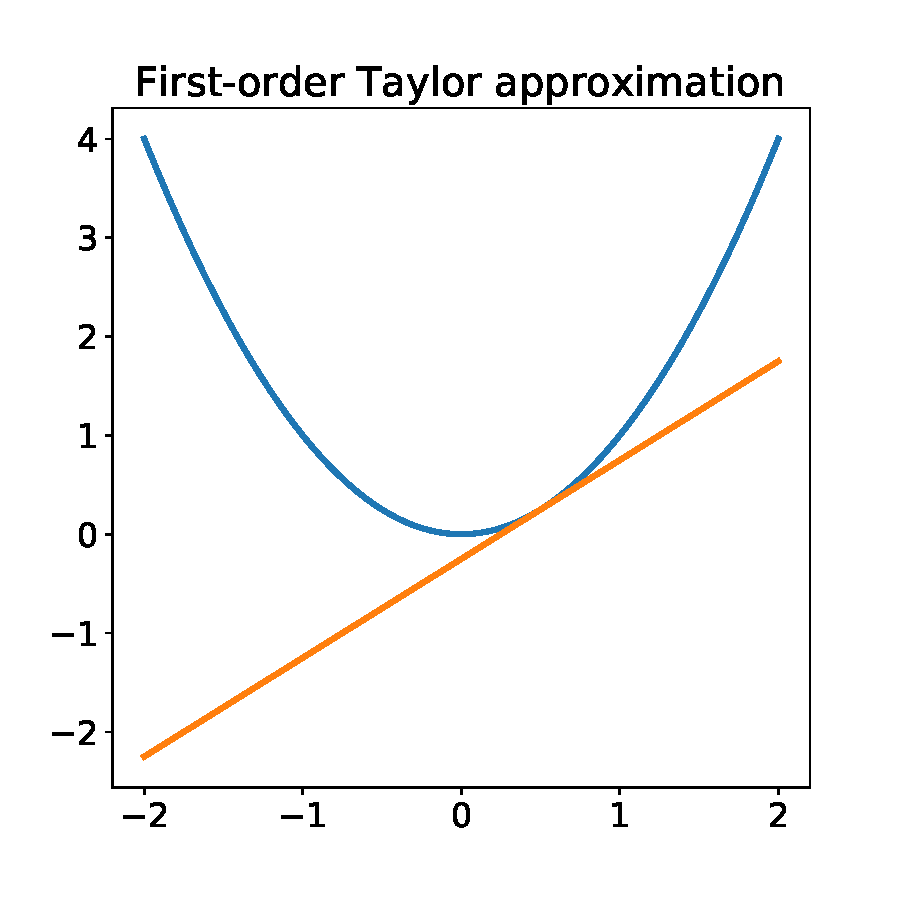
\includegraphics[width=3in]{figures/lecture1-taylor}
\end{center}
\caption{Taylor approximation of $f(x)=x^2$ at $0.5.$}
\end{figure}

\begin{proposition}
\propositionlabel{first-order-lower-bound}
Assume $f\colon\domain\to\R$ is differentiable. Then, $f$ is convex if and only if for all $x,y\in\domain$ we have
\begin{equation}\equationlabel{first-order-lower-bound}
f(y) \ge f(x) + \nabla f(x)^\trans (y-x)\,.
\end{equation}
\end{proposition}
\begin{proof}
First, suppose $f$ is convex, then by definition
\begin{align*}
f(y) &\ge \frac{f((1-\gamma)x+\gamma y)-(1-\gamma)f(x)}{\gamma}\\
&\ge f(x) +\frac{f(x+\gamma(y-x))-f(x)}\gamma\\
&\rightarrow f(x) +\nabla f(x)^\trans (y-x) \quad\text{as $\gamma\to 0$} \tag{by \factref{1d-nd-gradient}.}
\end{align*}
On the other hand, fix two points $x, y\in\domain$ and $\gamma\in[0,1]$. Putting $z=\gamma x + (1-\gamma)y$ we get from applying \equationref{first-order-lower-bound} twice,
\[
f(x) \ge f(z) + \nabla f(z)^\trans (x-z)
\quad\text{and}\quad
f(y) \ge f(z) + \nabla f(z)^\trans (y-z)
\]
Adding these inequalities scaled by $\gamma$ and $(1-\gamma)$, respectively, we get $\gamma f(x)+(1-\gamma)f(y)\ge f(z),$ which establishes convexity.
\end{proof}

A direct consequence of \propositionref{first-order-lower-bound} is that
if $\nabla f(x)=0$ vanishes at a point~$x,$ then $x$ must be a global minimizer
of~$f.$

\begin{remark}[Subgradients]
Of course, not all convex functions are differentiable. The absolute
value~$f(x)=|x|,$ for example, is convex but not differentiable at $0.$
Nonetheless, for every $x,$ we can find a vector $g$ such that
\[
f(y) \ge f(x) + g^\trans (y-x)\,.
\]
Such a vector is called a \emph{subgradient} of $f$ at $x.$ The existence of
subgradients is often sufficient for optimization.
\end{remark}

\subsubsection{Second-order characterization}

We define the \emph{Hessian} matrix of $f\colon\domain\to\R$ at a point $x\in\domain$ as the matrix of second order partial derivatives:
\[
\nabla^2 f(x) = \left( \frac{\partial^2 f}{\partial x_i\partial x_j} \right)_{i,j\in[n]}\,.
\]
Schwarz's theorem implies that the Hessian at a point $x$ is symmetric provided
that $f$ has continuous second partial derivatives in an open set around~$x.$

In analogy with \factref{1d-nd-gradient}, we can relate quadratic forms in the
Hessian matrix to one-dimensional derivatives using the chain rule.
\begin{fact}
\factlabel{1d-nd-hessian}
Assume that $f\colon\domain\to\R$ is twice differentiable along the line segment from $x$ to $y.$ Then,
\[
y^\trans \nabla^2f(x+\gamma y)y 
= \frac{\partial^2f(x+\gamma y)}{\partial\gamma^2}\,.
\]
\end{fact}

\begin{proposition}
If $f$ is twice continuously differentiable on its domain~$\domain$, then $f$ is convex if and only if $\nabla^2 f(x)\succeq 0$ for all $x\in\domain.$ 
\end{proposition}
\begin{proof}
Suppose $f$ is convex and our goal is to show that the Hessian is positive semidefinite. 
Let $y=x + \alpha u$ for some arbitrary vector~$u$ and scalar $\alpha.$
\propositionref{first-order-lower-bound} shows
\[
f(y) - f(x) -\nabla f(x)^\trans (y-x) \ge 0
\]
Hence, by \propositionref{first-order-taylor},
\begin{align*}
0&\le  \int_0^1 (1-\gamma)\frac{\partial^2 f(x+\gamma(y-x))}{\partial\gamma^2}\rd\gamma\\
&=  (1-\gamma)\frac{\partial^2 f(x+\gamma(y-x))}{\partial\gamma^2}
\quad\text{for some $\gamma\in(0,1)$} \tag{by the mean value theorem}\\
&= (1-\gamma)(y-x)^\trans \nabla^2 f(x+\gamma (y-x))(y-x) 
\tag{by \factref{1d-nd-hessian}}\,.
\end{align*}
Plugging in our choice of~$y,$ this shows $0\le u^\trans \nabla^2
f(x+\alpha\gamma u)u.$ Letting $\alpha$ tend to zero establishes that $\nabla^2
f(x)\succeq 0.$ (Note that $\gamma$ generally depends on $\alpha$ but is always
bounded by~$1.$)

Now, suppose the Hessian is positive semidefinite everywhere in $\domain$ and
our goal is to show that  the function~$f$ is convex.  Using the same derivation
as above, we can see that the second-order error term in Taylor's theorem must
be nonnegative. Hence, the first-oder approximation is
a global lower bound and so the function~$f$ is convex by
\propositionref{first-order-lower-bound}.
\end{proof}

\subsection{Convex optimization}
Much of this course will be about different ways of minimizing a convex function~$f\colon\domain\to\R$ over a convex domain~$\domain:$ 
\[
\min_{x\in \Omega} f(x)
\]
Convex optimization is not necessarily easy! 
For starters, convex sets do not necessarily enjoy compact descriptions. When solving computational problems involving convex sets, we need to worry about how to represent the convex set we're dealing with. Rather than asking for an explicit description of the set, we can instead require a computational abstraction that highlights essential operations that we can carry out. The Separation Theorem motivates an important computational abstraction called \emph{separation oracle}.

\begin{definition}
A \emph{separation oracle} for a convex set~$K$ is a device, which given any point $x\not\in K$ returns a hyperplane separating $x$ from $K.$
\end{definition}

Another computational abstraction is a \emph{first-order oracle} that given a point $x\in\domain$ returns the gradient $\nabla f(x).$ Similarly, a \emph{second-order oracle} returns $\nabla^2 f(x).$ A function value oracle or \emph{zeroth-order oracle} only returns $f(x).$
First-order methods are algorithms that make do with a first-order oracle.

\subsubsection{What is efficient?}
Classical complexity theory typically quantifies the resource consumption (primarily running time or memory) of an algorithm in terms of the bit complexity of the input. 
This approach can be cumbersome in convex optimization and most textbooks shy away from it. 
Instead, it's customary in optimization to quantify the cost of the algorithm in terms of how often it accesses one of the oracles we mentioned.

The definition of ``efficient'' is not completely cut and dry in optimization. 
Typically, our goal is to show that an algorithm finds a solution~$x$ with $f(x) = \min_{x\in\domain}f(x) + \epsilon$ for some additive error $\epsilon>0.$ 
The cost of the algorithm will depend on the target error. 
Highly practical algorithms often have a polynomial dependence on $\epsilon,$ such as $O(1/\epsilon)$ or even $O(1/\epsilon^2).$ Other algorithms achieve $O(\log(1/\epsilon))$ steps in theory, but are prohibitive in their actual computational cost. Technically, if we think of the parameter~$\epsilon$ as being part of the input, it takes only $O(\log(1/\epsilon))$ bits to describe the error parameter. Therefore, an algorithm that depends more than logarithmically on $1/\epsilon$ may not be polynomial time algorithm in its input size.

In this course, we will make an attempt to highlight both the theoretical performance and practical appeal of an algorithm. Moreover, we will discuss other performance criteria such as robustness to noise. How well an algorithm performs is rarely decided by a single criterion, and usually depends on the application at hand.

\section{Lecture 2: Gradient method}
\sectionlabel{gradient-descent}

In this lecture we encounter the fundamentally important \emph{gradient method}
and a few ways to analyze its convergence behavior.
The goal here is to solve a problem of the form
\[
\min_{x\in\domain} f(x)\,
\]
where we'll make some additional assumptions on the
function~$f\colon\domain\to\R.$ The technical exposition closely follows the
corresponding chapter in Bubeck's text~\cite{Bubeck}.

\subsection{Gradient descent}

For a differentiable function~$f,$ the basic gradient method starting from an
initial point $x_0$ is defined by the iterative description
\[
x_{t+1} = x_t - \eta \nabla_t f(x_t)\,\qquad\qquad(t\ge 0)
\]
where $\eta_t$ is the so-called \emph{step size} that may vary with~$t.$

The first assumption that leads to a convergence analysis is that the gradients
of the function aren't too big over the domain. This turns out to follow from a
natural Lipschitz continuity assumption.

\begin{definition}[$L$-Lipschitz]
A function~$f\colon\domain\to\R$ is \emph{$L$-Lipschitz} if for every
$x,y\in\domain,$ we have
\[
|f(x) - f(y)| \leq L \|x - y\|
\]
\end{definition}

\begin{fact}
If the function~$f$ is $L$-Lipschitz, differentiable, and convex, then
\[
\|\nabla f(x)\| \leq L\,.
\]
\end{fact}

How can we ensure that $x_{t+1}\in\domain$?  One natural approach is to
``project'' each iterate back onto the domain~$\domain.$

\begin{definition}[Projection]
The \emph{projection} of a point~$x$ onto a set $\domain$ is defined as
\[
\Pi_{\domain}(x) = \arg\min_{y\in\domain} \|x-y\|
\]
\end{definition}

\begin{example}
\examplelabel{euclidean-ball}
A projection onto the Euclidean ball $B_2$ is just normalization:
\[
\Pi_{B_2}(x) = \dfrac{x}{\|x\|}
\]
\end{example}
%
A crucial property of projections is that when $x\in\Omega,$ we have for any $y$
(possibly outside $\Omega$):
\[
\| \Pi_{\domain}(y) - x \|^2 \leq \| y - x \|^2\
\]
That is, the projection of $y$ onto a convex set containing $x$ is closer to $x$. 
%
\begin{lemma}
\lemmalabel{pythagorean}
\[
\| \Pi_{\domain}(y) - x \|^2 \leq \| y - x \|^2 - \| y - \Pi_{\domain}(y) \|^2
\]
Which follows from the Pythagorean theorem. Note that this lemma implies the above property.
\end{lemma}

\subsubsection{Modifying gradient descent with projections}

So now we can modify our original procedure to use two steps.
\[
y_{t+1} = x_t - \eta \nabla f(x_t)
\]
\[
x_{t+1} = \Pi_{\domain}(y_{t+1})
\]

And we are guaranteed that $x_{t+1}\in\domain$. Note that computing the
projection may be the hardest part of your problem, as you are computing an
$\arg\min$. However, there are convex sets for which we know explicitly how to
compute the projection (see \exampleref{euclidean-ball}).

\subsection{Convergence rate of gradient descent for Lipschitz functions}

\begin{theorem}[Projected Gradient Descent for $L$-Lipschitz Functions]
\theoremlabel{lipschitz}

Assume that function $f$ is convex, differentiable, and closed with bounded
gradients. Let $L$ be the Lipschitz constant of $f$ over the convex domain
$\Omega$. Let $R$ be the upper bound on the distance $\lVert x_1 - x^* \rVert_2$
from the initial point $x_1$ to the optimal point $x^* = \arg\min_{x \in \Omega} f(x)$.
Let $t$ be the number of iterations of project gradient descent.
If the learning rate $\eta$ is set to $\eta=\frac{R}{L\sqrt(t)}$,
then $$f\left(\frac{1}{t}\sum_{s=1}^t x_s\right) - f\left(x^*\right) \leq
\frac{RL}{\sqrt{t}}.$$
\end{theorem}

This means that the difference between the functional value of the average
point during the optimization process from the optimal value is bounded above
by a constant proportional to $\frac{1}{\sqrt{t}}$.

Before proving the theorem, recall the ``Fundamental Theorem of Optimization'',
which is that an inner product can be written as a sum of norms: $u^\trans v =
\frac{1}{2}(\lVert u \rVert^2 + \lVert v \lVert^2 - \lVert u - v \rVert^2)$.
This property can be seen from $\lVert u - v \rVert^2 = \lVert u \rVert^2 + \lVert v \lVert^2 - 2 u^\trans v$.

\begin{proof}[Proof of \theoremref{lipschitz}.]

The proof begins by first bounding the difference in function values $f(x_s) -
f(x^*)$.

\begin{align}
    f(x_s) - f(x^*) &\leq \nabla f(x_s)^\trans (x_s - x^*) \equationlabel{a} \\
    &= \frac{1}{\eta}(x_s - y_{s+1})^\trans(x_s - x^*) \equationlabel{b} \\
    &= \frac{1}{2\eta} \left(\lVert x_s - x^* \rVert^2 + \lVert x_s - y_{s+1} \rVert^2 - \lVert y_{s+1} - x^* \rVert^2 \right) \equationlabel{c} \\
    &= \frac{1}{2\eta} \left(\lVert x_s - x^* \rVert^2 - \lVert y_{s+1} - x^* \rVert^2 \right) + \frac{\eta}{2} \lVert \nabla f(x_s) \rVert^2 \equationlabel{d} \\
    &\leq \frac{1}{2\eta} \left(\lVert x_s - x^* \rVert^2 - \lVert y_{s+1} - x^* \rVert^2 \right) + \frac{\eta L^2}{2} \equationlabel{e} \\
    &\leq \frac{1}{2\eta} \left(\lVert x_s - x^* \rVert^2 - \lVert x_{s+1} - x^* \rVert^2 \right) + \frac{\eta L^2}{2} \equationlabel{f}
\end{align}

\equationref{a} comes from the definition of convexity. \equationref{b} comes
from the update rule for projected gradient descent. \equationref{c} comes from
the ``Fundamental Theorem of Optimization.'' \equationref{d} comes from the
update rule for projected gradient descent. \equationref{e} is because $f$ is
$L$-Lipschitz. \equationref{f}
comes from \lemmaref{pythagorean}.

Now, sum these differences from $s=1$ to $s=t$:

\begin{align}
   \sum_{s=1}^t f(x_s) - f(x^*) &\leq  \frac{1}{2\eta} \sum_{s=1}^t \left(\lVert x_s - x^* \rVert^2 - \lVert x_{s+1} - x^* \rVert^2 \right) + \frac{\eta L^2 t}{2} \equationlabel{g} \\
   &= \frac{1}{2\eta} \left(\lVert x_1 - x^* \rVert^2 - \lVert x_{t} - x^{*} \rVert^2 \right) + \frac{\eta L^2 t}{2} \equationlabel{h} \\
   &\leq \frac{1}{2\eta} \lVert x_1 - x^* \rVert^2 + \frac{\eta L^2 t}{2} \equationlabel{i} \\
   &\leq \frac{R^2}{2\eta} + \frac{\eta L^2 t}{2} \equationlabel{j}
\end{align}

\equationref{h} is because \equationref{g} is a telescoping sum.
\equationref{i} is because $\lVert x_{t} - x^* \rVert^2 \geq 0$.
\equationref{j} is by the assumption that $\lVert x_1 - x^* \rVert^2 \leq R^2$.

Finally,

\begin{align*}
    f\left(\frac{1}{t}\sum_{s=1}^t x_s\right) - f\left(x^*\right)
&\leq \frac{1}{t} \sum_{s=1}^t f(x_s) - f\left(x^*\right) \tag{by convexity} \\
&\leq \frac{R^2}{2\eta t} + \frac{\eta L^2}{2} \tag{by \equationref{j}}\\
&\leq \frac{RL}{\sqrt{t}} \tag{for $\eta=R/L\sqrt{t}.$}
\end{align*}

\end{proof}

\subsection{Convergence rate for smooth functions}

The next property we'll encounter is called \emph{smoothness} and it often leads
to stronger convergence guarantees.

\begin{definition}[$\beta$-smoothness]
A continuously differentiable function f is $\beta$ smooth if the gradient $\nabla f$ is $\beta$-Lipschitz, i.e
$$\|\nabla f(x) - \nabla f(y)\| \leq \beta\|x-y\|$$
\end{definition}


\begin{lemma}\label{l1}
Let $f$ be a $\beta$-smooth function on $\R^n$.  Then for any $x,y \in \R^n$, one has
$$|f(x) - f(y) - \nabla f(y)^\trans(x-y)| \leq \frac{\beta}{2}\|x-y\|^2$$
\end{lemma}

\begin{proof}
First represent $f(x) - f(y)$ as an integral, apply Cauchy-Schwarz and then $\beta$-smoothness:

\begin{align*}
|f(x) - f(y) - \nabla f(y)^\trans(x-y)|\\
&=\left|\int\limits_{0}^1 \nabla f(y + t(x-y))^\trans(x-y)dt - \nabla
f(y)^\trans(x-y)\right|\\
&\leq  \int\limits_{0}^1 \|\nabla f(y + t(x-y)) - \nabla f(y)\|\cdot \|x-y\|dt\\
&\leq \int\limits_{0}^1 \beta t\|x-y\|^2dt\\
&= \frac{\beta}{2}\|x-y\|^2\\
\end{align*}
\end{proof}

We also need the following lemma.

\begin{lemma} \label{lm2}
Let $f$ be a $\beta$-smooth function, then for any $x,y \in \R^n$, one has
$$f(x) - f(y)\leq \nabla f(x)^\trans(x-y) - \frac{1}{2\beta}\|\nabla f(x) - \nabla f(y)\|$$
\end{lemma}

\begin{proof}
Let $z = y - \frac{1}{\beta}(\nabla f(y) - \nabla f(x))$.  Then one has

$$f(x) - f(y)$$
\begin{align}
    &= f(x) - f(z) + f(z) - f(y) \\
    &\leq \nabla f(x)^\trans(x-z) + \nabla f(y)^\trans(z-y) + \frac{\beta}{2}\|z-y\|^2 \\
    &= \nabla f(x)^\trans(x-y) + (\nabla f(x) - \nabla f(y))^\trans(y-z) + \frac{1}{2\beta}\|\nabla f(x) - \nabla f(y)\|^2 \\
    &= \nabla f(x)^\trans(x-y) - \frac{1}{2\beta} \|\nabla f(x) - \nabla f(y)\|^2
\end{align}

\end{proof}


We will show that gradient descent with the update rule
$$x_{t+1} = x_t - \eta \nabla f(x_t)$$
attains a faster rate of convergence under the smoothness condition.

\begin{theorem}
Let $f$ be convex and $\beta$-smooth on $\R^n$ then gradient descent with $\eta = \frac{1}{\beta}$ satisfies
$$f(x_t) - f(x^*) \leq \frac{2\beta\|x_1 - x^*\|^2}{t-1}$$
\end{theorem}
To prove this we will need the following two lemmas.

\begin{proof}
By the update rule and lemma \ref{l1} we have
$$f(x_{s+1}) - f(x_s) \leq -\frac{1}{2\beta}\|\nabla f(x_s)\|^2 $$
In particular, denoting $\delta_s = f(x_s) - f(x^*)$ this shows
$$\delta_{s+1} \leq \delta_s - \frac{1}{2\beta}\|\nabla f(x_s)\|^2 $$
One also has by convexity
$$\delta_s \leq \nabla f(x)s)^\trans(x_s - x^*) \leq \|x_s - x^*\| \cdot \|\nabla f(x_s)\|$$
We will prove that $\|x_s - x^*\|$ is decreasing with $s$, which with the two above displays will imply
$$\delta_{s+1}\leq \delta_s - \frac{1}{2\beta\|x_1 - x^*\|^2}\delta_s^2$$
We solve the recurrence as follows.  Let $w = \frac{1}{2\beta\|x_1 - x^*\|^2}$, then
$$w\delta_s^2 + \delta_{s+1} \leq \delta_s \iff w\frac{\delta_s}{\delta_{s+1}} + \frac
{1}{\delta_s} \leq \frac{1}{\delta_{s+1}} \implies \frac{1}{\delta_{s+1}} - \frac{1}{\delta_s} \geq w \implies \frac{1}{\delta_t} \geq w(t-1)$$
To finish the proof it remains to show that $\|x_s - x^*\|$ is decreasing with $s$.  Using lemma \ref{lm2} one immediately gets
$$ (\nabla f(x) - \nabla f(y))^\trans(x - y) \geq \frac{1}{\beta} \|\nabla f(x) - \nabla f(y)\|^2$$
We use this and the fact that $\nabla f(x^*) = 0$
\begin{align}
    \|x_{s+1} - x^*\|^2 &= \|x_s - \frac{1}{\beta}\nabla f(x_s) - x^*\|^2 \\
    &= \|x_s - x^*\|^2 - \frac{2}{\beta}\nabla f(x_s)^\trans(x_s - x^*) + \frac{1}{\beta^2}\|\nabla f(x_s)\|^2 \\
    &\leq \|x_s - x^*\|^2 - \frac{1}{\beta^2} \|\nabla f(x_s)\|^2 \\
    &\leq \|x_s - x^*\|^2
\end{align}
which concludes the proof.
\end{proof}


\section{Lecture 3: Strong convexity}
\sectionlabel{strongconvexity}

This lecture introduces the notion of
$\alpha$-strong convexity
and combines it with
$\beta$-smoothness to develop the concept of
condition number.
Adding an assumption of, respectively,
strong convexity or conditioning
improves the rates of error decay
for gradient descent proved
in the previous lecture from
$O(1/\sqrt{t})$ to $O(1/t)$ and
$O(1/t)$ to $O(\mathrm{e}^{-t})$.

The technical part follows the corresponding chapter in Bubeck's
text~\cite{Bubeck}.

\subsection{Reminders}

Recall that we had (at least)
two definitions apiece for
convexity and smoothness:
a general definition for all functions
and a more compact definition for (twice-)differentiable functions.

A function $f$ is convex
if, for each input, there exists a
globally valid \emph{linear} lower bound on the function:
$f(y) \geq f(x) + g^\trans(x)(y-x)$.
For differentiable functions,
the role of $g$ is played by the gradient.

A function $f$ is $\beta$-smooth
if, for each input, there exists a
globally valid \emph{quadratic} upper bound on the function,
with (finite) quadratic parameter $\beta$:
$f(y) \leq f(x) + g^\trans(x)(y-x) + \frac{\beta}{2}\Norm{x-y}^2$.
More poetically,
a smooth, convex function is
"trapped between a parabola and a line".
Since $\beta$ is covariant with affine transformations,
e.g. changes of units of measurement,
we will frequently refer to a $\beta$-smooth function as simply
smooth.

For twice-differentiable functions,
these properties admit simple conditions
for smoothness in terms of the Hessian,
or matrix of second partial derivatives.
A $\mathcal{D}^2$ function $f$ is convex if
$\nabla^2f(x) \succeq 0$
and it is $\beta$-smooth if
$\nabla^2f(x) \preceq \beta I$.

We furthermore defined the notion of $L$-Lipschitzness.
A function $f$ is $L$-Lipschitz if the amount that it
"stretches" its inputs is bounded by $L$:
$\Abs{f(x)-f(y)} \leq L\Norm{x-y}$.
Note that for differentiable functions,
$\beta$-smoothness is equivalent to
$\beta/2$-Lipschitzness of the gradient.

\subsection{Strong convexity}

With these three concepts as sword,
shield, and slightly larger shield,
we were able to prove two error decay rates for gradient descent
(and its projective, stochastic, and subgradient flavors).
However, these rates were substantially slower than
what's observed in certain settings in practice.

Noting the asymmetry between our linear lower bound
(from convexity)
and our quadratic upper bound
(from smoothness)
we introduce a new, more restricted function class
by upgrading our lower bound to second order.

\begin{definition}[$\alpha$-Strong Convexity]
A function $f\colon\domain\to\R$
is \emph{$\alpha$-strongly convex}
if, for all $x,y\in\domain$,
the following inequality holds
for some $\alpha>0$:
\[
f(y) \geq f(x) + g(x)^\trans(y-x) + \frac{\alpha}{2}\Norm{x-y}^2
\]
\end{definition}

As with smoothness,
we will often shorten ``$\alpha$-strongly convex''
to ``strongly convex''.
A strongly convex, smooth function is one that can be
``squeezed between two parabolas''.
If $\beta$-smoothness is a good thing,
then $\alpha$-convexity guarantees
we don't have too much of a good thing.

Once again,
twice-differentiable functions afford
a quick condition:
a $D^2$ function is $alpha$-strongly convex
if $\nabla^2f(x) \succeq \alpha I$.

Once again, note that $\alpha$ changes
under affine transformations.
Conveniently enough,
for $\alpha$-strongly convex, $\beta$-smooth
functions,
we can define a basis-independent 
quantity that combines these properties:

\begin{definition}[Condition Number]
An $\alpha$-strongly convex,
$\beta$-smooth function $f$
has \emph{condition number} $\frac{\alpha}{\beta}$.
\end{definition}

For a positive-definite quadratic function $f$,
this definition of the condition number
corresponds with the perhaps more familiar
definition of the condition number of a matrix.

\subsection{A look back and ahead}

The following table summarizes the results
from the previous lecture and the results
to be obtained in this lecture.
In both, $\epsilon$ is the difference between
$f$ at some value $x'$ computed
from the outputs of gradient descent and
$f$ calculated at an optimizer $x^*$.

\begin{table}[h]
    \centering
    \begin{tabular}{|r|c|c|}
        \hline
         & Convex & Strongly Convex\\
        \hline
         Lipschitz & $\epsilon \leq O(1/\sqrt{t})$
         & $\epsilon \leq O(1/t)$ \\
         \hline
         Smooth & $\epsilon \leq O(1/t)$
         & $\epsilon \leq O(\mathrm{e}^{-t})$ \\
         \hline
    \end{tabular}
    \caption{Bounds on error $\epsilon$
    as a function of number of steps taken $t$
    for gradient descent applied to various classes of functions.}
    \label{tab:proofs}
\end{table}

The rate for conditioned functions
is frequently observed in practice,
so we have reason to believe this bound is tight
for a relevant class of functions.
Since a rate that is exponential in terms of the
magnitude of the error
is linear in terms of the bit precision,
this rate of convergence is termed \emph{linear}.
We now move to prove these rates.

\subsection{Convergence rate strongly convex functions}

\begin{theorem}\theoremlabel{convergence_strongconvexity} Assume $f\colon\domain\to\R$ is \emph{$\alpha$-strongly convex} and \emph{$L$-Lipschitz}. Let $x^{*}$ be an optimizer of $f$, and let $x_{s}$ be the updated point at step $s$ using projected gradient descent. Let the max number of iterations be $t$ with an adaptive step size $\eta_{s} = \frac{2}{\alpha(s+1)}$, then
\[
f\left(\sum_{s=1}^{t}\frac{2s}{t(t+1)}x_{s}\right) - f(x^{*})\leq\frac{2 L^{2}}{\alpha(t+1)}
\]
This implies the convergence rate of projected gradient descent for $\alpha$-strongly convex functions is similar to that of $\beta$-smooth functions with a bound on error $\epsilon \leq O(1/t)$.
\end{theorem}

In order to prove \theoremref{convergence_strongconvexity}, we need the following proposition.

\begin{proposition}[Jensen's inequality]\propositionlabel{jensen_inequality}Assume $f\colon\domain\to\R$ is a convex function and $x_{1}, x_{2}, ...,$\\
$,x_{n},\sum_{i=1}^{n}\gamma_{i}x_{i}/\sum_{i=1}^{n}\gamma_{i}\in\domain$ with weights $\gamma_{i} > 0$, then
\[
f\left(\frac{\sum_{i=1}^{n}\gamma_{i}x_{i}}{\sum_{i=1}^{n}\gamma_{i}}\right) \leq \frac{\sum_{i=1}^{n}\gamma_{i}f(x_{i})}{\sum_{i=1}^{n}\gamma_{i}}
\]
\end{proposition}

For a graphical "proof" follow
\href{http://mark.reid.name/blog/behold-jensens-inequality.html}{this link}.

\begin{proof}[Proof of \theoremref{convergence_strongconvexity}.] Recall the two steps update rule of projected gradient descent
\begin{align*}
y_{s+1} &= x_{s} - \eta_{s}\nabla f(x_{s})\\
x_{s+1} &= \Pi_{\domain}(y_{s+1})
\end{align*}

First, the proof begins by exploring an upper bound of difference between function values $f(x_{s})$ and $f(x^{*})$.
\begin{align*}
f(x_{s}) - f(x^{*}) &\leq \nabla f(x_{s})^{\trans}(x_{s}-x^{*}) - \frac{\alpha}{2}\|x_{s}-x^{*}\|^{2}\\
			 &=\frac{1}{\eta_{s}} (x_{s} - y_{s+1})^{\trans}(x_{s}-x^{*}) - \frac{\alpha}{2}\|x_{s}-x^{*}\|^{2} \tag{by update rule}\\ 
			 &=\frac{1}{2\eta_{s}} (\|x_{s} - x^{*}\|^{2} + \|x_{s} - y_{s+1}\|^{2} - \|y_{s+1}-x^{*}\|^{2}) - \frac{\alpha}{2}\|x_{s}-x^{*}\|^{2} \tag{by "Fundamental Theorem of Optimization"}\\
			 &=\frac{1}{2\eta_{s}} (\|x_{s} - x^{*}\|^{2} - \|y_{s+1}-x^{*}\|^{2}) +\frac{\eta_{s}}{2}\|\nabla f(x_{s})\|^{2} - \frac{\alpha}{2}\|x_{s}-x^{*}\|^{2} \tag{by update rule}\\
			 &\leq \frac{1}{2\eta_{s}} (\|x_{s} - x^{*}\|^{2} - \|x_{s+1}-x^{*}\|^{2}) +\frac{\eta_{s}}{2}\|\nabla f(x_{s})\|^{2} - \frac{\alpha}{2}\|x_{s}-x^{*}\|^{2} \tag{by \lemmaref{pythagorean}}\\
			 &\leq (\frac{1}{2\eta_{s}} - \frac{\alpha}{2})\|x_{s}-x^{*}\|^{2} -\frac{1}{2\eta_{s}}\|x_{s+1}-x^{*}\|^{2} + \frac{\eta_{s}L^{2}}{2} \tag{by Lipschitzness}
\end{align*}
By multiplying $s$ on both sides and substituting the step size $\eta_{s}$ by $\frac{2}{\alpha(s+1)}$, we get
\[
s(f(x_{s}) - f(x^{*})) \leq \frac{L^{2}}{\alpha} + \frac{\alpha}{4}(s(s-1)\|x_{s}-x^{*}\|^{2} - s(s+1)\|x_{s+1} - x^{*}\|^{2})
\]
Finally, we can find the upper bound of the function value shown in \theoremref{convergence_strongconvexity} obtained using $t$ steps projected gradient descent
\begin{align*}
f\left(\sum_{s=1}^{t}\frac{2s}{t(t+1)}x_{s}\right)&\leq \sum_{s=1}^{t}\frac{2s}{t(t+1)}f(x_{s}) \tag{by \propositionref{jensen_inequality}}\\
                                                           &\leq \frac{2}{t(t+1)}\sum_{s=1}^{t}\left(sf(x^{*}) + \frac{L^{2}}{\alpha} +  \frac{\alpha}{4}(s(s-1)\|x_{s}-x^{*}\|^{2} - s(s+1)\|x_{s+1} - x^{*}\|^{2}) \right)\\
                                                           &= \frac{2}{t(t+1)}\sum_{s=1}^{t}sf(x^{*}) + \frac{2L^{2}}{\alpha(t+1)} - \frac{\alpha}{2}\|x_{t+1} - x^{*}\|^{2} \tag{by telescoping sum}\\
                                                           &\leq f(x^{*}) + \frac{2L^{2}}{\alpha(t+1)}
\end{align*}
This concludes that solving an optimization problem with a strongly convex objective function with projected gradient descent has a convergence rate is of the order $\frac{1}{t+1}$, which is faster compared to the case purely with Lipschitzness.
\end{proof}

\subsection{Convergence rate for smooth and strongly convex functions}

\begin{theorem}\theoremlabel{convergence_smooth_and_strongconvexity} Assume $f\colon\R^n\to\R$ is \emph{$\alpha$-strongly convex} and \emph{$\beta$-smooth}. Let $x^{*}$ be an optimizer of $f$, and let $x_{t}$ be the updated point at step $t$ using gradient descent with a constant step size $\frac{1}{\beta}$, i.e. using the update rule $x_{t+1} = x_t - \frac{1}{\beta}\nabla f(x_t)$. Then
\[
\|x_{t+1} - x^*\|^2 \leq \exp{(-t \frac{\alpha}{\beta})}\|x_1 - x^*\|^2
\]
\end{theorem}

In order to prove \theoremref{convergence_smooth_and_strongconvexity}, we require use of the following lemma. 
\begin{lemma}\lemmalabel{smooth_strong_convex_f_diff}
    Assume $f$ as in \theoremref{convergence_smooth_and_strongconvexity}. Then $\forall x,y \in \R^n$ and an update of the form $x^+ = x - \frac{1}{\beta}\nabla f(x)$,
    \[
    f(x^+) - f(y) \leq \nabla f(x)^\trans (x-y) - \frac{1}{2\beta}\|\nabla f(x)\|^2 - \frac{\alpha}{2}\|x-y\|^2
    \]
\end{lemma}
\begin{proof}[Proof of \lemmaref{smooth_strong_convex_f_diff}.]
    \begin{align*}
        f(x^+) - f(x) + f(x) - f(y) &\leq \nabla f(x)^\trans (x^+ - x) + \frac{\beta}{2}\|x^+ - x\|^2 \tag{Smoothness} \\
        & \quad \ + \nabla f(x)^\trans (x-y) - \frac{\alpha}{2}\|x-y\|^2 \tag{Strong convexity} \\
        &= \nabla f(x)^\trans(x^+ - y) + \frac{1}{2\beta}\|\nabla f(x)\|^2 - \frac{\alpha}{2}\|x-y\|^2 \tag{Definition of $x^+$} \\
        &= \nabla f(x)^\trans (x - y) - \frac{1}{2\beta}\|\nabla f(x)\|^2 - \frac{\alpha}{2}\|x-y\|^2 \tag{Definition of $x^+$}
    \end{align*}
\end{proof}
Now with \lemmaref{smooth_strong_convex_f_diff} we are able to prove  \theoremref{convergence_smooth_and_strongconvexity}.
\begin{proof}[Proof of \theoremref{convergence_smooth_and_strongconvexity}.]
\begin{align*}
    \|x_{t+1} -x^*\|^2 &= \|x_t - \frac{1}{\beta}\nabla f(x_t) - x^*\|^2 \\
    &= \|x_t-x^*\|^2 - \frac{2}{\beta} \nabla f(x_t)^\trans(x_t - x^*) + \frac{1}{\beta^2}\|\nabla f(x_t)\|^2 \\
    &\leq (1-\frac{\alpha}{\beta})\|x_t-x^*\|^2 \tag{Use of \lemmaref{smooth_strong_convex_f_diff} with $y=x^*$, $x=x_t$}\\
    &\leq (1-\frac{\alpha}{\beta})^t \|x_1-x^*\|^2 \\ 
    &\leq \exp{(-t \frac{\alpha}{\beta})} \|x_1-x^*\|^2
\end{align*}
\end{proof}

We can also prove the same result for the constrained case using projected gradient descent.

\begin{theorem}\theoremlabel{constrained_convergence_smooth_and_strongconvexity} Assume $f\colon\domain\to\R$ is \emph{$\alpha$-strongly convex} and \emph{$\beta$-smooth}. Let $x^{*}$ be an optimizer of $f$, and let $x_{t}$ be the updated point at step $t$ using projected gradient descent with a constant step size $\frac{1}{\beta}$, i.e. using the update rule $x_{t+1} = \Pi_{\domain}(x_{t} - \frac{1}{\beta}\nabla f(x_{t}))$ where $\Pi_{\domain}$ is the projection operator. Then
\[
\|x_{t+1} - x^*\|^2 \leq \exp{(-t \frac{\alpha}{\beta})}\|x_1 - x^*\|^2
\]
\end{theorem}
As in \theoremref{convergence_smooth_and_strongconvexity}, we will require the use of the following Lemma in order to prove \theoremref{constrained_convergence_smooth_and_strongconvexity}. 

\begin{lemma}\lemmalabel{constrained_smooth_strong_convex_f_diff}
    Assume $f$ as in \theoremref{convergence_smooth_and_strongconvexity}. Then $\forall x,y \in \domain$, define $x^+\in\domain$ as $x^+ = \Pi_{\domain}(x - \frac{1}{\beta}\nabla f(x))$ and the function $g\colon\domain\to\R$ as $g(x) = \beta(x-x^+)$. Then
    \[
        f(x^+) - f(y) \leq g(x)^\trans (x-y) - \frac{1}{2\beta}\|g(x)\|^2 - \frac{\alpha}{2}\|x-y\|^2
    \]
\end{lemma}

\begin{proof}[Proof of \lemmaref{constrained_smooth_strong_convex_f_diff}.]
    The following is given by the Projection Lemma, for all $x,x^+,y$ defined as in \theoremref{constrained_convergence_smooth_and_strongconvexity}.
    \begin{align*}
        \nabla f(x)^\trans (x^+ - y) &\leq g(x)^\trans(x^+ - y)
    \end{align*}
    Therefore, following the form of the proof of \lemmaref{smooth_strong_convex_f_diff},
    \begin{align*}
        f(x^+) - f(x) + f(x) - f(y) &\leq \nabla f(x)^\trans(x^+-y) + \frac{1}{2\beta}\|\nabla g(x)\|^2 - \frac{\alpha}{2}\|x-y\|^2\\
        &\leq \nabla g(x)^\trans(x^+-y) + \frac{1}{2\beta}\|\nabla g(x)\|^2 - \frac{\alpha}{2}\|x-y\|^2\\
        &= \nabla g(x)^\trans(x-y) - \frac{1}{2\beta}\|\nabla g(x)\|^2 - \frac{\alpha}{2}\|x-y\|^2\\
    \end{align*}
\end{proof}
The proof of \theoremref{constrained_convergence_smooth_and_strongconvexity} is exactly as in \theoremref{convergence_smooth_and_strongconvexity} after substituting the appropriate projected gradient descent update in place of the standard gradient descent update, with \lemmaref{constrained_smooth_strong_convex_f_diff} used in place of \lemmaref{smooth_strong_convex_f_diff}. 

\section{Lecture 4: Some applications of gradient methods}
\sectionlabel{applications}

This lecture was a sequence of code examples that you can find here:

\begin{center}
{\Large
\href{https://ee227c.github.io/code/lecture4.html}{Lecture 4}
}

(opens in your browser)
\end{center}



\section{Lecture 5: Conditional Gradient (Frank-Wolfe)}
\sectionlabel{frankwolfe}
In this lecture we discussed about the conditional gradient method, also known as the Frank-Wolfe (FW) algorithm. The motivation of using this approach is the projected gradient descent can be computationally inefficient under certain scenarios.

\subsection{Intuition behind Frank-Wolfe algorithm}
We motivate this lecture by the computational inefficiency that projected gradient can have. With conditional gradient, we are able to sidestep some of these inefficiencies. An intuitive idea of the FW algorithm is as follows. \\
\\We start from $x_0$. Then, for t = 1 to T steps, we set
$$ x_{t+1} = x_t + \eta_t(\bar{x_t}-x_t) $$
where
$$ \bar{x_t} = \underset{x \in \domain}{\operatorname{argmin}} f(x_t) + \nabla f(x_t) ^\trans (x-x_t)$$
Since we hope to minimize with respect to $x \in \domain$, we can simplify the equation.
$$ \bar{x_t} = \underset{x \in \domain}{\operatorname{argmin}} \nabla f(x_t) ^\trans x $$
Note that we need step size $\eta_t \in [0,1]$ to guarantee $x_{t+1} \in \domain$.

\subsection{Theorem: conditional gradient convergence analysis}
\begin{theorem}[Convergence Analysis]
\theoremlabel{convergence}
Assume:
\begin{itemize}
\item $f\colon\domain\to\R$ is convex and $\beta$-smooth
\item $\exists$ an optimal point, $x^*$, such that $x^* \in\domain$ and $\nabla f(x^*)$ = 0
\end{itemize}
Then, Frank-Wolfe achieves
$$ f(x_t) - f(x^*) \leq \frac{2\beta D^2}{t+2}$$
with step size 
$$\eta_t = \frac{2}{t+2}$$
where D is the diameter of $\domain$, defined:
$$ D = \max_{x-y \in \domain} \| x-y \|$$
\end{theorem}
Note that we can trade our assumption of the existence of $x^*$ for a dependence on L in our bound.

\begin{proof}[Proof of \theoremref{convergence}.]
By smoothness and convexity, we have
$$ f(y) \leq f(x) +\nabla f(x) ^\trans (x-x_t) + \frac{\beta}{2} \| x-y \| ^2 $$
Letting $ y = x_{t+1} $ and $x= x_t$, combined with the progress rule of conditional gradient descent, the above equation yields:
$$ f(x_{t+1}) \leq f(x_t) + \eta_t \nabla f(x_t) ^\trans (\bar{x_t} - x_t) + \frac{\eta_t^2\beta}{2} \| \bar{x_t} - x_t \| ^2 $$
We now recall the definition of $D$ from \theoremref{convergence} and observe that $\| \bar{x_t} - x_t \| ^2 \leq D^2$. Thus, we rewrite the inequality:
$$ f(x_{t+1}) \leq f(x_t) + \eta_t \nabla f(x_t) ^\trans (x_t^* - x_t) + \frac{\eta_t^2\beta D ^2}{2} $$
Because of convexity, we also have that
$$ \nabla f(x_t) ^\trans (x^*-x_t) \leq f(x^*) - f(x_t) $$
Thus,
\begin{equation}
\equationlabel{convergenceInequal}
f(x_{t+1})-f(x^*) \leq (1-\eta_t)(f(x_t)-f(x^*)) + \frac{\eta_t^2\beta D ^2}{2}
\end{equation}
\\We use induction in order to prove $f(x_t)-f(x^*) \leq \frac{2\beta D^2}{t+2}$  based on \equationref{convergenceInequal} above.\\
First step: Base Case $t=0$ \\
Since $ f(x_{t+1})-f(x^*) \leq (1-\eta_t)(f(x_t)-f(x^*)) + \frac{\eta_t^2\beta D ^2}{2}$, when t=0, $\eta_t =\frac{2}{0+2}=1, then $
\begin{align*} f(x_1)-f(x^*) &\leq (1-\eta_t)(f(x_t)-f(x^*)) + \frac{\beta}{2}\| x_1-x^* \|^2 \\
&= (1-1)(f(x_t)-f(x^*)) + \frac{\beta}{2}\| x_1-x^* \|^2 \\
&\leq \frac{\beta D^2}{2}\\
&\leq \frac{2\beta D^2}{3}
\end{align*}
Thus, the induction hypothesis holds for our base case. \\
(Note that we cannot directly use $f(x_{t+1})-f(x^*) \leq (1-\eta_t)(f(x_t)-f(x^*)) + \frac{\eta_t^2\beta D ^2}{2}$ directly to derivate the base case out. Because $(1-\eta_t)(f(x_t)-f(x^*))$ is greater than 0 and cannot be directly proved to be bounded.)\\
Second step: We assume that $f(x_t)-f(x^*) \leq \frac{2\beta D^2}{t+2}$ holds $\forall t$ and can show that the induction hyposthesis holds in general.\\
General case: given $f(x_t)$ holds for our destinated inequality, we'd like to show it also holds for $f(x_{t+1})$. \\
Using \equationref{convergenceInequal},
\begin{align*} f(x_{t+1})-f(x) &\leq (1- \frac{2}{t+2}) (f(x_t)-f(x^*))+ \frac{4}{2(t+2)} \beta D^2 \\
& \leq (1- \frac{2}{t+2}) (\frac{2\beta D^2}{t+2})+ \frac{4}{2(t+2)} \beta D^2 \\
& = \beta D^2 (\frac{2t}{(t+2)^2} +\frac{2}{(t+2)^2}) \\
& = 2\beta D^2 \frac{t+1}{(t+2)^2} \\
& = 2\beta D^2 (\frac{t+1}{t+2}) (\frac{1}{t+2}) \\
& \leq 2\beta D^2 (\frac{t+2}{t+3}) (\frac{1}{t+2}) \\
& = 2\beta D^2 \frac{1}{t+3}
\end{align*}
Thus, the inequality also holds for the t+1 case.

\end{proof}

\subsection{Examples}
The code for the following examples can be found \href{https://ee227c.github.io/code/lecture4.html}{here}.

\subsubsection{Nuclear norm projection}
The \textit{nuclear norm} (sometimes called \textit{Schatten $1$-norm} or \textit{trace norm}) of a matrix $A$, denoted $\|A\|_*$, is defined as the sum of its singular values
\[
\|A\|_* = \sum_i \sigma_i(A)\,.
\]
The norm can be computed from the singular value decomposition of $A$.
We denote the unit ball of the nuclear norm by 
\[
B_*^{m\times n}=\{A\in\mathbb{R}^{m\times n} \mid \|A\|_*\le 1\}.
\]
How can we project a matrix $A$ onto $B_*$? Formally, we want to solve
\[
\min_{X\in B_*}\|A-X\|_F^2
\]
Due to the rotational invariance of the Frobenius norm, the solution is obtained by projecting the singular values onto the unit simplex. This operation corresponds to shifting all singular values by the same parameter $\theta$ and clipping values at $0$ so that the sum of the shifted and clipped values is equal to $1$. This algorithm can be found from \cite{Duchi2008}.

\subsubsection{Low-rank matrix completion}
Suppose we have a partially observable matrix $Y$ and we would like to 
find its completion form projected in a nuclear norm ball. Formally we have the objective function
\[
\min_{X\in B_*}\frac{1}{2}\|Y-X \odot O\|_F^2
\]
And calculate the gradient of this function we will have
\[
\nabla f(X) = Y-X \odot O
\]
We can use projected gradient descent to solve this problem but it is more efficient to use Frank-Wolfe algorithm. We need to solve the linear optimization oracle
\[
\bar{X}_t\in \argmin_{X\in{B_*}}f(X_t)+\nabla f(X_t)^\trans(X-X_t)
\]
This will lead to a rank-1 matrix which is decomposed from $-\nabla f(X_t)$. This can be derived from \lemmaref{lemma}. Now we can have the update rule for the conditional gradient as
\[
X_{t+1} = X_t + \eta_t(-u_1v_1^\trans - X_t)
\]
where $u_1$ and $v_1$ are the top left and right singular vectors.\\ \\

\begin{lemma}
\lemmalabel{lemma}
\[
\min_{X\in B_*}\langle\nabla f(X_t)^\trans,X\rangle,\quad B_*=\{X|\|X\|_*\leqslant 1\}
\]
The optimal result is \[-\|\nabla f(X_t)\|\] with $X=-u_1v_1^\trans$ being one of the X that minimize the function where
$u_1$ and $v_1$ are left and right singular vectors corresponding to the max singular value, $\|\nabla f(X_t)\|=\max_{\|X\|_*\leqslant 1}<\nabla f(X_t),X>$.\\
\end{lemma}

\begin{proof} [Proof of \lemmaref{lemma}.]
Since the dual norm of a nuclear norm is operator norm,
\[
\|Y\| = \max_{\|X\|_*\leq 1}\langle Y, X\rangle
\]we can easily see that the optimal result of the objective function in \lemmaref{lemma} being
\[
-\|Y\| = -\nabla f(X_t)=-\sigma_{\max}.
\]
Then we show by Singular value decompasition to prove that $X = -u_1v_1^\trans$ is one of the solutions that minimize the function.
From SVD, $\nabla f(X_t) = U\Sigma V^\trans $, then $\Sigma = U^\trans YV$, we set $X=-u_1v_1^\trans$, thus
\[
\langle\nabla f(X_t), X\rangle = \nabla f(X_t)^\trans X = -V\Sigma U^\trans u_1v_1^\trans= -\sigma_1
\]
\end{proof}
According to the lemma, we can see that only the leading singular value and corresponding vectors are used to deprive the argmin X. Thus we can do the rank-1 approximation of this function which makes no difference to final result.\\ \\
Power method works well in approximate the leading singular value and corresponding left and right vetors.\\
Here is the introduction of the process of SVD power method.
\begin{itemize}
\item $w_k=Av_{k-1}, \alpha_k=\|w_k\|, u_k={\alpha_k}^{-1}w_k$
\item $z_k=A^\trans, \beta_k = \|z_k\|, v_k=\beta_kz_k$
\end{itemize}
$k=1, 2, 3, 4, 5,... , \sigma_{max}=\beta_k, v_k=\delta_{2k}\sum\limits_{i=1}^r \sigma_j ^{2k}y_jv_j, u_k=\delta_{2k+1}\sum\limits_{i=1}^r \sigma_j ^{2k+1}y_jv_j$\\
The basic idea behind is to use singular value. The proof of convergence can be found in many papers and sources. Here we provide a reference \cite{Bentbib2015} and one can find the convergence analysis on pg 49.
\part{Krylov methods}
\section{Lecture 6: Discovering acceleration}

In this lecture, we seek to find methods that converge faster than those discussed in previous lectures. To derive this accelerated method, we start by considering the special case of optimizing quadratic functions.

\subsection{Quadratics}

\begin{definition}[Quadratic function] A quadratic function $f\colon\R^n \to \R$ takes the form: 
\begin{equation*}
f(x) = \frac{1}{2}x^T A x - b^T x + c,
\end{equation*}
where $A \in \mathbb{S}^n$, $b \in \R^n$ and $c \in \R$.
\end{definition}

%\begin{remark}
Note that substituting $n=1$ into the above definition recovers the familiar univariate quadratic function $f(x) = ax^2 + bx + c$ where $a, b, c \in \R$, as expected. There is one subtlety in this definition: we restrict $A$ to be symmetric. In fact, we could allow $A \in \R^{n \times n}$ and this would define the same class of functions, since for any $A \in \R^{n \times n}$ there is a symmetric matrix $\tilde{A} = \frac{1}{2}\left(A + A^T\right)$ for which:
\begin{equation*}
x^TAx = x^T \tilde{A} x\ \forall x \in \R^n.
\end{equation*}
Restricting $A \in \mathbb{S}^n$ ensures each quadratic function has a \textit{unique} representation.

The gradient and Hessian of a general quadratic function take the form:
\begin{align*}
\nabla f(x) &= Ax - b \\
\nabla^2 f(x) &= A.
\end{align*}
Note provided $A$ is non-singular, the quadratic has a unique critical point at:
\begin{equation*}
x^* = A^{-1}b.
\end{equation*}
When $A \succ 0$, the quadratic is \textit{strictly convex} and this point is the unique global minima.

\subsection{Gradient descent on a quadratic}
In this section we will consider a quadratic $f(x)$ where $A$ is positive definite, and in particular that:
\begin{equation*}
\alpha I \preceq A \preceq \beta I,
\end{equation*}
for some $0 < \alpha < \beta$. This implies that $f$ is $\alpha$-strongly convex and $\beta$-smooth. 

From \theoremref{constrained_convergence_smooth_and_strongconvexity} we know that under these conditions, gradient descent with the appropriate step size converges linearly at the rate $\exp\left(-t \frac{\alpha}{\beta}\right)$. Clearly the size of $\frac{\alpha}{\beta}$ can dramatically affect the convergence guarantee. In fact, in the case of a quadratic, this is related to the \textit{condition number} of the matrix $A$.

\begin{definition}[Condition number]
Let $A$ be a real matrix. Its \textit{condition number} (with respect to the Euclidean norm) is:
\begin{equation*}
\kappa(A) = \frac{\sigma_{\max}(A)}{\sigma_{\min}(A)},
\end{equation*}
the ratio of its largest and smallest eigenvalues.
\end{definition}

So in particular, we have that $\kappa(A) \leq \frac{\beta}{\alpha}$; henceforth, we will assume that $\alpha, \beta$ correspond to the minimal and maximal eigenvalues of $A$ so that $\kappa(A) = \frac{\beta}{\alpha}$. It follows that gradient descent with a constant step size $\frac{1}{\beta}$ converges at:
\begin{equation*}
\left||x_{t+1} - x^*\right\|^2 \leq \exp{\left(-t \frac{1}{\kappa}\right)}\|x_1 - x^*\|^2.
\end{equation*}
In many cases, $f$ is ill-conditioned and $\kappa$ can easily take values in the hundreds or thousands. In this case, case convergence could be very slow: note that at $t > \kappa$, the error may have been reduced by only a factor of $3\times$. Can we do better than this?

In the case of a quadratic, we can of course use the analytic solution $x^* = A^{-1}b$. However, it will prove instructive to consider applying gradient descent to quadratic functions, and derive the convergence bound that we previously proved for any strongly convex smooth functions. This exercise will show us where we are losing performance, and suggest a method that can attain better guarantees.

\subsubsection{Convergence analysis}

\begin{theorem}
Assume $f\colon\R^n\to\R$ is a quadratic where the quadratic coefficient matrix has a condition number $\kappa$. Let $x^{*}$ be an optimizer of $f$, and let $x_{t}$ be the updated point at step $t$ using gradient descent with a constant step size $\frac{1}{\beta}$, i.e. using the update rule $x_{t+1} = x_t - \frac{1}{\beta}\nabla f(x_t)$. Then:
\begin{equation*}
\|x_{t+1} - x^*\|^2 \leq \exp\left(-t \frac{1}{\kappa}\right)\|x_1 - x^*\|^2.
\end{equation*}
\end{theorem}
\begin{proof}
Write:
\[
f(x) = \frac{1}{2}x^T A x - b^T x + c,
\]
where $A \in \mathbb{S}^n$, $b \in \R^n$ and $c \in \R$. A gradient descent update with step size $\eta_t$ takes the form:
\[
x_{t+1} = x_t - \eta_t \nabla f(x_t) = x_t - \eta_t \left(Ax_t - b\right)
\]
Subtracting $x^*$ from both sides of this equation and using the property that $Ax^* - b = \nabla f(x^*) = 0$:
\begin{align*}
x_{t+1} - x^* &= \left(x_t - \eta_t\left(Ax_t - b\right)\right) - \left(x^* - \eta_t\left(Ax^* - b\right)\right) \\
&= (I - \eta_t A)(x_t - x^*).
\end{align*}
Thus:
\begin{align*}
\left\|x_{t+1} - x^*\right\|_2 &\leq \left\|(I - \eta_t A)\right\|_2 \left\|(x_t - x^*)\right\|_2 \\
&\leq \left(\prod_{k=1}^t \left\| I - \eta_k A\right\|_2\right) \left\|x_1 - x^*\right\|_2.
\end{align*}

Set $\eta_k = \frac{1}{\beta}$ for all $k$. Note that $\frac{\alpha}{\beta}I \preceq \frac{1}{\beta}A \preceq I$, so:
\begin{equation*}
\max_{A \in \R^{n\times n}} \left\|I - \frac{1}{\beta} A\right \|_2 = 1 - \frac{\alpha}{\beta} = 1 - \frac{1}{\kappa}.
\end{equation*}
It follows that:
\begin{align*}
\left\|x_{t+1} - x^*\right\|_2 &\leq \left(1 - \frac{1}{\kappa}\right)^t \left\|x_1 - x^*\right\|_2 \\
&\leq \exp \left(-\frac{t}{\kappa}\right) \left\|x_1 - x^*\right\|_2.
\end{align*}
\end{proof}

\subsection{Accelerated gradient descent}
In the previous section, we proved a lower bound on the convergence rate. In this section, we would like to improve on this. Consider whether there was any point where we were careless in the proof above? One obvious candidate is that our choice of step size, $\eta_k = \frac{1}{\beta}$, was chosen rather arbitrarily. In fact, by choosing the sequence $\eta_k$ we can select \textit{any} degree-$t$ polynomial of the form:
\[
p(A) = \prod_{k=1}^t \left(I - \eta_K A\right).
\]

Note that:
% TODO: this is apparently an equality, do we want to strengthen it?
\begin{equation*}
\left\|p(A)\right\|_2 \leq \max_{x \in \lambda(A)} \left|p(x)\right|
\end{equation*}
% Note this is actually also an equality.
where $p(A)$ is a matrix polynomial, and $p(t)$ is the corresponding scalar polynomial. In general, we may not know the set of eigenvalues $\lambda(A)$, but we do know that all eigenvalues are in the range $[\alpha, \beta]$. Relaxing the inequality accordingly:
\begin{equation*}
\left\|p(A)\right\| \leq \max_{x \in [\alpha, \beta]} \left|p(x)\right|.
\end{equation*}

We want a polynomial $p(t)$ that takes on small values in $[\alpha, \beta]$. We impose an additional normalization constraint that $p(0) = 1$ (otherwise we could `cheat' by scaling the polynomial down everywhere on its domain), but allow it to take on arbitrary values elsewhere.

\subsubsection{A naive polynomial solution}
A naive solution chooses a uniform step size $\eta_t = \frac{2}{\alpha + \beta}$. Note that:
\[
\max_{x \in [\alpha, \beta]} \left|1 - \frac{2}{\alpha + \beta} x\right| = \frac{\beta - \alpha}{\alpha + \beta} \leq \frac{\beta}{\alpha} = \kappa,
\]
recovering the same convergence rate we proved previously.
\begin{figure}[h]
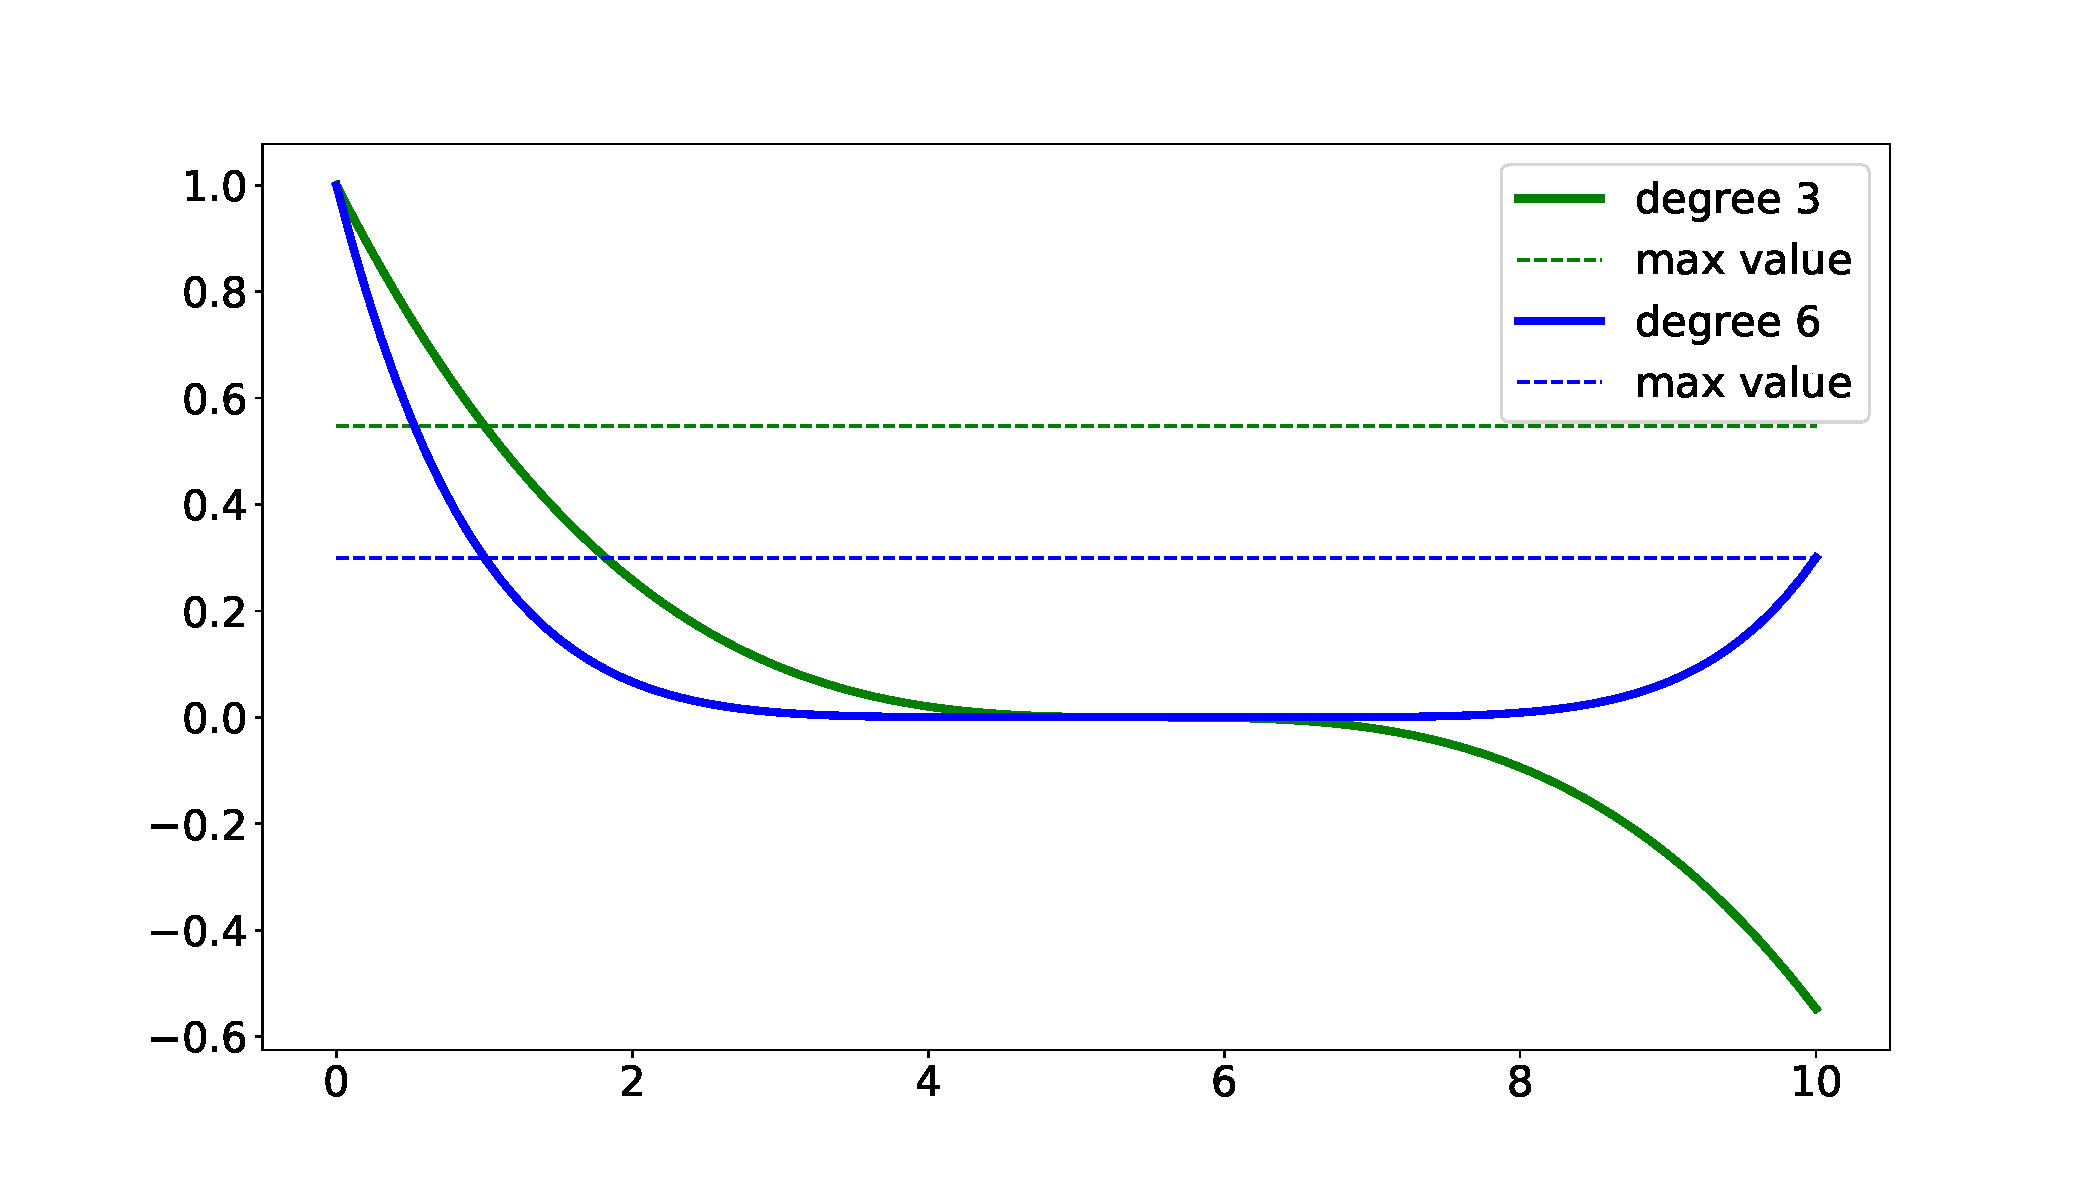
\includegraphics[width=15cm]{figures/lecture6-naive_polynome.pdf}
\centering
\caption{Naive Polynomial}
\label{naive_p}
\end{figure}


The resulting polynomial $p_t(x)$ is plotted in figure \ref{naive_p} for degrees $t = 3$ and $t = 6$, with $\alpha = 1$ and $\beta = 10$. Note that doubling the degree from three to six only halves the maximum absolute value the polynomial attains in $[\alpha,\beta]$, explaining why convergence is so slow.


\subsection{Chebyshev polynomials}
% TODO for Andy: fill in the below, on Chebyshev polynomials.

Fortunately, we can do better than this by speeding up gradient descent using Chebyshev polynomials. The Chebyshev polynomials are a sequence of orthogonal polynomials which are related to de Moivre's formula and which can be defined recursively. We will use Chebyshev polynomials of the first kind which are donated $T_n$.

The Chebyshev polynomials of the first kind are defined by the recurrence relation:
\begin{align*}
T_0(a) &= 1,\quad T_1(a) = a \\
T_k(a) &= 2a T_{k-1}(a) - T_{k-2}(a),\ \text{for }k \geq 2.
\end{align*}
And figure \ref{chebychev_poly} is the plot of the Chebyshev polynomials for $i=0, 1, 2, 3, 4$. 

\begin{figure}[ht]
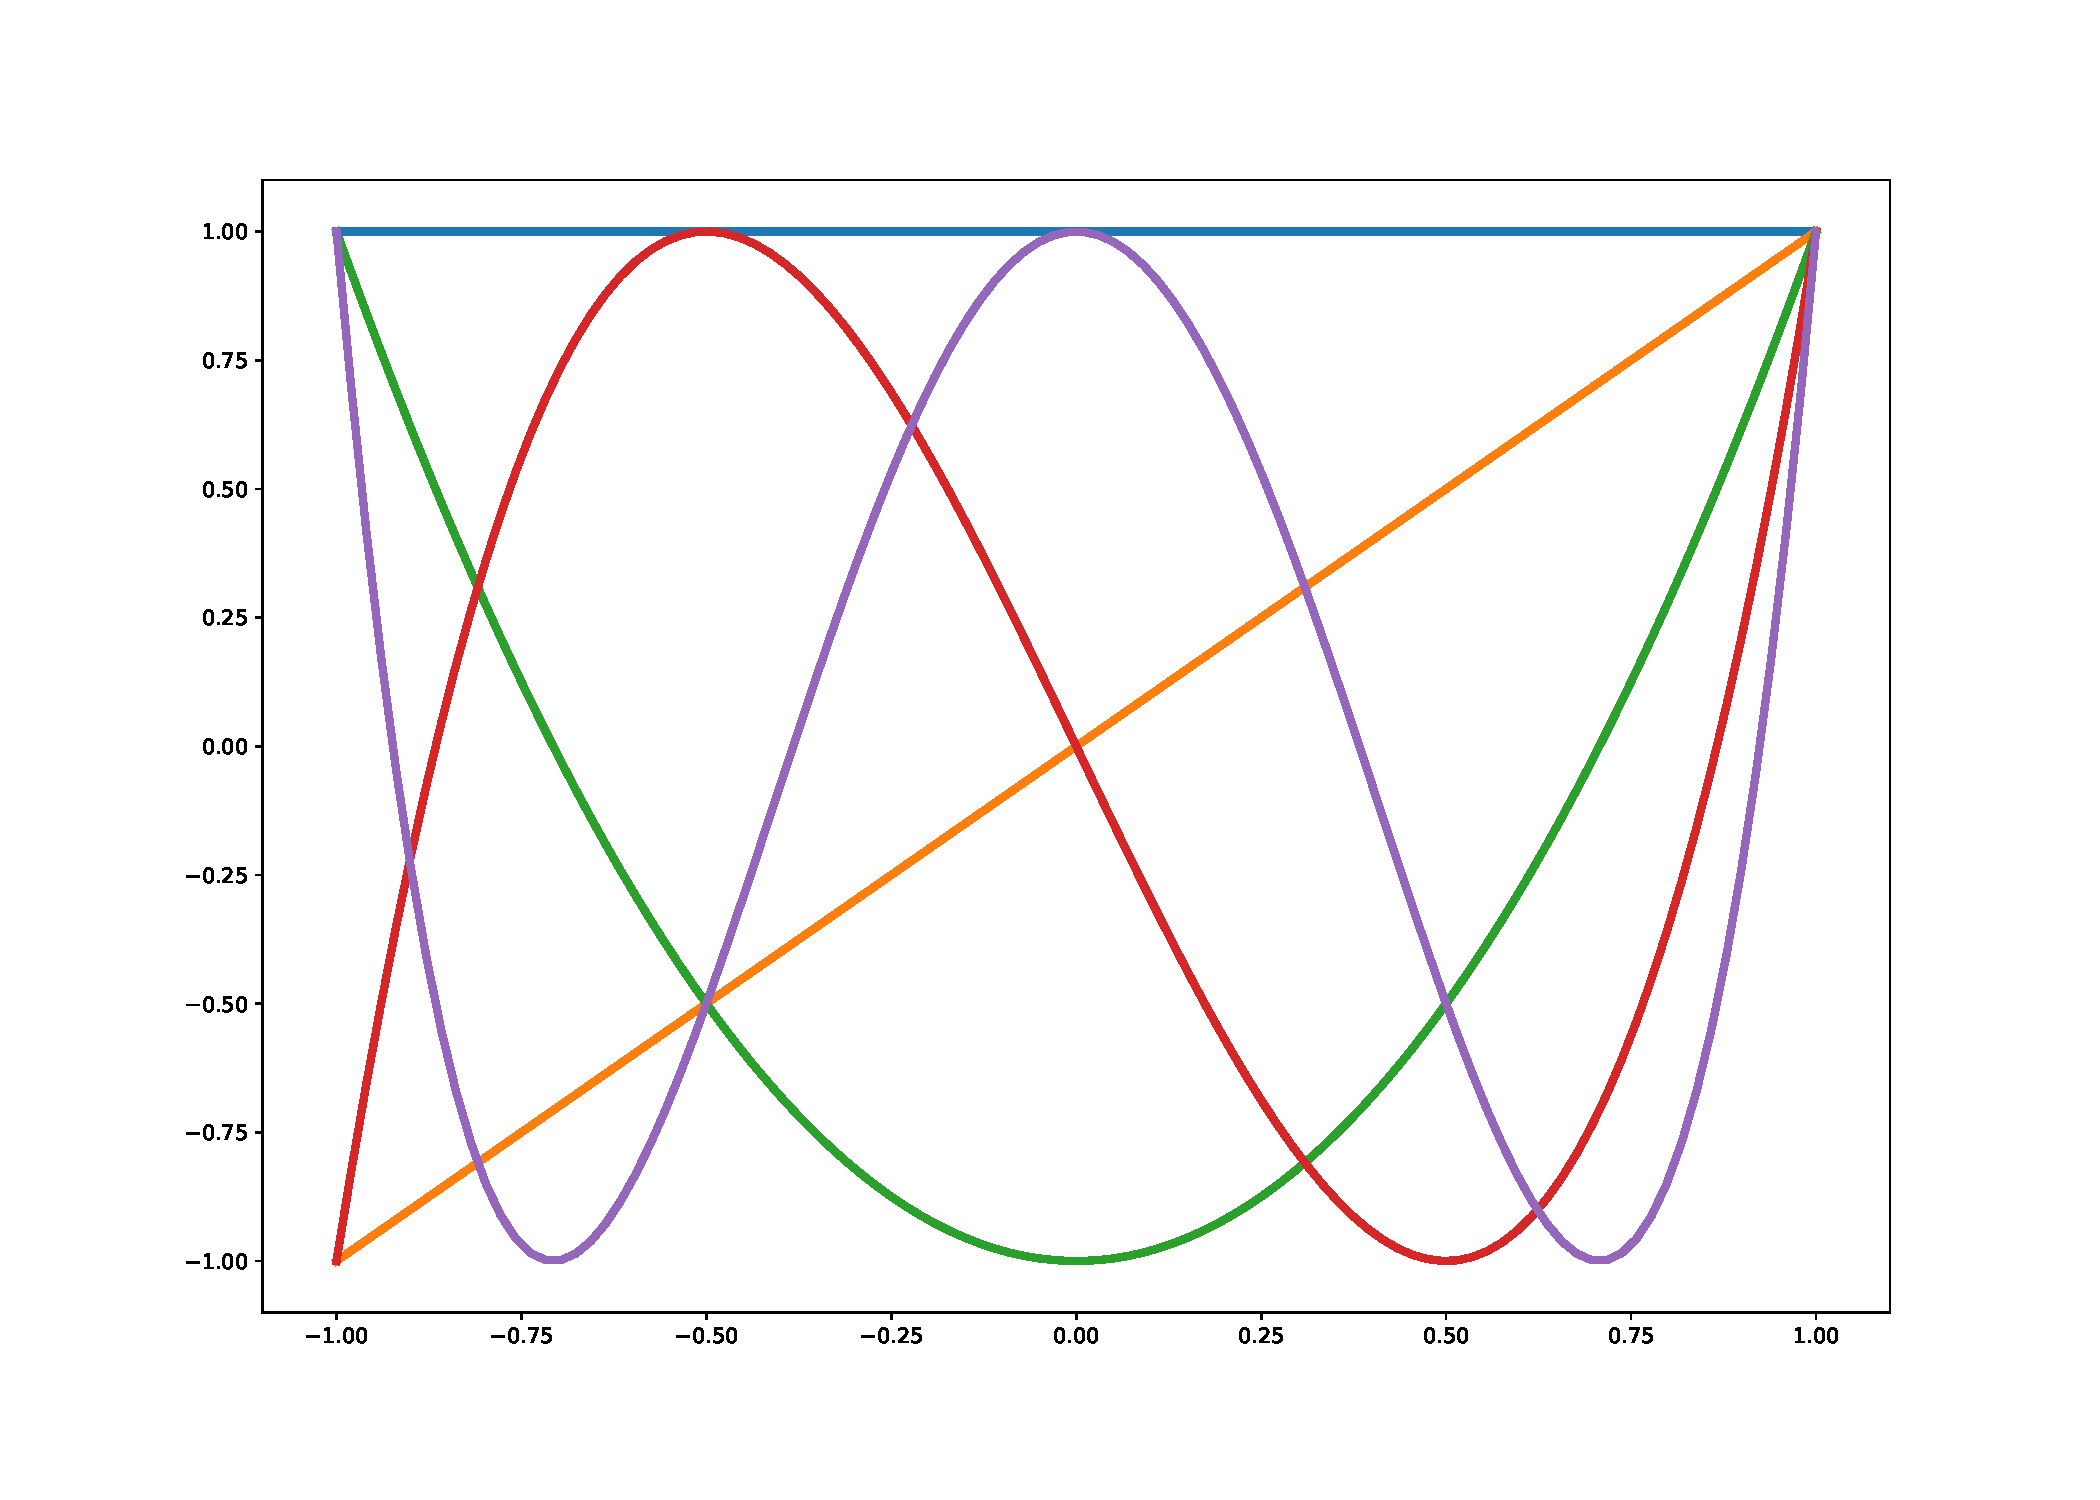
\includegraphics[width=15cm]{figures/lecture6-cheb_polynome.pdf}
\centering
\caption{Chebychev polynomials}
\label{chebychev_poly}
\end{figure}

Why Chebyshev polynomials? Suitably rescaled, they minimize the absolute value in a desired interval $[\alpha, \beta]$ while satisfying the normalization constraint of having value $1$ at the origin.

Recall that the eigenvalues of the matrix we consider are in the interval $[\alpha, \beta]$. We need to rescale the Chebyshev polynomials so that they're supported on this interval and still attain value $1$ at the origin. This is accomplished by the polynomial

\begin{equation*}
P_k(a) = \frac{T_k\left(\frac{\alpha + \beta - 2a}{\beta - \alpha}\right)}{T_k\left(\frac{\alpha + \beta}{\beta - \alpha}\right)}.
\end{equation*}
\begin{figure}[ht]
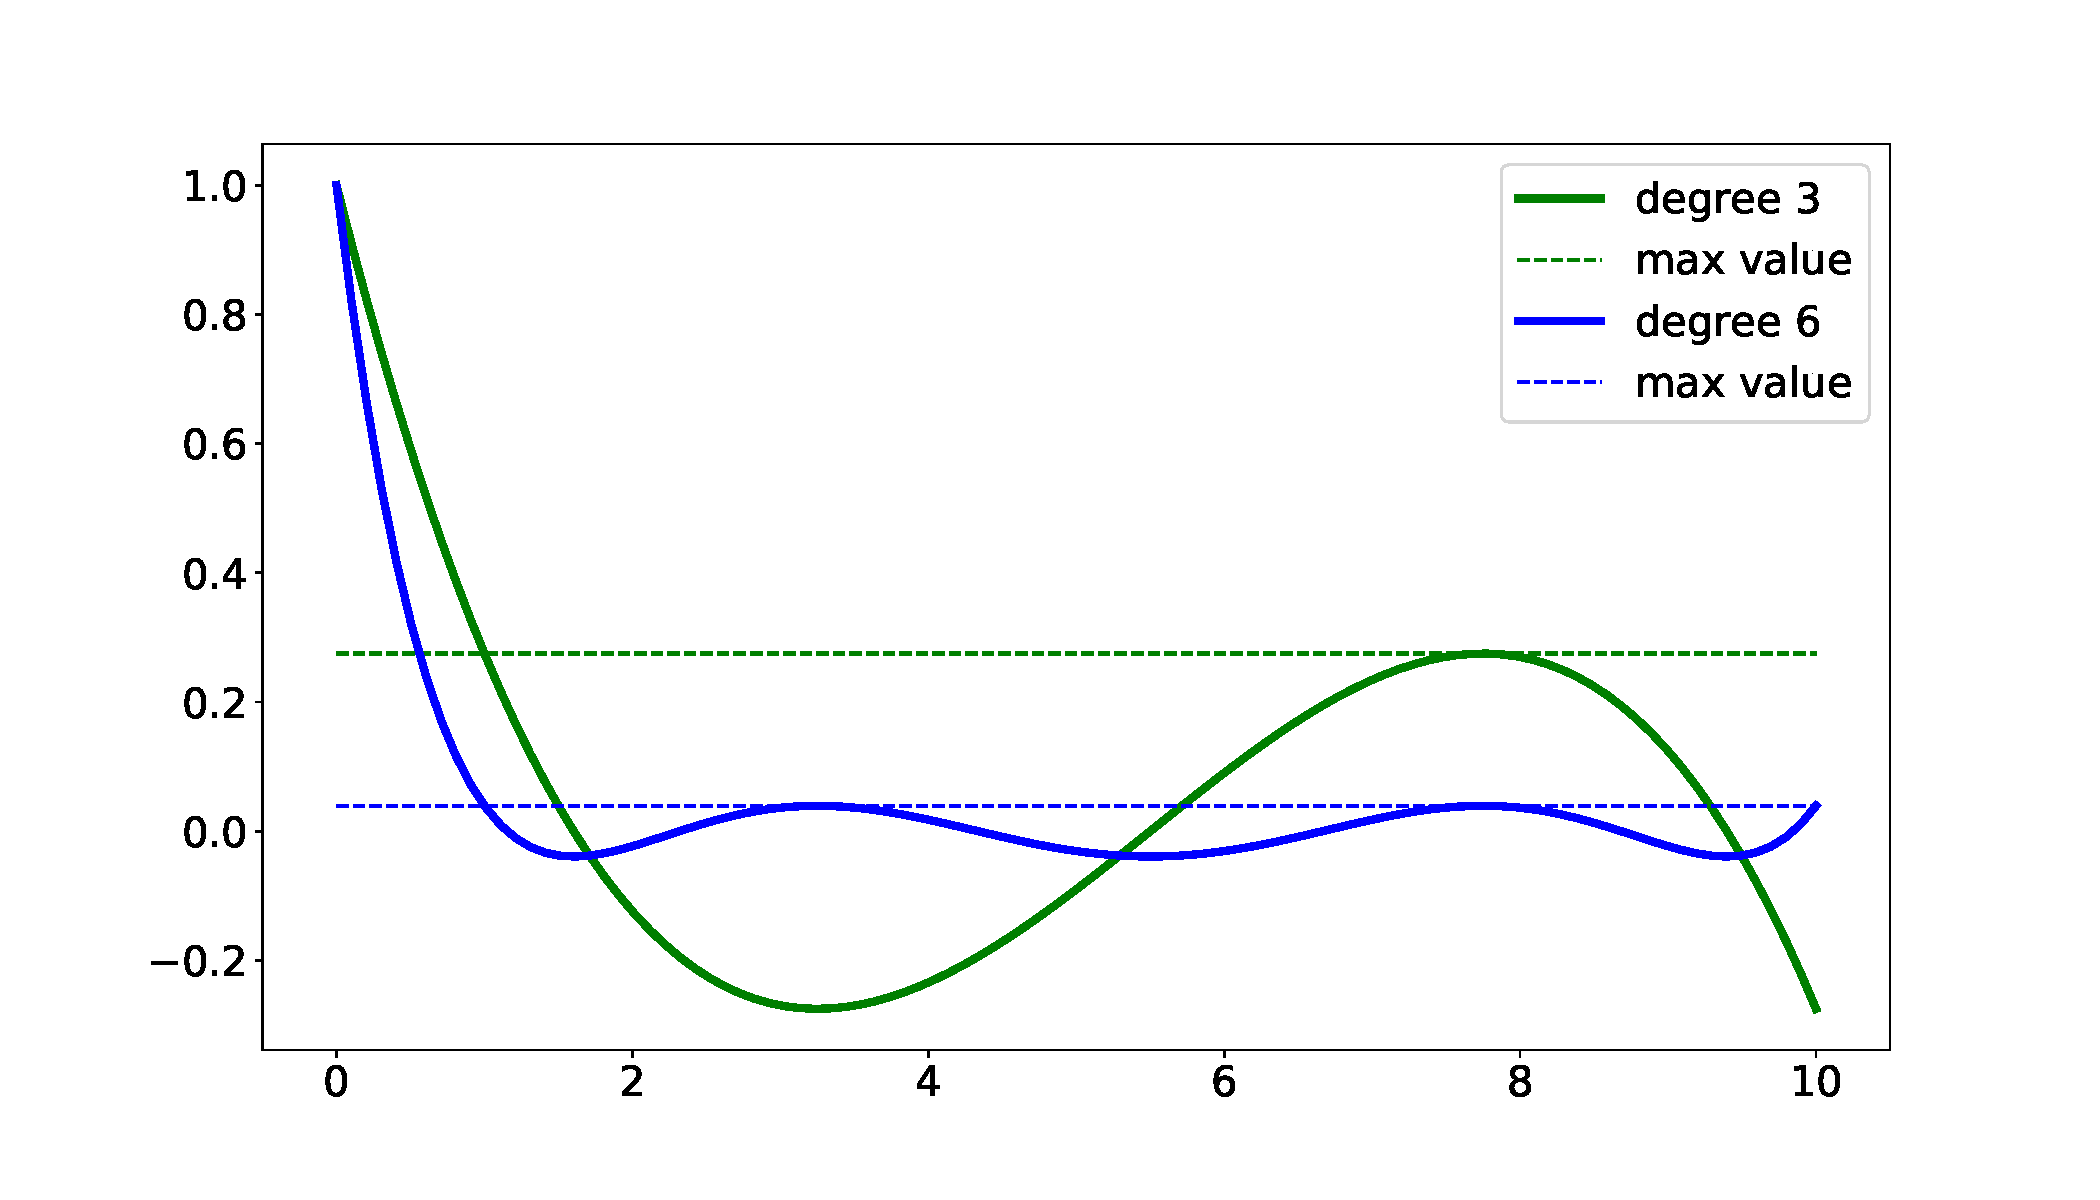
\includegraphics[width=15cm]{figures/lecture6-rescaled_cheb.pdf}
\centering
\caption{Rescaled Chebyshev}
\label{rescales_chebyshev}
\end{figure}

\begin{figure}[ht]
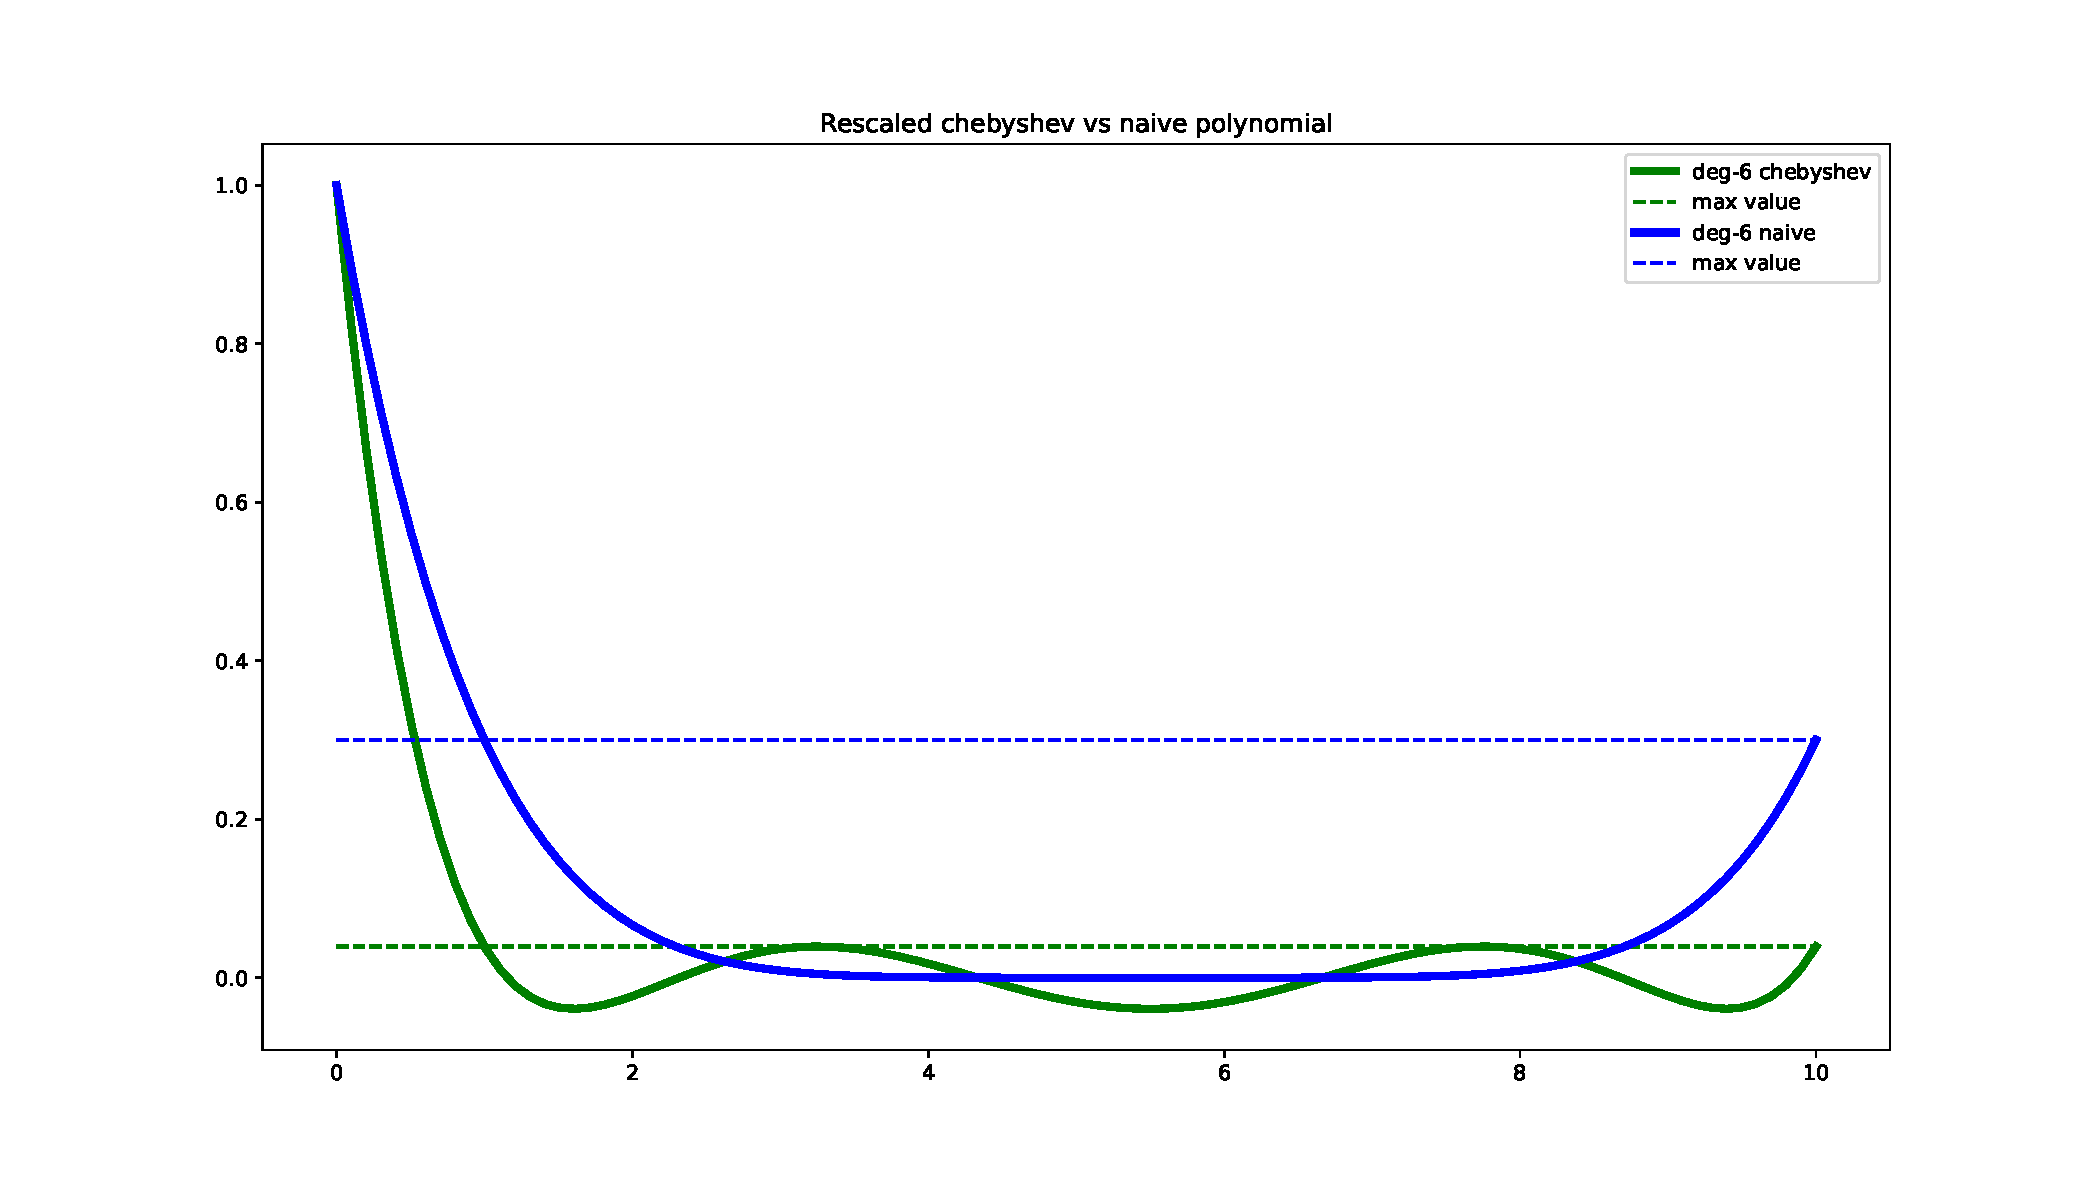
\includegraphics[width=15cm]{figures/lecture6-rescaled_cheb_vs_naive.pdf}
\centering
\caption{Rescaled Chebyshev VS Naive Polynomial}
\label{rescaled_chebyshev_vs_naive_p}
\end{figure}

We see on figure \ref{rescales_chebyshev} that doubling the degree has a much more dramatic effect on the magnitude of the polynomial in the interval $[\alpha, \beta].$

Let's compare on figure \ref{rescaled_chebyshev_vs_naive_p} this beautiful Chebyshev polynomial side by side with the naive polynomial we saw earlier. The Chebyshev polynomial does much better: at around 0.3 for degree 3 (needed degree 6 with naive polynomial), and below 0.1 for degree 6.



\subsubsection{Accelerated gradient descent}

The Chebyshev polynomial leads to an accelerated version of gradient descent. Before we describe the iterative process, let's first see what error bound comes out of the Chebyshev polynomial.

So, just how large is the polynomial in the interval $[\alpha, \beta]$? First, note that the maximum value is attained at $\alpha$. Plugging this into the definition of the rescaled Chebyshev polynomial we get the upper bound for any $a\in[\alpha, \beta],$

\begin{align*}
|P_k(a)| &\leq |P_k(\alpha)| \\
&= \frac{|T_k(1)|}{|T_K\left(\frac{\beta + \alpha}{\beta - \alpha}\right)|} \\
&= {|T_K\left(\frac{\beta + \alpha}{\beta - \alpha}\right)^{-1}|}.
\end{align*}
Recalling the condition number $\kappa=\beta/\alpha,$ we have
\begin{equation*}
\frac{\beta + \alpha}{\beta - \alpha} = \frac{\kappa + 1}{\kappa - 1}.
\end{equation*}
Typically $\kappa$ is large, so this is $1 + \epsilon$, $\epsilon \approx \frac{2}{\kappa}$. Therefore, we have
\begin{eqnarray*}
|P_k(a)| &\leq {|T_k(1 + \epsilon)^{-1}|}.
\end{eqnarray*}

To upper bound $|P_k|$, we need to lower bound $|T_k(1 + \epsilon)|$.

\textbf{Fact}: for $a > 1$, $T_k(a) = \cosh\left(k \cdot \mathrm{arccosh} (a)\right)$ where:
\begin{equation*}
\cosh(a) = \frac{e^a + e^{-a}}{2},\quad \mathrm{arccosh}(a) = \ln\left(x + \sqrt{x^2 - 1}\right).
\end{equation*}

Now, letting $\phi = \mathrm{arccosh}(1 + \epsilon)$:
\begin{equation*}
e^{\phi} = 1 + \epsilon + \sqrt{2\epsilon + \epsilon^2} \geq 1 + \sqrt{\epsilon}.
\end{equation*}
So, we can lower bound $|T_k(1 + \epsilon)|$:
\begin{align*}
|T_k(1 + \epsilon)| &= \cosh\left(k \mathrm{arccosh}(1 + \epsilon)\right) \\
&= \cosh(k\phi) \\
&= \frac{(e^\phi)^k + (e^{-\phi})^k}{2} \\
&\geq \frac{(1 + \sqrt{\epsilon})^k}{2}.
\end{align*}

Then, the reciprocal is what we needed to upper bound the error of our algorithm, so we have:
\begin{equation*}
|P_k(a)| \leq {|T_k(1 + \epsilon)^{-1}|} \leq 2(1 + \sqrt{\epsilon})^{-k}.
\end{equation*}

Thus, this establishes that the Chebyshev polynomial achieves the error bound:
\begin{align*}
\left\Vert X_{t+1} - X^* \right\Vert &\leq 2(1 + \sqrt{\epsilon})^{-t} \left\Vert X_0 -X^*\right\Vert \\
&\approx 2(1 + \sqrt{\frac{2}{\kappa}})^{-t} \left\Vert X_0 -X^*\right\Vert \\
&\leq 2\exp\left(-t \sqrt{\frac{2}{\kappa}}\right) \left\Vert X_0 -X^*\right\Vert.
\end{align*}

This means that for large $\kappa,$ we get quadratic savings in the degree we need before the error drops off exponentially. Figure \ref{convergence} shows the different rates of convergence, we clearly see that the 

\begin{figure}[ht]
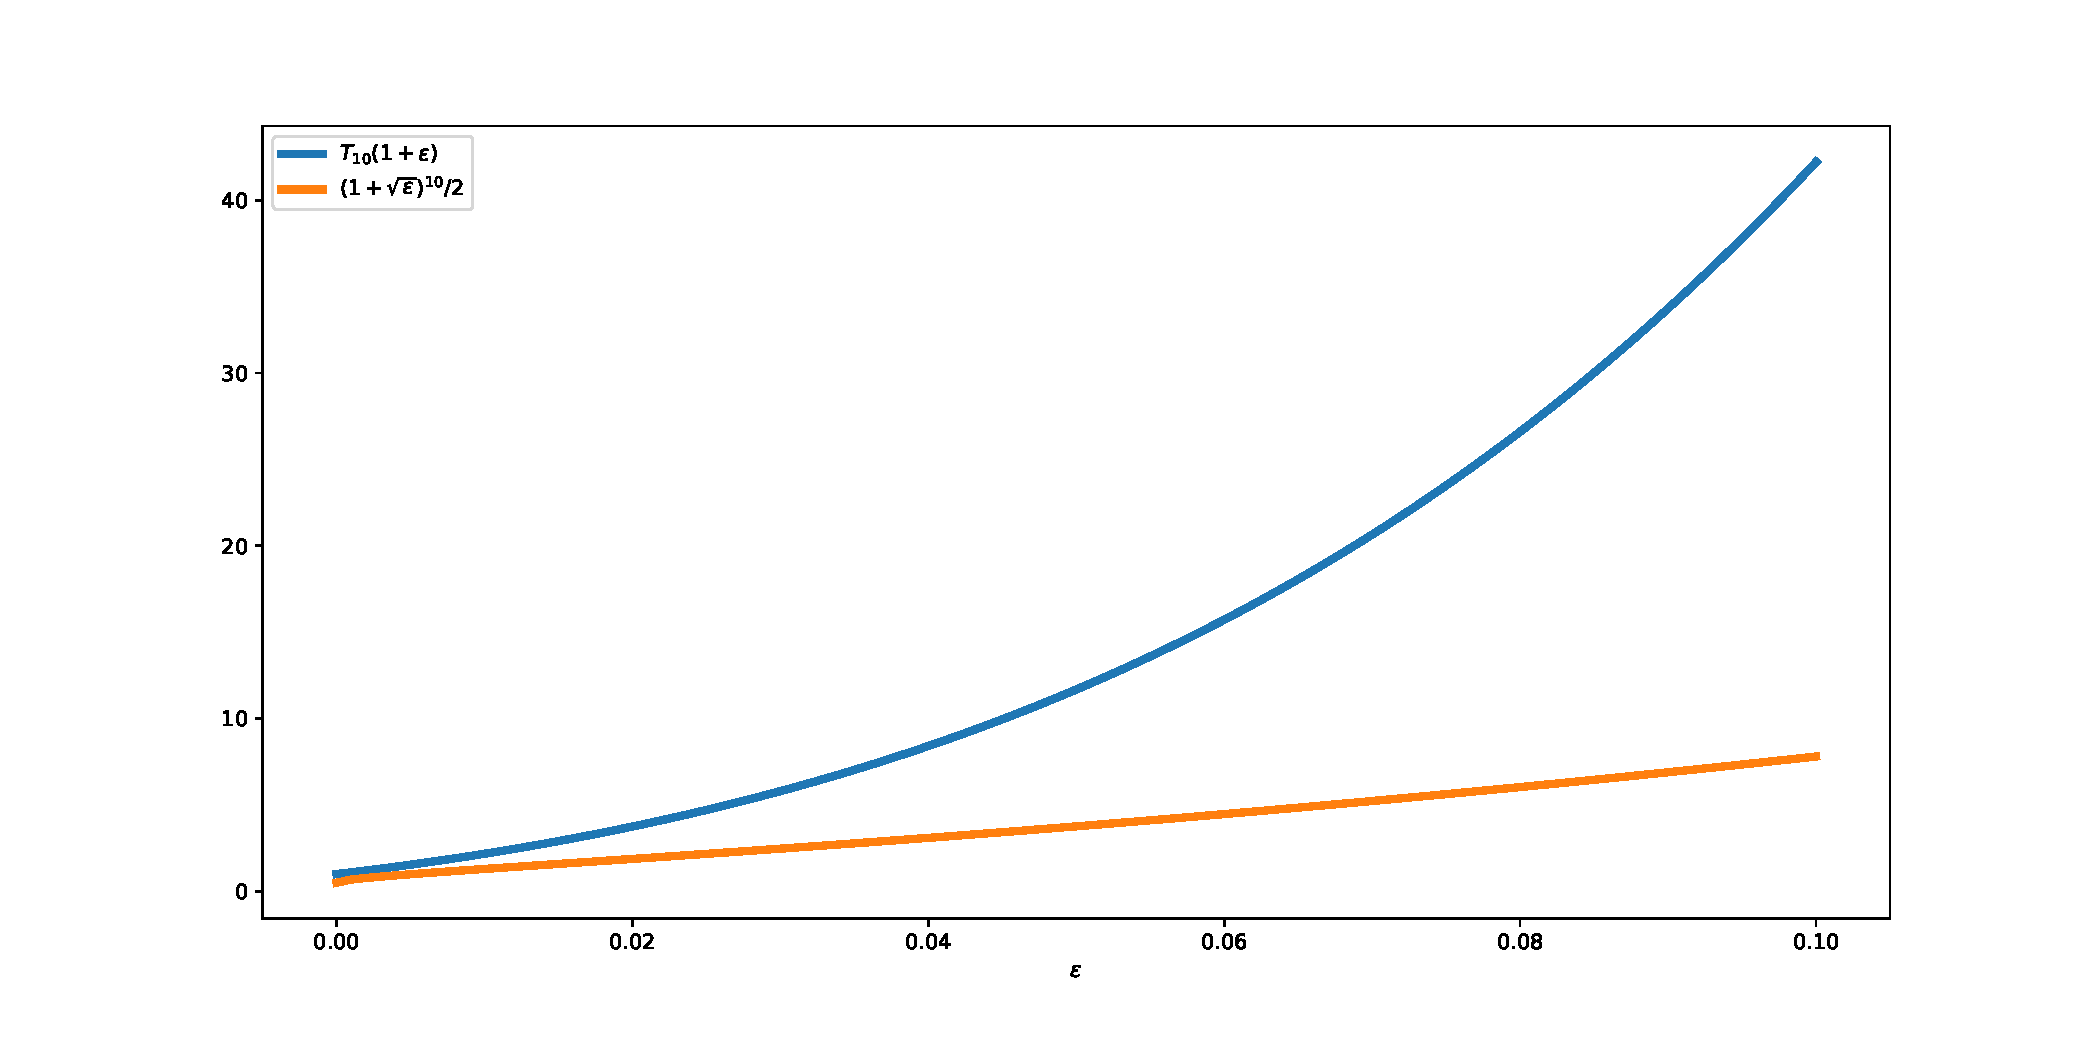
\includegraphics[width=15cm]{figures/lecture6-conv.pdf}
\centering
\caption{Convergence for naive polynomial and Chebyshev}
\label{convergence}
\end{figure}

\subsubsection{The Chebyshev recurrence relation}
Due to the recursive definition of the Chebyshev polynomial, we directly get an iterative algorithm out of it. Transferring the recursive definition to our rescaled Chebyshev polynomial, we have:
\begin{equation*}
P_{K+1}(a) = (\eta_k a + \gamma_k)P_k(a) + \mu_k P_{k-1}(a).
\end{equation*}

where we can work out the coefficients $\eta_k,\gamma_k,\mu_k$ from the recurrence definition. Since $P_k(0)=1,$ we must have $\gamma_k+\mu_k=1.$ This leads to a simple update rule for our iterates:

\begin{eqnarray*}
X_{k+1} &= (\eta_k A + \gamma_k)X_k + (1 - \gamma_K)X_{k-1} - \eta_k b \\
&= (\eta_K A + (1 - \mu_k))X_k + \mu_k X_{k-1} - \eta_k b \\
&= X_k - \eta_k(AX_k - b) + \mu_k(X_k - X_{k-1}).
\end{eqnarray*}

We see that the update rule above is actually very similar to plain gradient descent except for the additional term  $\mu_k(x_k - x_{k-1}).$ This term can be interpreted as a \textit{momentum} term, pushing the algorithm in the direction of where it was headed before. In the next lecture, we'll dig deeper into momentum and see how to generalize the result for quadratics to general convex functions.


\section{Lecture 7: Nesterov’s accelerated gradient descent}

Previously, we saw how we can accelerate gradient descent for minimizing
quadratics~$f(x)=x^\trans A x+b^\trans x,$ where $A$ is a positive definite
matrix. In particular, we achieved a quadratic improvement in the dependence
on the condition number of the matrix~$A$ than what standard gradient descent
achieved.

In this lecture, we will see that this phenomenon extends to arbitrary smooth
convex functions by virtue of Nesterov's celebrated \emph{accelerated gradient
method}~\cite{Nesterov83, Nesterov04}. Specifically, we will see that Nesterov's
method achieves a convergence rate of~$\cO \left(\frac{\beta}{t^2}\right)$ for
$\beta$-smooth functions. For functions which are $\alpha$-strongly convex, we
will achieve a rate of $\exp\left( -\Omega\left(\sqrt{\frac{\beta}{\alpha}}
t\right)\right)$. 

The algorithm proceeds iteratively as follows: 
\begin{align*}
x_0 &= y_0 = z_0, \\
x_{k+1} &= \tau z_k + (1 - \tau) y_k \tag{$k\ge 0$}\\
y_k &= x_k - \frac{1}{\beta} \nabla f(x_k) \tag{$k\ge 1$}\\
z_k &= z_{k -1} - \eta\nabla f(x_k)\tag{$k\ge 1$}
\end{align*}
Here, the parameter~$\beta$ is the smoothness constant of the function we're
minimizing. The step size $\eta$ and the parameter~$\tau$ will be chosen below
so as to give us a convergence guarantee.

\subsection{Convergence analysis}

We first show that for a simple setting of the step sizes, the algorithm reduces
its initial error from some value~$d$ to $\frac{d}{2}.$ We will then repeatedly
restart the algorithm to continue reducing the error. This is a slight departure
from Nesterov's method which does not need restrating, albeit requiring a much
more delicate step size schedule that complicates the analysis.

\begin{lemma}
\lemmalabel{lecture7-main}
Suppose $f\colon\R^n\to\R$ is a convex, $\beta$-smooth function that attains its
minimum at a point~$x^*\in\R^n.$
Assume that the initial point satisfies $\|x_0-x^*\|\le R$ and $f(x_0)-f(x^*)\le
d.$ Put $\eta = \frac{R}{\sqrt{d\beta}}$, and 
$\tau$ s.t. $\frac{1-\tau}{\tau} = \eta \beta$.

Then after $T = 4R\sqrt{\frac{\beta}{d}}$ steps, 
we have 
\[
f(\bar{x})- f(x^*) \leq \frac{d}{2},
\]
where $\bar{x} = \frac{1}{T} \sum_{k=0}^{T-1} x_k$.
\end{lemma}

\begin{proof}
In Lecture~2, we showed the following properties for smooth and convex
functions:
\begin{equation}
\label{Nesterov-pf_smoothness_and_convexity}
f(y_k) - f(x_k) \leq -\frac{1}{2 \beta} \|\nabla f(x_k) \|^2
\end{equation}
By the ``Fundamental Theorem of Optimization" (see Lecture 2), we have
for all $u\in\R^n:$
\begin{align}
\label{lecture7-nonsmooth}
\eta\langle \nabla f(x_{k+1}), z_k - u \rangle 
&= \frac{\eta^2}2\|\nabla f(x_{k+1})\|^2 
+ \frac12\|z_k - u \|^2 - \frac12\|z_{k+1} - u \|^2\,.
\end{align}
Substituting the first equation yields
\begin{equation}
\eta \langle \nabla f(x_{k+1}, z_k - u \rangle \leq \eta^2 \beta (f(x_{k+1}) -
f(y_{k+1})) + \frac12\|z_k - u\|^2 - \frac12\|z_{k+1} - u \|^2 \label{Nesterov-pf_eq3}
\end{equation}
\medskip
Working towards a term that we can turn into a telescoping sum, we compute the
following difference:
\begin{align}
&\eta \langle \nabla f(x_{k+1}), x_{k+1} - u\rangle - \eta \langle \nabla f(x_{k+1}), z_k - u\rangle \nonumber\\
&= \eta \langle\nabla f(x_{k+1}), x_{k+1} - z_k\rangle \nonumber\\
&= \frac{1-\tau}{\tau}  \eta \langle\nabla f(x_{k+1}), y_k - x_{k+1}\rangle \nonumber\\
&\leq \frac{1-\tau}{\tau} \eta (f(y_k) - f(x_{k+1})) \quad\text{ (by convexity)}. \label{Nesterov-pf_eq4}
\end{align}
\medskip
Combining  \eqref{Nesterov-pf_eq3} and \eqref{Nesterov-pf_eq4}, and setting
$\frac{1-\tau}{\tau} = \eta \beta$ yield for all $u\in\R^n:$
\begin{equation*}
\eta\langle\nabla f(x_{k+1}), x_{k+1} - u\rangle \leq \eta^2 \beta
(f(y_k) - f(y_{k+1})) + \frac12\|z_k - u\|^2 - \frac12\|z_{k+1} - u\|^2.
\end{equation*}
Proceeding as in our basic gradient descent analysis, we apply this inequality
for $u=x^*,$ sum it up from $k=0$ to $T$ and exploit the telescoping effect:
\begin{align*}
\eta T (f(\bar{x}) - f(x^*)) 
&\leq \sum_{k=0}^T \eta \langle\nabla f(x_{k+1}), x_{k+1} - x^*\rangle\\
&\leq \eta^2 \beta d + R^2,
\end{align*}
which can be rewritten as
\begin{align*}
f(\bar{x}) - f(x^*) 
&\leq \frac{\eta\beta d}{T} + \frac{R^2}{\eta T} \\
&\leq \frac{2\sqrt{\beta d}}{T} R \tag{since $\eta=R/\sqrt{\beta d}$} \\
&\leq \frac{d}{2} \tag{since $T\ge 4R\sqrt{\beta/D}.$}
\end{align*}
\end{proof}

This lemma appears in work by Allen-Zhu and Orecchia~\cite{allen2014linear}, who
interpret Nesterov's method as a coupling of two ways of analyzing gradient
descent. One is the the inequality
in~\eqref{Nesterov-pf_smoothness_and_convexity} that is commonly used in the
analysis of gradient descent for smooth functions. The other is
Equation~\ref{lecture7-nonsmooth} commonly used in the convergence analysis for
non-smooth functions. Both were shown in our Lecture 2.

\begin{theorem}
\theoremlabel{lecture7-smooth}
Under the assumptions of \lemmaref{lecture7-main}, by restarting the algorithm
repeatedly, we can find a point $x$ such that
\[
f(x)-f(x^*)\le\epsilon
\]
with at most $O(R\sqrt{\beta/\epsilon})$ gradient updates.
\end{theorem}
\begin{proof}
By \lemmaref{lecture7-main}, we can go from error $d$ to $d/2$ with
$CR\sqrt{\beta/d}$ gradient updates for some constant~$C$. 
Initializing each run with the output of
the previous run, we can there for successively reduce the error from an initial
value~$d$ to $d/2$ to $d/4$ and so on until we reach error~$\epsilon$ after
$O(\log(d/\epsilon))$ runs of the algorithm. The total number of gradient steps
we make is
\[
CR\sqrt{\beta/d} 
+CR\sqrt{2\beta/d}
+\dots+CR\sqrt{\beta/\epsilon}
= O\left(R\sqrt{\beta/\epsilon}\right)\,.
\]
Note that the last run of the algorithm dominates the total number of steps up to a
constant factor.
\end{proof}

\subsection{Strongly convex case}

We can prove a variant of \lemmaref{lecture7-main} that applies when the
function is also $\alpha$-strongly convex, ultimately leading to a linear
convergence rate. The idea is just a general trick to convert a convergence rate
for a smooth function to a convergence rate in domain using the definition of
strong convexity.

\begin{lemma}
Under the assumption of \lemmaref{lecture7-main} and the additional assumption
that the function~$f$ is $\alpha$-strongly convex, we 
can find a point~$x$ with $T = O\left(\sqrt{\frac{\beta}{\alpha}}\right)$
gradient updates such that
\[
\|\bar x - x^*\|^2 \leq \frac12\|x_0-x^*\|^2\,.
\]
\end{lemma}
\begin{proof}
Noting that $\|x_0-x^*\|^2\le R^2,$ we can apply \theoremref{lecture7-smooth} with
error parameter $\epsilon = \frac{\alpha}4 \|x_0-x^*\|^2$ to find a point~$x$ such that
\[
f(x)-f(x^*)\le \frac\alpha4\|x_0-x^*\|^2\,,
\]
while only making $O\left(\sqrt{\beta/\alpha}\right)$ many steps.
From the definition of strong convexity it follows that
\[
\frac\alpha2 \|x-x^*\|^2 \le f(x)-f(x^*)\,.
\]
Combining the two inequalities gives the statement we needed to show.
\end{proof}

We see from the lemma that for strongly convex function we actually reduce the
distance to the optimum in domain by a constant factor at each step. We can
therefore repeatedly apply the lemma to get a linear convergence rate.

Table \ref{tab:nesterov} compares the bounds on error $\epsilon(t)$ as a
function of the total number of steps when applying Nesterov's method and
ordinary gradient descent method to different functions. 

\begin{table}[h]
  \begin{center}
    \begin{tabular}{ | l | c | c |}
      \hline
        & Nesterov's Method 
        & Ordinary GD Method \\ \hline
      $\beta$-smooth, convex 
      & \begin{tabular}{c}
        $O\left(\beta/t^2\right)$
        \end{tabular}
      & \begin{tabular}{c}
        $O\left(\beta/t\right)$
        \end{tabular} \\ \hline
      $\beta$-smooth, $\alpha$-strongly convex 
      & \begin{tabular}{c}
        $\exp\left(-\Omega(t\sqrt{\alpha/\beta})\right)$
        \end{tabular} 
      & \begin{tabular}{c}
        $\exp\left(-\Omega(t\alpha/\beta)\right)$
        \end{tabular} \\ \hline
    \end{tabular}
  \end{center}
  \caption{Bounds on error $\epsilon$ as a function of number of iterations $t$ for different methods.}
  \label{tab:nesterov}
\end{table}



\section{Lecture 8: Conjugate gradients and Krylov subspaces}
\sectionlabel{TBD}

In this lecture, we'll develop a unified view of solving linear equations~$Ax=b$
and eigenvalue problems~$Ax=\lambda x.$ In particular, we will justify the
following picture.
%
\begin{center}
\begin{tabular}{ | c |c| c | } 
\hline
 & $Ax=b$ & $Ax=\lambda x$ \\ 
\hline
Basic & Gradient descent & Power method \\ 
\hline
Accelerated & Chebyshev iteration & Chebyshev iteration \\
\hline
Accelerated and step size free & Conjugate gradient & Lanczos \\
\hline
\end{tabular}
\end{center}

What we saw last time was the basic gradient descent method and Chebyshev
iteration for solving quadratics. Chebyshev iteration requires step sizes to be
carefully chosen. In this section, we will see how we can get a ``step-size
free'' accelerated method, known as \emph{conjugate gradient}.

What ties this all together is the notion of a Krylov subspace and its
corresponding connection to low-degree polynomials.

Our exposition follows the excellent Chapter VI
in~Trefethen-Bau~\cite{trefethen97}.

\subsection{Krylov subspaces}
%
The methods we discuss all have the property that they generate a sequence of
points iteratively that is contained in a subspace called the \emph{Kyrlov
subspace}.
%
\begin{definition}[Krylov subspace]
For a matrix $A \in \R^{n x n}$ and a vector $b \in \R^n$, 
the \emph{Krylov sequence} of order $t$ is $b, Ab, A^2b, ...., A^tb$. 
We define the \emph{Krylov subspace} as
\[
K_t(A,b)=\mathrm{span}(\{b, Ab, A^2b, \ldots, A^t\}) \subseteq \R^n\,.
\]
\end{definition}

Krylov subspace naturally connect to polynomial approximation problems.
To see this, recall that a degree~$t$ matrix polynomial is an expression of the form
$p(A)=\sum_{i=1}^t \alpha_i A^i.$ 

\begin{fact}[Polynomial connection]
The Krylov subspace satisfies
\[
K_t(A,b) = \left\{ p(A)b : \text{deg}(p) \leq t \right\}\,.
\]
\end{fact}
\begin{proof}
Note that
\begin{align*}
v \in K_t(A,b) &\Longleftrightarrow \exists \alpha_i: \ v= \alpha_0 b + \alpha_1 Ab + \cdots \alpha_t A^tb
\end{align*}
\end{proof}


From here on, suppose we have a symmetric matrix $A \in \R^{n \times n}$ that
has orthonormal eigenvectors $u_1 \ldots u_n$ and ordered eigenvalues $\lambda_1
\geq \lambda_2 \ldots \geq \lambda_n$. Recall, this means
\begin{align*}
    \langle u_i,u_j\rangle &= 0,\quad\text{for } i \neq j\\
    \langle u_i, u_i\rangle &= 1 
\end{align*}
Using that $A=\sum_i \lambda_i u_i u_i^\trans,$ it follows
\[
p(A)u_i = p(\lambda_i)u_i\,.
\]
%
Now suppose we write $b$ in the eigenbasis of $A$ as 
\[
b=\alpha_1 u_1 + ... + \alpha_n u_n
\] 
with $\alpha_i = \langle u_i,b\rangle$. It follows that
\begin{align*}
p(A)b &= \alpha_1 p(\lambda_1)u_1 + \alpha_2 p(\lambda_2) u_2 + \ldots +
\alpha_n p(\lambda_n) u_n\,.
\end{align*}
 
\subsection{Finding eigenvectors}
Given these ideas, one natural approach to finding eigenvectors is to find a
polynomial~$p$ such that
\[
p(A)b \approx \alpha_1 u_1\,.
\]
Ideally, we would have $p(\lambda_1) = 1$ and $ p(\lambda_i) = 0$ for $i > 1$,
but this is in general impossible unless we maket he degree of our polynomial as
high as the number of distinct eigenvalues of~$A.$ Keep in mind that the degree
ultimately determines the number of steps that our iterative algorithm makes.
We'd therefore like to keep it as small as possible.

That's why we'll settle for an approximate solution that has $p(\lambda_1) = 1$
and makes $\max_{i > 1} p(\lambda_i)$ as small as possible. This will give us a close
approximation to the top eigenvalue. In practice, we don't know the
value~$\lambda_1$ ahead of time. What we therefore really care about is the
ratio $p(\lambda_1)/p(\lambda_2)$ so that no matter what~$\lambda_1,$ the second
eigenvalue will get mapped to a much smaller value by~$p.$ 

We consider the following simple polynomial~$p(\lambda)=\lambda^t$ that 
satisfies
\begin{align*}
    p(\lambda_2)/p(\lambda_1) &= \left(\frac{\lambda_2}{\lambda_1}\right)^t
\end{align*}
In the case where $\lambda_1=(1+\epsilon)\lambda_2$ we need $t=O(1/\epsilon)$ 
to make the ratio small.

The next lemma turns a small ratio into an approximation result for the
top eigenvector. To state the lemma, we recall that $\tan \angle (a,b)$ is the
tangent of the angle between $a$ and $b.$

\begin{lemma}
$\tan \angle(p(A)b, u_1) \leq \max_{j>1} \frac{|p(\lambda_j)|}{|p(\lambda_1)|}
\tan \angle (b, u_1)$
\end{lemma}

\begin{proof}
We define $\theta = \angle (u_1,b)$. By this, we get
\begin{align*}
    \sin ^2 \theta &=  \sum_{j >1} \alpha_j^2 \\
    \cos ^2 \theta &= |\alpha_1|^2 \\
    \tan^2 \theta &= \sum_{j > 1} \frac{|\alpha_j^2|}{|\alpha_1|^2}
\end{align*}
Now we can write:
\begin{align*}
    \tan^2 \angle (p(A)b, u_1) = \sum_{j>1}
\frac{|p(\lambda_j)\alpha_j|^2}{|p(\lambda_1)\alpha_1|^2} \leq
\underset{j>1}{\text{max}} \frac{|p(\lambda_j)|^2}{|p(\lambda_1)|^2} \sum_{j>1} \frac{\alpha_j |^2}{|\alpha_1| ^2}
\end{align*}
We note that this last sum $ \sum_{j > 1} \frac{\alpha_j |^2}{|\alpha_1| ^2}= \tan \theta$ and we obtain our desired result.
\end{proof}
Applying the lemma to $p(\lambda) = \lambda^t$ and $\lambda_1 =
(1+\epsilon) \lambda_2$, we get  
\[
\tan \angle(p(A)b, u_1) \leq
(1+\epsilon)^{-t} \tan \angle(u_1, b)\,.
\]
If there is a big gap between
$\lambda_1$ and $\lambda_2$ this converges quickly but it can be slow if
$\lambda_1 \approx \lambda_2$. It worth noting that if we choose $b\in\R^n$ to be a
random direction, then
\[
\E\left[\tan\angle(u_1,b)\right]=O\left(\sqrt{n}\right)\,.
\]
Going one step further we can also see that the expression $p(A)b=A^tb$ can of
course be built iteratively by repeatedly multiplying by~$A.$ For reasons of
numerical stability it makes sense to normalize after each matrix-vector
multiplication. This preserved the direction of the iterate and therefore does
not change our convergence analysis. The resulting algorithms is the well known
power method, defined recursively as follows:
%
\begin{align*}
x_0 &= \frac{b}{\|b\|} \\
x_t &= \frac{A x_{t-1}}{\|Ax_{t-1}\|}
\end{align*}
%
This method goes back more than hundred years to a paper by M\"untz in 1913, but
continues to find new applications today.
%
\subsection{Applying Chebyshev polynomials}

As we would expect from the development for quadratics, we can use Chebyshev
polynomials to get a better solution the polynomial approximation problem that
we posed above. The idea is exactly the same with the small difference that we
normalize our Chebyshev polynomial slightly differently.  This time around, we
want to ensure that $p(\lambda_1) = 1$ so that we are picking out the first
eigenvalue with the correct scaling. 

%\begin{tikzpicture}[scale = 0.8]
%  %\begin{axis}[doma
%  in= 2:8,xlabel=$\lambda$,label style={font=\large},tick label style={font=\large}, ylabel style={yshift=-.1cm}, xmin=0, xmax=13, ymin=-1, ymax=1.5, xtick={}, ytick={-1, 0,1},trig format plots=rad,grid=both,grid style={dashed,gray}]
%        \begin{axis}[%
%                width=10cm,
%                height=4cm,
%                scale only axis,
%                xmin=0, xmax=7,
%                xtick={0.5, 1, 1.5,2, 2.5,3, 3.5,4, 4.5, 5, 5.5, 5.75, 6,6.5},
%                xticklabels={$\lambda_n$,,,,,,,,,,,$\lambda_1$},
%                xmajorgrids,
%                ymin=-1, ymax=1.2,
%                ymajorgrids,
%                title={$p(0) = 1$},
%                axis lines*=left,
%                line width=1.0pt,
%                mark size=2.0pt,
%                legend style={at={(1.03,1)},anchor=north west,draw=black,fill=white,align=left}];
%                \addplot[domain = 0.5:5.75, black, very thick,samples=200] {.5*(cos(3*deg(x) ))};
%                \addplot[domain = 0:2] coordinates {(0,1)(0.5,0)};
%                \addplot[domain = 6.17:8.3] coordinates {(5.75,0)(6.45,1)};
%                \addplot[red] coordinates{(0.5,1)(0.5,-1)};
%                \addplot[red] coordinates{(5.75,1)(5.75,-1)};
%              
%               
%\end{axis}
%\end{tikzpicture}
%\begin{tikzpicture}[scale = 0.8]
%        \begin{axis}[%
%                width=10cm,
%                height=4cm,
%                scale only axis,
%                xmin=0, xmax=7,
%                xtick={0.5, 1, 1.5,2, 2.5,3, 3.5,4, 4.5, 5, 5.5, 6,6.5,7},
%                xticklabels={$\lambda_n$,,,,,,,,,,,,$\lambda_1$},
%                xmajorgrids,
%                ymin=-1, ymax=1.2,
%                ymajorgrids,
%                title={$p(\lambda_1) = 1$},
%                axis lines*=left,
%                line width=1.0pt,
%                mark size=2.0pt,
%                legend style={at={(1.03,1)},anchor=north west,draw=black,fill=white,align=left}];
%                \addplot[domain = 0.5:5.75, black, very thick,samples=200] {.5*(cos(3*deg(x) ))};
%                \addplot[domain = 0:2] coordinates {(0,1)(0.5,0)};
%                \addplot[domain = 6.17:8.3] coordinates {(5.75,0)(6.45,1)};
%                \addplot[red] coordinates{(0.5,1)(0.5,-1)};
%                \addplot[red] coordinates{(6.5,1)(6.5,-1)};
%              
%               
%\end{axis}
%\end{tikzpicture}

\begin{lemma}
A suitably rescaled degree $t$ Chebyshev polynomial achieves 
\begin{equation*}
\min_{p(\lambda_1)=1} \max_{\lambda \in [\lambda_2, \lambda_n]} p(\lambda) \leq
\frac{2}{(1+\max\{\sqrt{\epsilon},\epsilon\})^t}
\end{equation*}
where $\epsilon = \frac{\lambda_1}{\lambda_2} - 1$ quantifies the gap between the first
and second eigenvalue.
\end{lemma}

Note that the bound is much better than the previous one when~$\epsilon$ is
small. In the case of quadratics, the relevant ``$\epsilon$-value'' was the inverse
condition number. For eigenvalues, this turns into the gap between the first and
second eigenvalue.

\begin{center}
\begin{tabular}{ | c |c| c | } 
\hline
 & $Ax=b$ & $Ax=\lambda x$ \\ 
\hline
$\epsilon$ & $\frac{1}{\kappa} = \frac{\alpha}{\beta}$ & $\frac{\lambda_1}{\lambda_2} -1$ \\ 
\hline
\end{tabular}
\end{center}

As we saw before, Chebyshev polynomials satisfy a recurrence relation that can
be used to derive an iterative method achieving the bound above. The main
shortcoming of this method is that it needs information about the location of
the first and second eigenvalue. Instead of describing this algorithm, we move
on to an algorithm that works without any such information.

\subsection{Conjugate gradient method}
At this point, we switch back to linear equations~$Ax=b$ for a symmetric
positive definite matrix~$A\in\R^{n\times n}.$ The method we'll see is called
\emph{conjugate gradient} and is an important algorithm for solving linear
equations. Its eigenvalue analog is the Lanczos method. While the ideas behind
these methods are similar, the case of linear equations is a bit more intuitive.
%
\begin{definition}[Conjugate gradient method]
We want to solve $Ax = b,$ with  $A\succ 0$ symmetric. The conjugate gradient
method maintains a sequence of three points:
\begin{align*}
x_0 &= 0 \tag{ ``candidate solution''} \\
r_0 &= b \tag{ ``residual''} \\
p_0 &= r_0 \tag{ ``search direction''}
\end{align*}
For $t \ge 1:$
\begin{align*}
\eta_t &= \frac{\|r_{t-1}\|^2}{\langle p_{t-1}, Ap_{t-1}\rangle} \tag{``step size''} \\
x_t &= x_{t-1} + \eta_t p_{t-1} \\
r_t &= r_{t-1} - \eta_t A p_{t-1} \\
p_t &= r_t + \frac{\|r_t\|^2}{\|r_{t-1}\|^2}p_{t-1}
\end{align*}
\end{definition}

\begin{lemma}
\lemmalabel{lecture8-conjugategradient}
The following three equations must always be true for the conjugate gradient
method algorithm:
\begin{itemize}
\item $\mathrm{span}(\{r_0, ...r_{t-1}\}) = K_t(A,b)$
\item For $j<t$ we have $\langle r_t, r_j\rangle = 0$ and in particular
$r_t \perp K_t(A,b).$
\item The search directions are conjugate $p_i^{\trans} A p_j = 0$ for $i\ne j.$
\end{itemize}
\end{lemma}
\begin{proof}
Proof by induction (see Trefethen and Bau). Show that the conditions are true
initially and stay true when the update rule is applied.  
\end{proof}

\begin{lemma}
Let $\|u\|_A = \sqrt{u^\trans A u}$ and $\langle u,v\rangle_A = u^\trans A v$ and 
$e_t = x^* - x_t$. Then $e_t$ minimizes $\|x^* - x\|_A$ over all vectors $x \in K_{t-1}$.
\end{lemma}

\begin{proof}
We know that $x_t \in K_t$. Let $x \in K_t$ and define $x = x_t - \delta$. 
Then, $e = x^* - x = e_t + \delta.$
We compute the error in the $A$ norm:
\begin{align*}
\|x^* - x\|_A^2 
&= (e_t + \delta)^{\trans} A(e_t + \delta) \\
&= e_t^{\trans}Ae_t + \delta^{\trans}A\delta + 2e_t^{\trans} A \delta\,
\end{align*}
Bby definition~$e_t^{\trans}A = r_t$.
Note that $\delta \in K_t.$ 
By \lemmaref{lecture8-conjugategradient}, we have that $r_t \perp K_t(A,b).$
Therefore, $2e_t^{\trans} A \delta = 0$ and hence, 
\begin{align*}
\|e\|_A^2
= \|x^* - x\|_A^2 
= e_t^{\trans}Ae_t + \delta^{\trans}A\delta
\ge \|e_t\|_A\,.
\end{align*}
In the last step we used that $A\succ0.$
\end{proof}

What the lemma shows, in essence, is that conjugate gradient solves the
polynomial approximation problem:
\[
\min_{p\colon\deg(p)\le t, p(0)=1} \|p(A)e_0\|_A\,.
\]
Moreover, it's not hard to show that
\[
\min_{p\colon\deg(p)\le t, p(0)=1} 
\frac{\|p(A)e_0\|_A}{\|e_0\|_A}
\le 
\min_{p\colon\deg(p)\le t, p(0)=1} 
\max_{\lambda\in\Lambda(A)}\left| p(\lambda)\right|\,.
\]
In other words, the error achieved by conjugate gradient is no worse that the
error of the polynomial approximation on the RHS, which was solved by the
Chebyshev approximation. From here it follows that conjugate gradient must
converge at least as fast in $\|\cdot\|_A$-norm than Chebyshev iteration.


\section{Lecture 9: Lower bounds and trade-offs with robustness}

In the first part of this lecture, we study whether the convergence rates
derived in previous lectures are tight. For several classes of optimzation
problems (smooth, strongly convex, etc), we prove the
answer is indeed yes. The highlight of this analysis is to show the $O(1/t^2)$
rate achieved by Nesterov's accelerated gradient method is optimal (in a weak
technical sense) for smooth, convex functions. 

In the second part of this lecture, we go beyond studying convergence rates and
look towards other ways of comparing algorithms. We show the improved rates of
accelerated gradient methods come at a cost in robustness to noise. In
particular, if we restrict ourselves to only using approximate gradients, the
standard gradient method suffers basically no slowdown, whereas the accelerated
gradient method accumulates errors linearly in the number of iterations.

\subsection{Lower bounds}
Before launching into a discussion of lower bounds, it's helpful to first recap
the upper bounds obtained thus far. For a convex function $f$,
Table~\eqref{table:upper-bounds} summarizes the assumptions and rates proved in
the first several lectures. 
~
\begin{table}[]
\centering
\caption{Upper Bounds from Lectures 2-8}
\label{table:upper-bounds}
\begin{tabular}{|l|l|l|}
\hline
$f$                        & Algorithm                    & Rate                                            \\ \hline
Convex, Lipschitz          & Gradient Descent             & $RL / \sqrt{t}$                               \\ \hline
Strongly Convex, Lipschitz & Gradient Descent             & $L^2 / (\alpha t)$                \\ \hline
Convex, Smooth             & Accelerated Gradient Descent & $\beta R^2 / t^2$ \\ \hline
\end{tabular}
\end{table}  

Each of the rates in Table~\eqref{table:upper-bounds} is obtained using some variant of the
gradient method. These algorithms can be thought of as a procedure that
maps a history of points and subgradients $(x_1, g_1, \dots, x_t, g_t)$ to a 
new point $x_{t+1}$. To prove lower bounds, we restrict the class of algorithms 
to similar procedures. Formally, define a black-box procedure as follows.

\begin{definition}[Black-Box Procedure]
A \textit{black-box procedure} generates a sequence of points $\set{x_t}$
such that
\begin{align*}
    x_{t+1} \in x_0 + \Span\set{g_1, \dots, g_t},
\end{align*}
and $g_s \in \partial f (x_s)$.
\end{definition}
Throughout, we will further assume $x_0 = 0$. As expected, gradient descent is a
black-box procedure. Indeed, unrolling the iterates, $x_{t+1}$ is given by
\begin{align*}
    x_{t+1} 
    &= x_t - \eta \grad f(x_t) \\
    &= x_{t-1} - \eta \grad f(x_{t-2}) - \eta \grad f(x_{t-1}) \\
    &= x_0 - \sum_{i=0}^t \eta \grad f (x_i).
\end{align*}

We now turn to proving lower bounds on the convergence rate for any 
black-box procedure.
Our first theorem concerns the constrained, non-smooth case.
The theorem is originally from \cite{nesterov83}, but the presentation will
follow \cite{nesterov04}.
~
\begin{theorem}[Constrainted, Non-Smooth $f$]\label{theorem:lb-non-smooth}
Let $t \leq n$, $L, R  > 0$. There exists a convex $L$-Lipschitz function $f$
such that any black-box procedure satisfies
\begin{align}
    \min_{1 \leq s \leq t} f(x_s) - \min_{x \in B_2(R)} f(x)
    \geq \frac{RL}{2(1+\sqrt{t})}.
\end{align}
Furthermore, there is an $\alpha$-strongly convex, $L$-Lipschitz function $f$
such that
\begin{align}
    \min_{1 \leq s \leq t} f(x_s) - \min_{x \in B_2(\frac{L}{2\alpha})} f(x)
    \geq \frac{L^2}{8\alpha t}.
\end{align}
\end{theorem}
The proof strategy is to exhibit a convex function $f$ so that, for any black-box procedure,
$\Span\set{g_1, g_2, \dots, g_i} \subset \Span\set{e_1, \dots, e_i}$, where
$e_i$ is the $i$-th standard basis vector. After $t$ steps for $t < n$, at least
$n-t$ coordinates are exactly 0, and the theorem follows from lower bounding the
error for each coordinate that is identically zero. 

\begin{proof}
Consider the function
\begin{align*}
    f(x) = \gamma \max_{1 \leq i \leq t} x[i] + \frac{\alpha}{2} \|x\|^2,
\end{align*}
for some $\gamma, \alpha \in \R$. In the strongly convex case, $\gamma$ is
a free parameter, and in the Lipschitz case both $\alpha$ and $\gamma$ are
free parameters. By the subdifferential calculus,
\begin{align*}
    \partial f(x) 
        = \alpha x + \gamma \conv\set{e_i \colon i \in \argmax_{1 \leq j \leq t} x(j)}.
\end{align*}
The function $f$ is evidently $\alpha$-strongly convex. Furthermore, if $\|x\| \leq R$
and $g \in \partial f(x)$, then $\|g\| \leq \alpha R + \gamma$, so $f$ is
$(\alpha R + \gamma)$-Lipschitz on $B_2(R)$.

Suppose the gradient oracle returns $g_i = \alpha x + \gamma e_i$, where
$i$ is the first coordinate such that $x[i] = \max_{1 \leq j \leq t} x[j]$. 
An inductive argument then shows
\begin{align*}
    x_s \in \Span\set{e_1, \dots, e_{s-1}}
\end{align*}
Consequently, for $s \leq t$, $f(x_s) \geq 0$. However, consider $y\in \R^n$
such that
\begin{align*}
    y[i] = 
    \begin{cases}
        -\frac{\gamma}{\alpha t} &\text{if } 1 \leq i \leq t\\
        0 &\text{otherwise}.
    \end{cases}
\end{align*}
Since $0 \in \partial f(y)$, $y$ is an minimizer of $f$ with objective value
\begin{align*}
    f(y)
    = \frac{-\gamma^2}{\alpha t} + \frac{\alpha}{2}\frac{\gamma^2}{\alpha^2 t}
    = -\frac{\gamma^2}{2\alpha t},
\end{align*}
and hence $f(x_s) - f(y) \geq \frac{\gamma^2}{2 \alpha t}$.
We conclude the proof by appropriately choosing $\alpha$ and $\gamma$. 
In the convex, Lipschitz case, set 
\begin{align*}
    \alpha = \frac{L}{R} \frac{1}{1 + \sqrt{t}}
    \quad
    \text{and}
    \quad
    \gamma = L \frac{\sqrt{t}}{1 + \sqrt{t}}.
\end{align*}
Then, $f$ is $L$-Lipschitz, 
\begin{align*}
    \norm{y} 
    = \sqrt{t \Paren{\frac{-\gamma}{\alpha t}}^2}
    = \frac{\gamma}{\alpha \sqrt{t}}
    = R
\end{align*}
and hence
\begin{align*}
    f(x_s) - \min_{x \in B_2(R)} f(x)
    = f(x_s) - f(y)
    \geq \frac{\gamma^2}{2\alpha t}
    = \frac{RL}{2(1+\sqrt{t})}.
\end{align*}
In the strongly-convex case, set $\gamma = \frac{L}{2}$ and take
$R = \frac{L}{2\alpha}$. Then, $f$ is $L$-Lipschitz, 
\begin{align*}
    \norm{y} 
    = \frac{\gamma}{\alpha \sqrt{t}}
    = \frac{L}{2\alpha \sqrt{t}}
    = \frac{R}{\sqrt{t}}
    \leq R,
\end{align*}
and therefore
\begin{align*}
    f(x_s) - \min_{x \in B_2(L/2\alpha)} f(x)
    = f(x_s) - f(y)
    \geq \frac{LR}{4t} 
    = \frac{L^2}{8\alpha t}.
\end{align*}
\end{proof}

Next, we study the smooth, convex case and show the $O(1/t^2)$ rate achieved by
accelerated gradient descent is optimal.

\begin{theorem}[Smooth-$f$]\label{theorem:lb-smooth}
Let $t \leq \frac{n-1}{2}$, $\beta > 0$. There exists a $\beta$-smooth convex
quadratic $f$ such that any black-box method satisfies
\begin{align}
    \min_{1 \leq s \leq t} f(x_s) - f(x^\star)
    \geq \frac{3\beta \norm{x_0 - x^\star}_2^2}{32(t+1)^2}.
\end{align}
\end{theorem}
Similar to the previous theorem, the proof strategy is to exhibit 
a pathological convex function. In this case, we choose what Nesterov calls
``the worst-function in the world'' \cite{nesterov04}.

\begin{proof}
Without loss of generality, let $n = 2t+1$.
Let $L \in \R^{n \times n}$ be the tri-diagonal matrix
\begin{align*}
    L =
    \begin{bmatrix}
        2 & -1 & 0 & 0 & \cdots & 0 \\
        -1 & 2 & -1 & 0 & \cdots & 0 \\
        0 & -1 & 2 & -1  & \cdots & 0 \\
        \vdots & \vdots & \vdots & \vdots & \ddots & \vdots \\
        0 & 0 & 0 & 0 & \cdots -1 & 2  \\
    \end{bmatrix}.
\end{align*}
The matrix $L$ is almost the Laplacian of the cycle
graph (in fact, it's the Laplacian of the chain graph).\footnote{\url{https://en.wikipedia.org/wiki/Laplacian_matrix}}
Notice
\begin{align*}
    x^\trans L x = x[1]^2 + x[n]^2 + \sum_{i=1}^{n-1} (x[i] - x[i+1])^2,
\end{align*}
and, from this expression, it's a simple to check
$0 \preceq L \preceq 4I$.
Define the following $\beta$-smooth convex function
\begin{align*}
    f(x) = \frac{\beta}{8} x^\trans L x - \frac{\beta}{4}\langle x, e_1 \rangle.
\end{align*}
The optimal solution $x^\star$ satisfies $Lx^\star = e_1$, and solving this 
system of equations gives
\begin{align*}
    x^\star[i] = 1 - \frac{i}{n+1},
\end{align*}
which has objective value
\begin{align*}
    f(x^\star)
    &=  \frac{\beta}{8} {x^\star}^\trans L x^\star - \frac{\beta}{4}\langle
    x^\star, e_1 \rangle \\
    &= -\frac{\beta}{8} \langle x^\star, e_1 \rangle
    = -\frac{\beta}{8} \paren{1 - \frac{1}{n+1}}.
\end{align*}
Similar to the proof of~\eqref{theorem:lb-non-smooth}, we can argue
\begin{align*}
    x_s \in \Span\set{e_1, \dots, e_{s-1}},
\end{align*}
so if $x_0 = 0$, then $x_s[i] = 0$ for $i \geq s$ for any black-box procedure.
Let $x_s^\star = \argmin_{x \colon i\geq s, x[i] = 0} f(x)$. Notice $x_s^\star$
is the solution of a smaller $s \times s$ Laplacian system formed by the
first $s$ rows and columns of $L$, so
\begin{align*}
    x_s^\star[i] = 
    \begin{cases}
        1- \frac{i}{s + 1} &\text{if } i < s \\
        0 &\text{otherwise},
    \end{cases}
\end{align*}
which has objective value $f(x_s^\star) = -\frac{\beta}{8}\paren{1 - \frac{1}{s + 1}}$.
Therefore, for any $s \leq t$,
\begin{align*}
    f(x_s) - f(x^\star) 
    &\geq f(x_t^\star) - f(x^\star) \\
    &\geq \frac{\beta}{8} \Paren{\frac{1}{t+1} - \frac{1}{n+1}} \\
    &= \frac{\beta}{8} \Paren{\frac{1}{t+1} - \frac{1}{2(t+1)}} \\
    &= \frac{\beta}{8}\frac{1}{2(t+1)}.
\end{align*}
To conclude, we bound the initial distance to the optimum. Recalling $x_0 = 0$,
\begin{align*}
    \norm{x_0 - x^\star}^2 =
    \norm{x^\star}^2 
    &= \sum_{i=1}^n \paren{1 - \frac{i}{n+1}}^2  \\
    &= n - \frac{2}{n+1} \sum_{i=1}^n i + \frac{1}{(n+1)^2} \sum_{i=1}^{n} i^2 \\
    &\leq n - \frac{2}{n+1} \sum_{i=1}^n i + \frac{1}{(n+1)^2} \int_1^{n+1} x^2 \, dx \\
    &\leq n - \frac{2}{n+1}\frac{n(n+1)}{2} + \frac{1}{(n+1)^2} \frac{(n+1)^3}{3} \\
    &= \frac{(n+1)}{3} \\
    &= \frac{2(t+1)}{3}.
\end{align*}
Combining the previous two displays, for any $s \leq t$,
\begin{align*}
    f(x_s) - f(x^\star)
    \geq \frac{\beta}{8}\frac{1}{2(t+1)} 
    \geq \frac{3 \beta\norm{x_0 - x^\star}^2}{32(t+1)^2}.
\end{align*}
\end{proof}

\subsection{Robustness and acceleration trade-offs}
The first part of the course focused almost exclusively on
convergence rates for optimization algorithms. From this
perspective, a better algorithm is one with a faster rate of convergence.
A theory of optimization algorithms that stops with rates of
convergence is incomplete. There are often other important algorithm design
goals, e.g. robustness to noise or numerical errors, that are ignored by
focusing on converges rates, and when these goals are of primary importance, 
excessive focus on rates can lead practitioners to choose the wrong algorithm.
This section deals with one such case.

In the narrow, technical sense of the previous section, Nesterov's Accelerated Gradient 
Descent is an ``optimal'' algorithm, equipped with matching upper and lower bounds on 
it's rate of convergence. A slavish focus on convergence rates suggests one should then
always use Nesterov's method. Before coronating Nesterov's method, however, it
is instructive to consider how it performs in the presence of noise.

Figure~\eqref{fig:nag-noise} shows compares the performance of vanilla gradient
descent and Nesterov's accelerated gradient descent on the function $f$ used in
the proof of Theorem~\eqref{thm:lb-smooth}. In the noiseless case, the
accelerated method obtains the expected speed-up over gradient descent. However,
if we add a small amount of spherical noise to the gradients, the speed-up not
only disappears, but gradient descent begins to outperform the accelerated
method, which begins to diverge after a large number of iterations.

\begin{figure}
\begin{center}
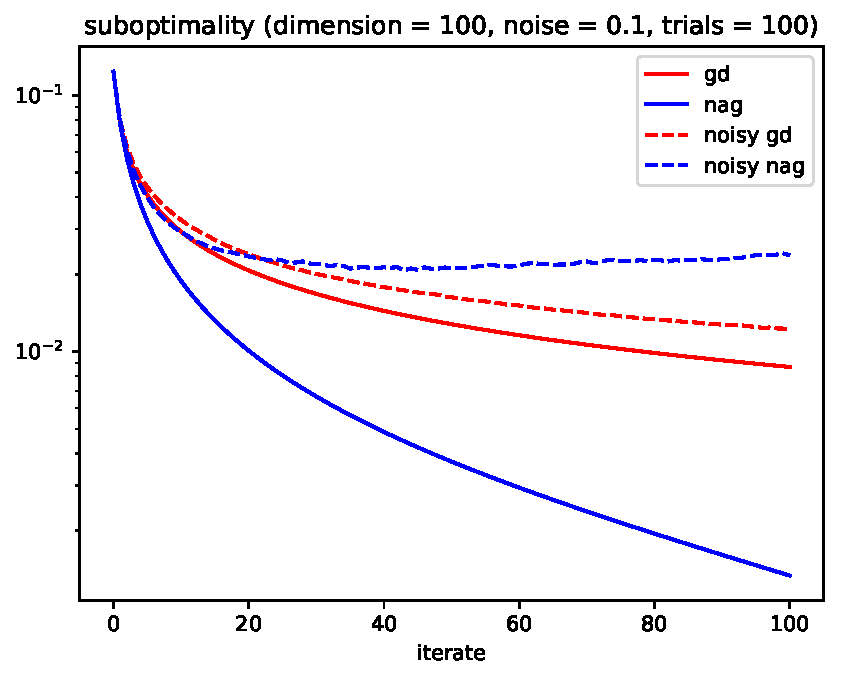
\includegraphics[width=3in]{figures/nag-noise.pdf}
\end{center}
\caption{The optimality gap for iterations of gradient descent and Nesterov accelerated gradient descent applied to the worst function in the world with dimension $n=100$. Notice with exact oracle gradients, acceleration helps significantly. However, when adding uniform spherical random noise with radius $\delta=0.1$ to the gradient, stochastic gradient descent remains robust while stochastic accelerated gradient accumulates error. The stochastic results are averaged over $100$ trials.}
\label{fig:nag-noise}
\end{figure}

The preceeding example is not wickedly pathological in any sense. Instead, it is
illustrative of a much broader phenomenon. Work by Devolder, Glineur and
Nesterov (DGN) \cite{devolder2014first} shows there is a
fundamental trade-off between acceleration and robustness, in a sense
made precise below. 

First, define the notion of an inexact gradient oracle. Recall for a
$\beta$-smooth convex function $f$ and any $x, y \in \domain$,
\begin{align}
    0 \leq f(x)  - \Paren{f(y) + \langle \grad f(y), x - y \rangle}
    \leq \frac{\beta}{2} \norm{x-y}^2. \label{eq:exact-oracle}
\end{align}
For any $y \in \domain$, an exact first-order oracle then returns a pair
$(f(y), g(y)) = (f(y), \grad f(y))$ that satisfies~\eqref{eq:exact-oracle}
exactly for every $x \in \domain$. 
An inexact oracle, returns a pair so that~\eqref{eq:exact-oracle} holds up to some
slack $\delta$.
~
\begin{definition}[Inexact-Oracle]
Let $\delta > 0$. For any $y\in \domain$, a $\delta$-inexact oracle returns a pair
$(f_\delta(y), g_\delta(y))$ such that
\begin{align*}
    0 \leq f(x)  - \Paren{f(y) + \langle \grad f(y), x - y \rangle}
    \leq \frac{\beta}{2} \norm{x-y}^2 + \delta
\end{align*}
for every $x \in \domain$.
\end{definition}
Consider running gradient descent with a $\delta$-inexact oracle.
DGN \cite{devolder2014first} show, after $t$ steps,
\begin{align*}
    f(x_t) - f(x^\star) \leq \frac{\beta R^2}{2t} + \delta.
\end{align*}
Comparing this rate with Table~\eqref{table:upper-bounds}, the plain gradient
method is not affected by the inexact oracle and doesn't accumulate errors. 
On the other hand, if the accelerated gradient
method is run with a $\delta$-inexact oracle, then after $t$ steps,
\begin{align*}
    f(x_t) - f(x^\star)  \leq \frac{4 \beta R^2}{(t+1)^2} +
    \frac{1}{3}(t+3)\delta.
\end{align*}
In other words, the accelerated gradient method accumulates errors linearly with
the number of steps! Moreover, this slack is not an artifact of the analysis.
Any black-box method must accumulate errors if it is accelerated in the exact
case, as the following theorem makes precise.
\begin{theorem}[\cite{devolder2014first} Theorem 6]
Consider a black-box method with convergence rate $O\Paren{\frac{\beta R^2}{t^p}}$
when using an exact oracle. With a $\delta$-inexact oracle, suppose the
algorithm achieves a rate
\begin{align}
    f(x_t) - f(x^\star) \leq O\Paren{\frac{\beta R^2}{t^p}} + O\Paren{t^q \delta},
\end{align}
then $q \geq p-1$.
\end{theorem}
In particular, for any accelerated method has $p > 1$, and consequently $q > 1$
so the method acculumates at least $O(t^{p-1} \delta)$ error with the number of
iterations. 

\part{Stochastic optimization}
\section{Lecture 10: Stochastic optimization}
The goal in stochastic optimization is to 
minimize functions of the form
\[
    f(x) = \E_{z\sim \cD}g(x,z)\,
\]
which have stochastic component given by a distribution~$\cD.$ In the case where
the distribution has finite support, the function can be written as
\[
    f(x) = \frac{1}{m}\sum_{i=1}^m f_i(x)\,.
\]
To solve these kinds of problems, we examine the stochastic gradient descent
method and some if its many applications.

\subsection{The stochastic gradient method}

Following Robbins-Monro \cite{Robbins&Monro:1951}, we define the stochastic
gradient method as follows. 

\begin{definition}[Stochastic gradient method]
The stochastic gradient method starts from a point $x_0\in\domain$ and proceeds
according to the update rule
\begin{equation*}
    x_{t+1} = x_t - \eta_t\nabla f_{i_t}(x_t) 
\end{equation*}
where $i_t\in\{1,\dots,m\}$ is either selected at random at each step, or cycled
through a random permutation of $\{1,\dots,m\}$.
\end{definition}

Either of the two methods for selecting~$i_t$ above, lead to the fact that
\[
    \E\nabla f_{i_t}(x) = \nabla f(x)
\]
This is also true when $f(x)=\E g(x,z)$ and at each step we update according to
$\nabla g(x,z)$ for randomly drawn~$z\sim\cD.$
%
\subsubsection{Sanity check}

Let us check that on a simple problem that the stochastic gradient descent yields the optimum. Let $p_1, \dots, p_m\in \R^n$, and define $f\colon \R^n \rightarrow \R_+$:
\begin{equation*}
    \forall x\in \R^n,\ f(x) = \frac{1}{2m}\sum_{i=1}^m \|x-p_i\|_2^2
\end{equation*}
Note that 
here $f_i(x) = \frac{1}{2}\|x-p_i\|_2^2$ 
and $\nabla f_i(x) = x-p_i.$ 
Moreover,
\begin{equation*}
    x^* = \argmin_{x\in\R^d} f(x) = \frac{1}{m}\sum_{i=1}^mp_i
\end{equation*}

Now, run SGM with $\eta_t=\frac{1}{t}$ in cyclic order i.e. $i_t = t$ and $x_0=0$:
\begin{align*}
    x_0 &= 0 \\
    x_1 &= 0 - \frac{1}{1}(0-p_1) = p_1 \\
    x_2 &= p_1 - \frac{1}{2}(p_1-p_2) = \frac{p_1+p_2}{2}\\
    \vdots\\
    x_n &= \frac{1}{m}\sum_{i=1}^mp_i = x^*
\end{align*}

\subsection{The Perceptron}

The
\href{https://www.nytimes.com/1958/07/08/archives/new-navy-device-learns-by-doing-psychologist-shows-embryo-of.html}{New
York Times} wrote in 1958 that the Perceptron \cite{Rosenblatt58theperceptron:}
was:
\begin{quote}
\emph{the embryo of an electronic computer that [the Navy] expects will be able
to walk, talk, see, write, reproduce itself and be conscious of its existence.}
\end{quote}

So, let's see.

\begin{definition}[Perceptron] 
Given labeled points~$((x_1, y_1),\dots,(x_m,y_m))\in(\R^n\times\{-1,1\})^m,$ 
and and initial point~$w_0\in\R^n$, the Perceptron is the following algorithm. 
For $i_t\in\{1,\dots,m\}$ selected uniformly at random,
\begin{equation*}
w_{t+1} =w_t(1-\gamma) + \eta \begin{cases}
    y_{i_t}x_{i_t}& \text{if } y_{i_t}\langle w_t, x_{i_t}\rangle <1\\
    0              & \text{otherwise}
\end{cases}
\end{equation*}
\end{definition}

Reverse-engineering the algorithm, the Perceptron is equivalent to running the
SGM on the Support Vector Machine (SVM) objective function.

\begin{definition}[SVM] 

Given labeled points~$((x_1, y_1),\dots,(x_m,y_m))\in(\R^n\times\{-1,1\})^m,$ 
the SVM objective function is:
\begin{equation*}
    f(w) = \frac{1}{n}\sum_{i=1}^m \max(1-y_i\langle w, x_i\rangle,\; 0) + \lambda \|w\|_2^2
\end{equation*}
The loss function $\max(1-z,\;0)$ is known as the Hinge Loss. The extra 
term~$\lambda \|w\|_2^2$ is known as the regularization term.
\end{definition}

\subsection{Empirical risk minimization}
We have two spaces of objects $\mathcal{X}$ and ${\mathcal{Y}},$ where we think
of $\mathcal{X}$ as the space of \emph{instances} or \emph{examples}, and
$\mathcal{Y}$ is a the set of \emph{labels} or \emph{classes}.

Our goal is to \emph{learn} a function $h\colon\mathcal{X}\to\mathcal{Y}$ which
outputs an object $y\in \mathcal{Y}$, given $ x\in \mathcal{X}$.  Assume there
is a joint distribution $\mathcal{D}$ over the space~$\mathcal{X} \times
\mathcal{Y}$ and the training set consists of $m$ instances $(x_1, y_1), \ldots,
(x_m,y_m)$ drawn i.i.d.~from $\mathcal{D}$.

We also define a non-negative real-valued loss function $\ell(y^\prime,y)$ to
measure the difference between the prediction $y^\prime$ and the true outcome
$y$.

\begin{definition}
The risk associated with h(x) is defined as the expectation of the loss function:
\begin{equation*}
    R[h] = \mathbb{E}_{\mathcal{X} \times \mathcal{Y} \in \mathcal{D}} \ell(h(x),y)
\end{equation*}
\end{definition}
The ultimate goal of a learning algorithm is to find $h^*$ among a class of functions $\mathcal{H}$ that minimizes $R[h]$:
\begin{equation*}
    h^* = \text{arg}\min_{h \in \mathcal{H}} R[h]
\end{equation*}
In general, the risk $R[h]$ can not be computed because the joint distribution is unknown. Therefore,

The \emph{empirical risk} is defined by averaging the loss function of the training set:
\begin{equation*}
    R_n[h] = \frac{1}{n} \sum^n_{i=1}\ell(h(x_i),y_i)
\end{equation*}
An empirical risk minimizer is any point $h^* \in \arg\min_{h \in \mathcal{H}} R_n[h]$.

The stochastic gradient method can be thought of as minimizing the risk
directly, if each example is only used once. In cases where we make multiple
passes over the training set, it is better to think of it as minimizing the
empirical risk, which can give different solutions than minimizing the risk.
We'll develop tools to relate risk and empirical risk in the next lecture.

\subsection{Online Learning}

An interesting variant of this learning setup is called \emph{online learning}.
It arises when we do not have a set of training data, but rather must make
decisions one-by-one.

\paragraph{Taking advice from experts.}
Imagine we have access to the predictions of $n$ experts. 
We start from an initial distribution over experts, given by
weights~$w_1\in\Delta_n = \{ w\in\R^n\colon \sum_i w_i=1, w_i\ge0\}.$

At each step $t = 1, \ldots, T$:
\begin{itemize}
    \item we randomly choose an expert according to~$w_t$
    \item nature deals us a loss function $f_t\in[-1,1]^n,$ specifying for each
expert~$i$ the loss~$f_t[i]$ incurred by the prediction of expert~$i$ at
time~$t.$
    \item we incur the expected loss $\E_{i\sim w_t}f_t[i]=\langle
w_t,f_t\rangle.$
    \item we get to update our distribution to from $w_t$ to $w_{t+1}.$
\end{itemize}

At the end of the day, we measure how well we performed relative to the best
fixed distribution over experts in hindsight. This is called \emph{regret}:
\begin{equation*}
   R = \sum^T_{t = 1} \langle w_{t}, f_t \rangle - \min_{w \in \Delta_n} \sum^{T}_{t = 1} \langle w, f_t \rangle
\end{equation*}
This is a relative benchmark. Small regret does not say that the loss is necessarily
small. It only says that had we played the same strategy at all steps, we
couldn't have done much better even with the benefit of hindsight.

Perhaps the most important online learning algorithm is the \emph{multiplicative
weights update} given by the following simple update rule:
\begin{align*}
    v_t[i] &= w_{t-1}[i]e^{-\eta f_t[i]} \tag{exponential weights update}\\
    w_t &= v_t/(\textstyle\sum_i v_t[i]) \tag{normalize}
\end{align*}
The question is \textit{how do we bound the regret} of the multiplicative
weights update? We could do a direct analysis, but instead we'll relate
multiplicative weights to gradient descent and use the convergence guarantees
we already know.

\subsection{Multiplicative weights as mirror descent}

Recall that mirror descent requires a mirror map $\phi : \Omega \to R$ over a
domain $\Omega \in \mathbb{R}^n$ where $\phi$ is strongly convex and
continuously differentiable.

The associated projection is
\begin{equation*}
    \Pi^\phi_\domain (y) = \argmin_{x\in\domain} \mathcal{D}_\phi(x,y)
\end{equation*}
where $\mathcal{D}_\phi(x,y)$ is Bregman divergence.
\begin{definition}
The Bregman divergence measures how good the first order approximation of the
function~$\phi$ is:
    \begin{equation*}
        \mathcal{D}_\phi(x,y) = \phi(x) - \phi(y) - \nabla \phi(y) ^\intercal (x-y)
    \end{equation*}
\end{definition}
The mirror descent update rule is:
\begin{align*}
    \nabla \phi(y_{t+1}) &= \nabla \phi (x_t) - \eta g_t \\
    x_{t+1} &=  \Pi^\phi_\domain (y_{t+1})
\end{align*}
where $g_t \in \partial f(x_t).$ 
In the first homework, we proved the following results.
\begin{theorem}
    let $\|\cdot\|$ be arbitrary norm and suppose that $\phi$ is $\alpha$-strongly convex      \textbf{w.r.t.} $\|\cdot\|$ on $\domain$. Suppose that $f_t$ is $L$-lipschitz \textbf{w.r.t.} $\|\cdot\|$, we have:
    \begin{equation*}
        \frac{1}{T}\sum^T_{t=1} f_t(x_t) \leq \frac{ \mathcal{D}_\phi(x^*,x_0)}{T \eta}+ \eta \frac{L^2}{2\alpha}
    \end{equation*}
\end{theorem}


Multiplicative weights are an instance of the Mirror Descent where $\Phi: w\mapsto \sum_{i=1}^m w_i \log(w_i)$.

Note that $\nabla\Phi : w\mapsto 1 + \log(w)$ where the log is taken elementwise.
The update rule in Mirror Descent becomes:
\begin{align*}
    \nabla\Phi(v_{t+1}) &=\nabla\Phi(w_{t}) - \eta_tf_t \\
    \implies v_{t+1} &= w_te^{-\eta_t f_t}
\end{align*}

Now comes the projection step. The Bregman divergence is, for all $(x,y)\in\domain^2$:
\begin{align*}
    D_{\Phi}(x,y) &= \Phi(x)-\Phi(y) - \nabla\Phi(y)^T(x-y)
\end{align*}
yielding for all $y$:
\begin{align*}
    \Pi_{\domain}^{\Phi}(y) = \argmin_{x\in\domain}D_{\Phi}(x,y)
\end{align*}

\section{Lecture 11: Learning, Stability, Regularization
}

In this lecture we take a look at machine learning, and empirical risk
minimization in particular. We define the distribution of our data as $D$ over
$X\times Y$, where $X\subseteq \R^{d}$ and $Y$ is some discrete set of class
labels. For instance, in a binary classification tasks with two labels $Y$ 
might be $ Y = \{ -1,1 \}$.
\begin{itemize}
\item A ``model'' is specified by a set of parameters $w \in
\domain\subseteq\mathbb{R}^n$
\item The ``loss function'' is denoted by $\ell\colon \domain \times (X\times Y)
\rightarrow \R$, note that $\ell(w,z)$ gives the loss of model $w$ on instance
$z.$
\item The risk of a model is defined as $R(w)=\E_{z\sim D}[\ell(w,z)].$
\end{itemize}
Our goal is to find a model~$w$ that minimizes~$R(w).$

One way to accomplish this is to use stochastic optimization directly on the
population objective:
$$w_{t+1} = w_{t} - \eta \nabla \ell(w_t,z_t) \quad z\sim D$$

When given a finite data set, however, it is usually effective to make multiple
passes over the data. In this case, the stochastic gradient method may no longer
optimize risk directly.
%
\subsection{Empirical risk and generalization error}

Consider a finite sample Suppose $S=((x_1,y_1),......,(x_m,y_m))\in(X\times
Y)^m$, where $z_i=(x_i,y_i)$ represents the $i$-th labeled example.
The empirical risk is defined as
\[
R_{S}(w) = \frac{1}{m}\sum_{i=1}^{m}\ell(w,z_i)\,.
\]
Empirical risk minimization is commonly used as a proxy for minimizing the
unknown population risk. But how good is this proxy? Ideally, we would like that
the point~$w$ that we find via empirical risk minimization has $R_S(w)\approx
R(w).$ However, this may not be the case, since the risk $R(w)$ captures loss on
unseen example, while the empirical risk $R_S(w)$ captures loss on seen
examples. Generally, we expect to do much better on seen examples than unseen
examples. This performance gap between seen and unseen examples is what we call
\emph{generalization error}.

\begin{definition}[Generalization error]
We define the \emph{generalization error} of a model~$w$ as
$$\epsilon_{\text{gen}}(w) = R(w) - R_{s}(w)\,.$$
\end{definition}
Note the following tautological, yet important identity:
\begin{equation}
R(w) = R_{S}(w) + \epsilon_{\text{gen}}(w)
\end{equation} 
What this shows in particular is that if we manage to make the empirical risk
$R_S(w)$ small through optimization, then all that remains to worry about is
generalization error.

So, how can we bound generalization error? The fundamental relationship we'll
establish in this lecture is that generalization error equals an algorithmic
robustness property that we call \emph{algorithmic stability}. Intuitively,
algorithmic stability measures how sensitive an algorithm is to changes in a
single training example.

\subsection{Algorithmic stability}

To introduce the idea of stability, we choose two independent samples
$S = (z_1, ... , z_m)$ and $S^{\prime} = (z^{\prime}_1, ... ,z^{\prime}_{m})$,
each drawn independently and identically from~$D$. Here, the second sample $S'$
is called a \emph{ghost sample} and mainly serves an analytical purpose.

Correlating the two samples in a single point, we introduce the hybrid sample
$S^{(i)}$ as:
$$S^{(i)} = (z_1, \,... ,\, z_{i-1}, \,z_{i}^{\prime},\, z_{i+1}, \,... \,,z_{m})$$
Note that here the $i$-th example comes from~$S',$ while all others come
from~$S.$

With this notation at hand, we can introduce a notion of average stability.
\begin{definition}[Average stability] 
The \emph{average stability} of an algorithm $A: (X \times Y)^{m} \rightarrow \domain$:
$$\Delta(A) = \E_{S,
S^{\prime}}\left[\frac{1}{m}\sum_{i=1}^{m}\left(\ell(A(S),z_i^{\prime}) -
\ell(A(S^{(i)}),z_{i}^{\prime})\right)\right]$$
\end{definition}
This definition can be interpreted as comparing the performance of the algorithm 
on an unseen versus a seen example. This is the intuition why average stability,
in fact, equals generalization error.
\begin{theorem}
$$\E[\epsilon_{\text{gen}}(A)] = \Delta(A)$$
\end{theorem}
\begin{proof}
Note that
\begin{align*}
\E[\epsilon_{\text{gen}}(A)] &= R(A(S)) - R_{S}(A(S))\,, \\
\E\left[R_{S}(A(S))\right]] &=
\E\left[\frac{1}{m}\sum_{i=1}^{m}\ell(A(S),z_i)\right]\,,\\
\E [R(A(S))]&=
\E\left[\frac{1}{m}\sum_{i=1}^{m}\ell(A(S),z_i^{\prime})\right]\,.
\end{align*}
At the same time, since $z_i$ and $z_i'$ are identically distributed and
independent of the other examples, we have
\[
\E\ell(A(S),z_i) = \E\ell(A(S^{(i)}),z_i^{\prime})\,.
\]
Applying this identity to each term in the empirical risk above, and comparing
with the definition of $\Delta(A),$ we conclude
$\E[R(A(S)) - R_S(A(S))] = \Delta(A)$
\end{proof}

\subsubsection{Uniform stability}
%
While average stability gave us an exact characterization of generalization
error, it can be hard to work with the expectation over $S$ and $S'.$ Uniform
stability replaces the averages by suprema, leading to a stronger but useful
notion~\cite{BousquettE02}.
%
\begin{definition}[Uniform stability]
The uniform stability of an algorithm $A$ is defined as 
\begin{equation*}
\Delta_{\sup}(A) = \sup_{\mathcal{S}, \mathcal{S}' \in (X\times Y)^m } 
\sup_{i \in [m]} |\ell(A(S), z_i') - \ell(A(S^{(i)}, z_i')|
\end{equation*}
\end{definition}

Since uniform stability upper bounds average stability, we know that uniform
stability upper bounds generalization error (in expectatation).
%
\begin{corollary}
$\E[\epsilon_{\text{gen}}(A)] \leq \Delta_{\sup} (A)$
\end{corollary}

This corollary turns out to be surprisingly useful since many algorithms are
uniformly stable. For instance, strongly convex loss function is sufficient for
stability, and hence generalization as we will show next.

\subsection{Stability of empirical risk minimization}

The next theorem due to~\cite{Shalev2010LearnabilitySA} shows that empirical
risk minimization of a strongly convex loss function is uniformly stable.

\begin{theorem}
Assume $\ell(w, z)$ is $\alpha$-strongly convex over the domain~$\domain$
and $L$-Lipschitz. 
Let $\hat w_S = \arg \min_{w\in \domain} \frac{1}{m} \sum_{i=1}^m \ell(w, z_i)$
denote the empirical risk minimizer (ERM).
Then, ERM satisfies
\begin{equation*}
\Delta_{\sup} (\text{ERM}) \leq \frac{4L^2}{\alpha m}\,.
\end{equation*}
\end{theorem}

An interesting point is that there is no explicit reference to the complexity of
the class. In the following we present the proof.

\begin{proof}
Denote by $\hat w_S$ the empirical risk minimizer on a sample~$S.$
Fix arbitrary samples $S,S'$ of size $m$ and an index $i\in[m].$
We need to show that 
\[
|( \ell(\hat w_{S^{(i)}}, z_i') - \ell(\hat w_{S}, z_i')) |  \leq \frac{4
L^2}{\alpha m}\,.
\]
On one hand, by strong convexity we know that
\[
R_S(\hat w_{S^{(i)}}) - R_S(\hat w_{S}) \geq \frac{\alpha}{2} \| \hat w_{S} -
\hat w_{S^{(i)}} \|^2 \,.
\]
On the other hand, 
\begin{align*}
& R_S(\hat w_{S^{(i)}}) - R_S(\hat w_{S})\\
&=  \frac{1}{m} ( \ell(\hat w_{S^{(i)}}, z_i) - \ell(\hat w_{S}, z_i)) + \frac{1}{m} \sum_{i \neq j} ( \ell(\hat w_{S^{(i)}}, z_j) - \ell(\hat w_{S}, z_j))\\
&=\frac{1}{m} (\ell(\hat w_{S^{(i)}}, z_i) - \ell(\hat w_{S}, z_i)) 
+ \frac{1}{m} (\ell(\hat w_{S}, z_i') - \ell(\hat w_{S^{(i)}}, z_i')) 
+ \left(R_{S^{(i)}}(\hat w_{S^{(i)}}) - R_{S^{(i)}}(\hat w_{S})\right)\\ 
&\leq \frac{1}{m} | \ell(\hat w_{S^{(i)}}, z_i) - \ell(\hat w_{S}, z_i)| +
\frac{1}{m} | ( \ell(\hat w_{S}, z_i') - \ell(\hat w_{S^{(i)}}, z_i')) | \\
&\leq  \frac{2 L}{m} \| \hat w_{S^{(i)}} - \hat w_{S}\|\,.
\end{align*}
Here, we used that 
\[
R_{S^{(i)}}(\hat w_{S^{(i)}}) - R_{S^{(i)}}(\hat w_{S})) \leq 0
\]
and the fact that $\ell$ is $L-$lipschitz.

Putting it all together $\| \hat w_{S^{(i)}} - \hat w_{S} \| \leq \frac{4 L}{\alpha m}$. Then by the Lipschitz condition we have that 
\[
\frac{1}{m} | ( \ell(\hat w_{S^{(i)}}, z_i') - \ell(\hat w_{S}, z_i')) | \leq L
\| \hat w_{S^{(i)}} - \hat w_{S} \| \leq \frac{4 L ^ 2}{\alpha m}\,.
\]
Hence, $\Delta_{\sup}(\text{ERM}) \leq \frac{4 L ^ 2}{\alpha m}$.

\end{proof}


\subsection{Regularization}

Not all the ERM problems are strongly convex. However, if the problem is convex we can consider the regularized objective
\begin{equation*}
r(w, z) = \ell(w, z) + \frac{\alpha}{2} \| w \|^2
\end{equation*}

The regularized loss $r(w, z)$ is $\alpha-$strongly convex. The last term is
named $\ell_2$-regularization, weight decay or Tikhonov regularization depending on
the field you work on. Therefore, we now have the following chain of
implications: 
$$
\text{regularization} \Rightarrow \text{strong convexity} \Rightarrow \text{uniform stability} \Rightarrow \text{generalization}
$$

We can also show that solving the regularized objective also solves the
unregularized objective. Assume that $\domain \subseteq \mathcal{B}_2(R)$, by
setting $\alpha \approx \frac{L^2}{R^2 m}$ we can show that the minimizer of the
regularized risk also minimizes the unregularized risk up to error
$\mathcal{O}(\frac{LR}{\sqrt{m}})$. Moreover, by the previous theorem the
generalized error will also be $\mathcal{O}(\frac{LR}{\sqrt{m}})$. See Theorem~3
in~\cite{Shalev2010LearnabilitySA} for details.

\subsection{Implicit Regularization}

In implicit regularization the algorithm itself regularizes the objective, instead of explicitly adding a regularization term. The following theorem describes the regularization effect of the Stochastic Gradient Method (SGM). 

\begin{theorem}Assume $\ell(\cdot, z)$ is convex, $\beta$-smooth and $L$-Lipschitz. If we run SGM for T steps, then the algorithm has uniform stability
\begin{equation*}
\Delta_{\sup}(\text{SGM}_T) \leq \frac{2 L^2}{m} \sum_{t=1}^T \eta_t
\end{equation*}
\end{theorem}
Note for $\eta_t \approx \frac{1}{m}$ then $\Delta_{\sup}(\text{SGM}_T) = \mathcal{O}(\frac{\log(T)}{m})$, and for $\eta_t \approx \frac{1}{\sqrt{m}}$ and $T=\mathcal{O}(m)$ then $\Delta_{\sup}(\text{SGM}_T) = \mathcal{O}(\frac{1}{\sqrt{m}} )$. See \cite{HardtRS15} for proof.

%!TEX root = max_main.tex
\section{Lecture 12: Coordinate Descent}
There are many classes of functions for which it is very cheap 
to compute directional derivatives along the standard basis vectors
$e_i, i \in [n]$.
%
For example, 
%
\begin{eqnarray}
f(x) = \|x\|^2\quad \text{ or }\quad f(x) = \|x\|_1
\end{eqnarray}
%
This is especially true of common regularizers, 
%
which often take the form 
\begin{eqnarray}
R(x) = \sum_{i=1}^n R_i(x_i) \ .
\end{eqnarray}
%
More generally, many objectives and regularizes exhibit ``group sparsity''; that is,
%
\begin{eqnarray}
R(x) =  \sum_{j=1}^m R_{j}(x_{S_j})
\end{eqnarray}
where each $S_j, j \in [m]$ is a subsect of $[n]$, and similarly for $f(x)$.
%
Examples of functions with block decompositions and group sparsity include:
\begin{enumerate} 
	\item Group sparsity penalties;
	\item Regularizes of the form $R(U^\top x)$, where $R$ is
    coordinate-separable, and $U$ has sparse columns and so
    $(U^\top x) = u_i^\top x$ depends only on the nonzero entries of $U_i$;
	\item Neural networks, where the gradients with respect to some weights can be
    computed ``locally''; and
	\item ERM problems of the form 
    \begin{eqnarray}
    f(x) := \sum_{i=1}^n \phi_i(\langle w^{(i)} , x \rangle )
    \end{eqnarray}
    where $\phi_i: \R \to \R$, and $w^{(i)}$ is zero except in a few coordinates. 
\end{enumerate} 

% Code the produce the figure below
\begin{figure}[t]
\centering
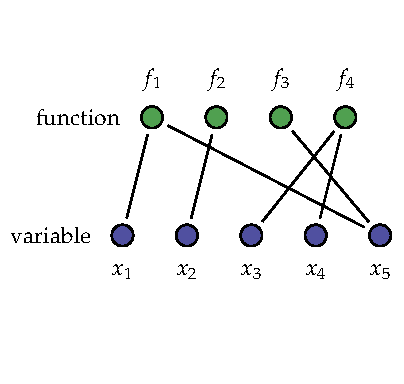
\includegraphics{figures/lecture12-function_coordinate_graph.pdf}

%\definecolor{myblue}{RGB}{80,80,160}
%\definecolor{mygreen}{RGB}{80,160,80}
%\usetikzlibrary{positioning,chains,fit,shapes,calc}
%
%\begin{tikzpicture}[thick,
%  every node/.style={draw,circle},
%  fsnode/.style={fill=myblue},
%  ssnode/.style={fill=mygreen},
%  every fit/.style={draw=none},
%  shorten >= 3pt,shorten <= 3pt
%]
%
%% Function
%\begin{scope}[start chain=going right,node distance=7mm]
%\foreach \i in {1,2,...,5}
%  \node[fsnode,on chain] (x\i) [label=below: $x_\i$] {};
%\end{scope}
%\node [myblue,fit=(x1) (x5),label=left:variable] {};
%
%% Coordinates
%\begin{scope}[yshift=2cm,xshift=.5cm,start chain=going right,node distance=7mm]
%\foreach \i in {1,2,...,4}
%  \node[ssnode,on chain] (f\i) [label=above: $f_\i$] {};
%\end{scope}
%\node [mygreen,fit=(f1) (f4),label=left:function] {};
%
%% Edges
%\draw (x1) -- (f1);
%\draw (x2) -- (f2);
%\draw (x3) -- (f4);
%\draw (x4) -- (f4);
%\draw (x5) -- (f1);
%\draw (x5) -- (f3);
%\end{tikzpicture}
\vspace{-20pt}
\caption{
  Example of the bipartite graph between component functions
  $f_i, i \in [m]$ and variables $x_j, j \in [n]$ induced by the
  group sparsity structure of a function $f : \R^n \to \R^m$.
  An edge between $f_i$ and $x_j$ conveys that the $i$th component function
  depends on the $j$th coordinate of the input.
}
\end{figure}

\subsection{Coordinate Descent}
  Denote $\partial_i f= \frac{\partial f}{x_i}$.
  For each round $t = 1,2,\dots$, the coordinate descent algorithm
  chooses an index $i_t \in [n]$, and computes
	\begin{eqnarray}
	x_{t+1} = x_t - \eta_t\partial_{i_t}f(x_t) \cdot e_{i_t} \ .
	\end{eqnarray}
  This algorithm is a special case of stochastic gradient descent. For
	\begin{eqnarray}
    \E[x_{t+1} | x_t]
    &=& x_t - \eta_t \E [\partial_{i_t}f(x_t) \cdot e_{i_t}] \\
    &=& x_t - \frac{\eta_t}{n} \sum_{i=1}^n \partial_{i}f(x_t) \cdot e_i \\
    &=& x_t - \eta_t \nabla f(x_t) \ .
	\end{eqnarray}
	Recall the bound for SGD: If $\E[g_t] = \nabla f(x_t)$, then SGD with step size $\eta = \frac{1}{BR}$ satisfies
	\begin{eqnarray}
	\E[f(\frac{1}{T}\sum_{t=1}^T x_t)] - \min_{x \in \Omega}f(x) \le \frac{2 BR}{\sqrt{T}}
	\end{eqnarray}
	where $R^2$ is given by $\max_{x \in \Omega} \|x-x_1\|^2_2$ and $B = \max_{t}\E[\|g_t\|^2_2]$. In particular, if we set $g_t = n \partial_{x_{i_t}}f(x_t) \cdot e_{i_t}$, we compute that
	\begin{eqnarray}
    \E[\|g_t\|^2_2]
    = \frac{1}{n} \sum_{i=1}^n \|n\cdot \partial_{x_{i}}f(x_t) \cdot e_i\|^2_2
    = n \|\nabla f(x_t)\|^2_2 \ .
	\end{eqnarray}
	If we assume that $f$ is $L$-Lipschitz, we additionally have that 
	$\E[\|g_t\|^2] \le nL^2$.
  This implies the first result:
	\begin{proposition} Let $f$ be convex and $L$-Lipschitz on $\R^n$.
    Then coordinate descent with step size $\eta = \frac{1}{n R}$ has convergence rate 
	\begin{eqnarray}
	\E[f(\frac{1}{T}\sum_{t=1}^T x_t)] - \min_{x \in \Omega}f(x) \le 2LR\sqrt{n/T}
	\end{eqnarray}
	\end{proposition}
	\subsection{Importance Sampling}
	In the above, we decided on using the uniform distribution to sample a
  coordinate. But suppose we have more fine-grained information. In particular, what if we knew that we could bound $\sup_{x \in \Omega} \|\nabla f(x)_i\|_2 \le L_i$? An alternative might be to sample in a way to take $L_i$ into account. This motivates the ``importance sampled'' estimator of $\nabla f(x)$, given by
	\begin{eqnarray}
	g_t = \frac{1}{p_{i_t}} \cdot \partial_{i_t}f(x_{t}) \text{ where } i_t \sim
    \mathrm{Cat}(p_1,\dots,p_n) \ .
	\end{eqnarray}
	Note then that $\E[g_t] = \nabla f(x_t)$, but
	\begin{eqnarray}
    \E[\|g_t\|^2_2]
    &=& \sum_{i=1}^n (\partial_{i_t}f(x_{t}))^2/p_i^2\\
    &\le& \sum_{i=1}^n L_i^2/p_i^2
	\end{eqnarray}
	In this case, we can get rates 
	\begin{eqnarray}
	  \E[f(\frac{1}{T}\sum_{t=1}^T x_t)] - \min_{x \in \Omega}f(x)
    \le 2R\sqrt{1/T}\cdot \sqrt{\sum_{i=1}^n L_i^2/p_i^2}
	\end{eqnarray}
	In many cases, if the values of $L_i$ are heterogenous, we can optimize the values of $p_i$. 
	\subsection{Importance Sampling For Smooth Coordinate Descent}
	In this section, we consider coordinate descent with a \emph{biased}
  estimator of the gradient. Suppose that we have, for $x \in \R^n$
  and $\alpha \in \R$, the inequality
	\begin{eqnarray}
    |\partial_{x_i} f(x) - \partial_{x_i} f(x + \alpha e_i)|
    \le \beta_{i}|\alpha|
	\end{eqnarray}
	where $\beta_i$ are possibly heterogenous. Note that if that $f$ is twice-continuously differentiable, the above condition is equivalent to $\nabla^2_{ii}f(x) \le \beta_i$, or $\mathrm{Diag}(\nabla^2 f(x)) \preceq \mathrm{diag}(\boldsymbol{\beta})$.  Define the distribution $p^\gamma$ via
	\begin{eqnarray}
	p^{\gamma}_i = \frac{\beta_i^{\gamma}}{\sum_{j=1}^n \beta_j^{\gamma}}
	\end{eqnarray}
	We consider gradient descent with the rule called $\mathrm{RCD}(\gamma)$
	\begin{eqnarray}\label{RCDgamma}
    x_{t+1} = x_t - \frac{1}{\beta_{i_t}} \cdot \partial_{i_t}(x_t) \cdot e_{i_t}, \text{ where } i_t \sim p^{\gamma}
	\end{eqnarray}
  Note that as $\gamma \to \infty$, coordinates with larger values of $\beta_i$
  will be selected more often.
	Also note that this is \emph{not generally} equivalent to SGD, because 
	\begin{eqnarray}
    \E\left[\frac{1}{\beta_{i_t}}\partial_{i_t}(x_t)e_i\right]
    = \frac{1}{\sum_{j=1}^n \beta_j^{\gamma}} \cdot \sum_{i=1}^n \beta_{i}^{\gamma - 1} \partial_i f(x_t)e_i
    = \frac{1}{\sum_{j=1}^n \beta_j^{\gamma}} \cdot \nabla f(x_t) \circ (\beta_i^{\gamma - 1})_{i \in [n]}
	\end{eqnarray}
	which is only a scaled version of $\nabla f(x_t)$ when $\gamma = 1$. Still, we can prove the following theorem:
	\begin{theorem}
  \label{thm:6.7}
  Define the weighted norms
	\begin{eqnarray}
	\|x\|_{[\gamma]}^2 := \sum_{i=1}^n x_i^2 \beta_i^\gamma \text{ and } \|x\|_{[\gamma]}^{*2} := \sum_{i=1}^n x_i^2 \beta_i^{-\gamma}
	\end{eqnarray}
	and note that the norms are dual to one another.
  We then have that the rule $\mathrm{RCD}(\gamma)$ produces iterates satisfying
	\begin{eqnarray}
	  \E[f(x_t) - \arg\min_{x \in \R^{n}} f(x)]
    \le \frac{2 R^2_{1-\gamma} \cdot \sum_{i=1}^n \beta_{i}^{\gamma}}{t-1}~,
	\end{eqnarray}
	where $R^2_{1-\gamma} = \sup_{x \in \R^n:f(x) \le f(x_1)} \|x - x^*\|_{[1 - \gamma]}$.
	\end{theorem}
	\begin{proof}
	Recall the inequality that for a general $\beta_g$-smooth convex function $g$, one has that
	\begin{eqnarray}
    g\left(u - \frac{1}{\beta_g}\nabla g(u)\right) - g(u)
    \le -\frac{1}{2\beta_g} \|\nabla g\|^2
	\end{eqnarray}
	Hence, considering the functions $g_i(u;x) = f(x + ue_i)$, we see that $\partial_i f(x) = g_i'(u;x)$, and thus $g_i$ is $\beta_i$ smooth. Hence, we have 
	\begin{eqnarray}
    f\left(x - \frac{1}{\beta_i}\nabla f(x)e_i\right) - f(x)
    = g_i(0 - \frac{1}{\beta_g}g_i'(0;x)) - g(0;x)
    \le -\frac{g_i'(u;x)^2}{2\beta_i} = - \frac{\partial_i f(x)^2}{2\beta_i} \ .
	\end{eqnarray}
	Hence, if $i~p^\gamma$, we have
	\begin{eqnarray}
	  \E[f(x - \frac{1}{\beta_i}\partial_i f(x)e_i) - f(x)]
    &\le& \sum_{i=1}^n p_i^\gamma \cdot - \frac{\partial_i f(x)^2}{2\beta_i}\\
	  &=& -\frac{1}{2\sum_{i=1}^n \beta_i^{\gamma}} \sum_{i=1}^n \beta^{\gamma - 1}\partial_i f(x)^2 \\
	  &=& -\frac{\|\nabla f(x)\|^{*2}_{[1-\gamma]})}{2\sum_{i=1}^n \beta_i^{\gamma}}
	\end{eqnarray}
	Hence, if we define $\delta_t = \E[f(x_t) - f(x^*)]$, we have that
	\begin{eqnarray}
	\delta_{t+1} - \delta_t \le -\frac{\|\nabla f(x_t)\|^{*2}_{[1-\gamma]}}{2\sum_{i=1}^n \beta_i^{\gamma}} 
	\end{eqnarray}
	Moreover, with probability $1$, one also has that $f(x_{t+1}) \le f(x_t)$, by the above. We now continue with the regular proof of smooth gradient descent. Note that
	\begin{eqnarray*}
	\delta_t &\le& \nabla f(x_t)^\top(x_t - x_*)\\
	&\le& \|\nabla f(x_t)\|_{[1-\gamma]}^*\|x_t - x_*\|_{[1-\gamma]}\\
	&\le& R_{1-\gamma}\|\nabla f(x_t)\|_{[1-\gamma]}^*\ .
	\end{eqnarray*}
	Putting these things together implies that
	\begin{eqnarray}
	\delta_{t+1} - \delta_t \le -\frac{\delta_t^2}{2R_{1-\gamma}^2\sum_{i=1}^n \beta_i^{\gamma}} 
	\end{eqnarray}
	Recall that this was the recursion we used to prove convergence in the non-stochastic case.
	\end{proof}
	\begin{theorem} If $f$ is in addition $\alpha$-strongly convex w.r.t to $\|\cdot\|_{[1-\gamma]}$, then we get 
	\begin{eqnarray}
    \E[f(x_{t+1}) - \arg\min_{x \in \R^{n}} f(x)]
    \le \left(1 - \frac{\alpha}{\sum_{i=1}^n \beta_i^\gamma}\right)^t (f(x_1) - f(x^*)) \ .
	\end{eqnarray}
	\end{theorem}
	\begin{proof} We need the following lemma:
  \begin{lemma}
    \label{lemma:6.9} 
    Let $f$ be an $\alpha$-strongly convex function w.r.t to a norm
    $\|\cdot\|$. Then, $f(x) - f(x^*) \le \frac{1}{2\alpha} \|\nabla
    f(x)\|_*^2$\ .
	 \end{lemma}
	 \begin{proof}
	 \begin{eqnarray*}
     f(x) - f(y)
     &\le& \nabla f(x)^\top (x -y ) - \frac{\alpha}{2}\|x - y\|^2_2\\
	   &\le& \|\nabla f(x)\|_* \|x - y\|^2 - \frac{\alpha}{2}\|x - y\|^2_2\\
	   &\le& \max_t \|\nabla f(x)\|_* t - \frac{\alpha}{2}t^2\\
	 	 &=&  \frac{1}{2\alpha} \|\nabla f(x)\|_*^2 \ .
	 \end{eqnarray*}
	 \end{proof}

   Lemma \ref{lemma:6.9} shows that 
	 \begin{eqnarray*}
     \|\nabla f(x_s)\|^{*2}_{[1-\gamma]}
     \ge 2 \alpha \delta_s \ .
	 \end{eqnarray*}
   On the other hand, Theorem \ref{thm:6.7} showed that
   \begin{eqnarray}
   \delta_{t+1} - \delta_t \le -\frac{\|\nabla f(x_t)\|^{*2}_{[1-\gamma]}}{2\sum_{i=1}^n \beta_i^{\gamma}} 
   \end{eqnarray}
   Combining these two, we get
	 \begin{eqnarray}
     \delta_{t+1} - \delta_t &\le& -\frac{\alpha \delta_t}{\sum_{i=1}^n \beta_i^{\gamma}}  \\
     \delta_{t+1} &\le&  \delta_t \left(1  -\frac{\alpha}{\sum_{i=1}^n \beta_i^{\gamma}} \right)~.
	 \end{eqnarray}
   Applying the above inequality recursively and recalling that
   $\delta_t = \E[f(x_t) - f(x^*)]$ gives the result.

	\end{proof}

	\subsection{Random Coordinate vs.\ Stochastic Gradient Descent}
	What's surprising is that $\mathrm{RCD}(\gamma)$ is a descent method, despite being random. This is not true of normal SGD. 
	But when does $\mathrm{RCD}(\gamma)$ actually do better? If $\gamma = 1$, the savings are proportional to the ratio of $\sum_{i=1} \beta_i / \beta \cdot (T_{coord}/T_{grad})$. When $f$ is twice differentiable, this is the ratio of 
	\begin{eqnarray}
	\frac{\tr(\max_{x} \nabla^2 f(x))}{\|\max_{x} \nabla^2 f(x)\|_{\op}} (T_{coord}/T_{grad})
	\end{eqnarray}
	\subsection{Other Extensions to Coordinate Descent}
	\begin{enumerate}
		\item Non-Stochastic, Cyclic SGD
		\item Sampling with Replacement
		\item Strongly Convex + Smooth!?
		\item Strongly Convex (generalize SGD)
		\item Acceleration? See \cite{tu2017breaking}
	\end{enumerate}


\part{Dual methods}
\documentclass[12pt]{article}

\usepackage{macros}

\title{Course Notes for EE227C (Spring 2018):\\
 Convex Optimization and Approximation }
\author{Instructor: Moritz Hardt\\
{\small Email: \tt hardt+ee227c@berkeley.edu}\\ ~\\
Graduate Instructor: Max Simchowitz\\
{\small Email: \tt msimchow+ee227c@berkeley.edu}\\ ~\\
}


\begin{document}

\maketitle

\section{Lecture 13: Duality Theory}


\subsection{Optimality Conditions for Equality Constrained Optimization}

Recall that $x_\star$ minimizes a smooth, convex function $f$ over a closed convex set $\Omega$ if and only if 
 \begin{equation}\label{eq:opt-cond}
  \langle \nabla f(x_\star), x - x_\star \rangle \geq 0 \;\;\;\; \forall x \in \Omega\,.
 \end{equation}

Let's specialize this to the special case where $\Omega$ is an affine set.  Let $A$ be an $n\times d$ matrix with rank $n$ such that $\Omega =\{x~:~Ax=b\}$ for some $b\in \R^n$.  Note that we can always assume that $\operatorname{rank}(A) = n$ or else we would have redundant constraints. We could also parameterize $\Omega$ as  $\Omega = \{x_0 + v : Av= 0\}$ for any $x_0\in \Omega$.  Then using~\eqref{eq:opt-cond}, we have
  \begin{equation*} 
  \langle \nabla f(x_\star), x - x_\star \rangle \geq 0  ~~\forall x \in \Omega~~~\mbox{if and only if}~~~
    \langle \nabla f(x_\star), u \rangle \geq 0 ~~\forall u \in \operatorname{ker}(A)\,.
    \end{equation*}
But since $\operatorname{ker}{A}$ is a subspace, this can hold if and only if  $\langle \nabla f(x_\star), u \rangle = 0$ for all $u \in \operatorname{ker}(A)$.  In particular, this means, $\nabla f(x_\star)$ must lie in $\operatorname{ker}(A)^\perp$.  Since we have that $\R^d = \operatorname{ker}(A) \oplus \operatorname{Im}(A^T)$, this means that $\nabla f(x_\star) = A^T \lambda$ for some $\lambda \in \R^n$.

To summarize, this means that $x_\star$ is optimal for $f$ over $\Omega$ if and only if there $\exists \lambda_\star \in \R^m$ such that 
$$ \begin{cases}
   \nabla f(x_\star) + A^T \lambda_\star  = 0\\
  Ax_\star = b 
  \end{cases}$$
These optimality conditions are known as the \emph{Karush-Kuhn-Tucker Conditions} or \emph{KKT Conditions}.


As an example, consider the equality constrained quadratic optimization problem
\begin{equation*} 
  \begin{array}{ll} 
  \text{minimize} &\frac{1}{2} x^TQx + c^T x\\
  \text{subject to} &Ax = b 
  \end{array}
\end{equation*}
The KKT conditions can be expressed in matrix form
 $$\left[\begin{array}{cc} 
  Q &A^T\\
  A & 0 \end{array} \right]
    \left[\begin{array}{c} 
x\\
\lambda\end{array} \right] =  
\left[\begin{array}{c} 
c\\
b\end{array} \right] \,.$$


\subsection{Nonlinear constraints}

Let $\Omega$ be a closed convex set.  Let's define the \emph{tangent cone} of $\Omega$ at $x$ as 
\[
\mathcal{T}_{\Omega}(x) = \operatorname{cone} \{z - x : z \in \Omega\}
\]
The tangent cone is the set of all directions that can move from $x$ and remain in $\Omega$.  We can also define the \emph{normal cone} of $\Omega$ at $x$ to be the set
\[
	\mathcal{N}_{\Omega}(x) = \mathcal{T}_{\Omega}(x)^\circ = \left\{ u~:~ \langle u,v \rangle \leq 0,~~\forall v\in \mathcal{T}_{\Omega}(x) \right\} \,
\]

% \begin{figure}[h]
% \hspace{3cm}
% \includegraphics[width = 10cm]{normal_tangent_cone.pdf}
% \hspace{1cm}
% \includegraphics[width = 10cm]{normal_tangent2.pdf}
% \hspace{3cm}
% \end{figure}


\begin{figure}[h!]
    % \centering
    \vspace{-3cm}
    \hspace{-5cm}
    \begin{minipage}{0.45\textwidth}
        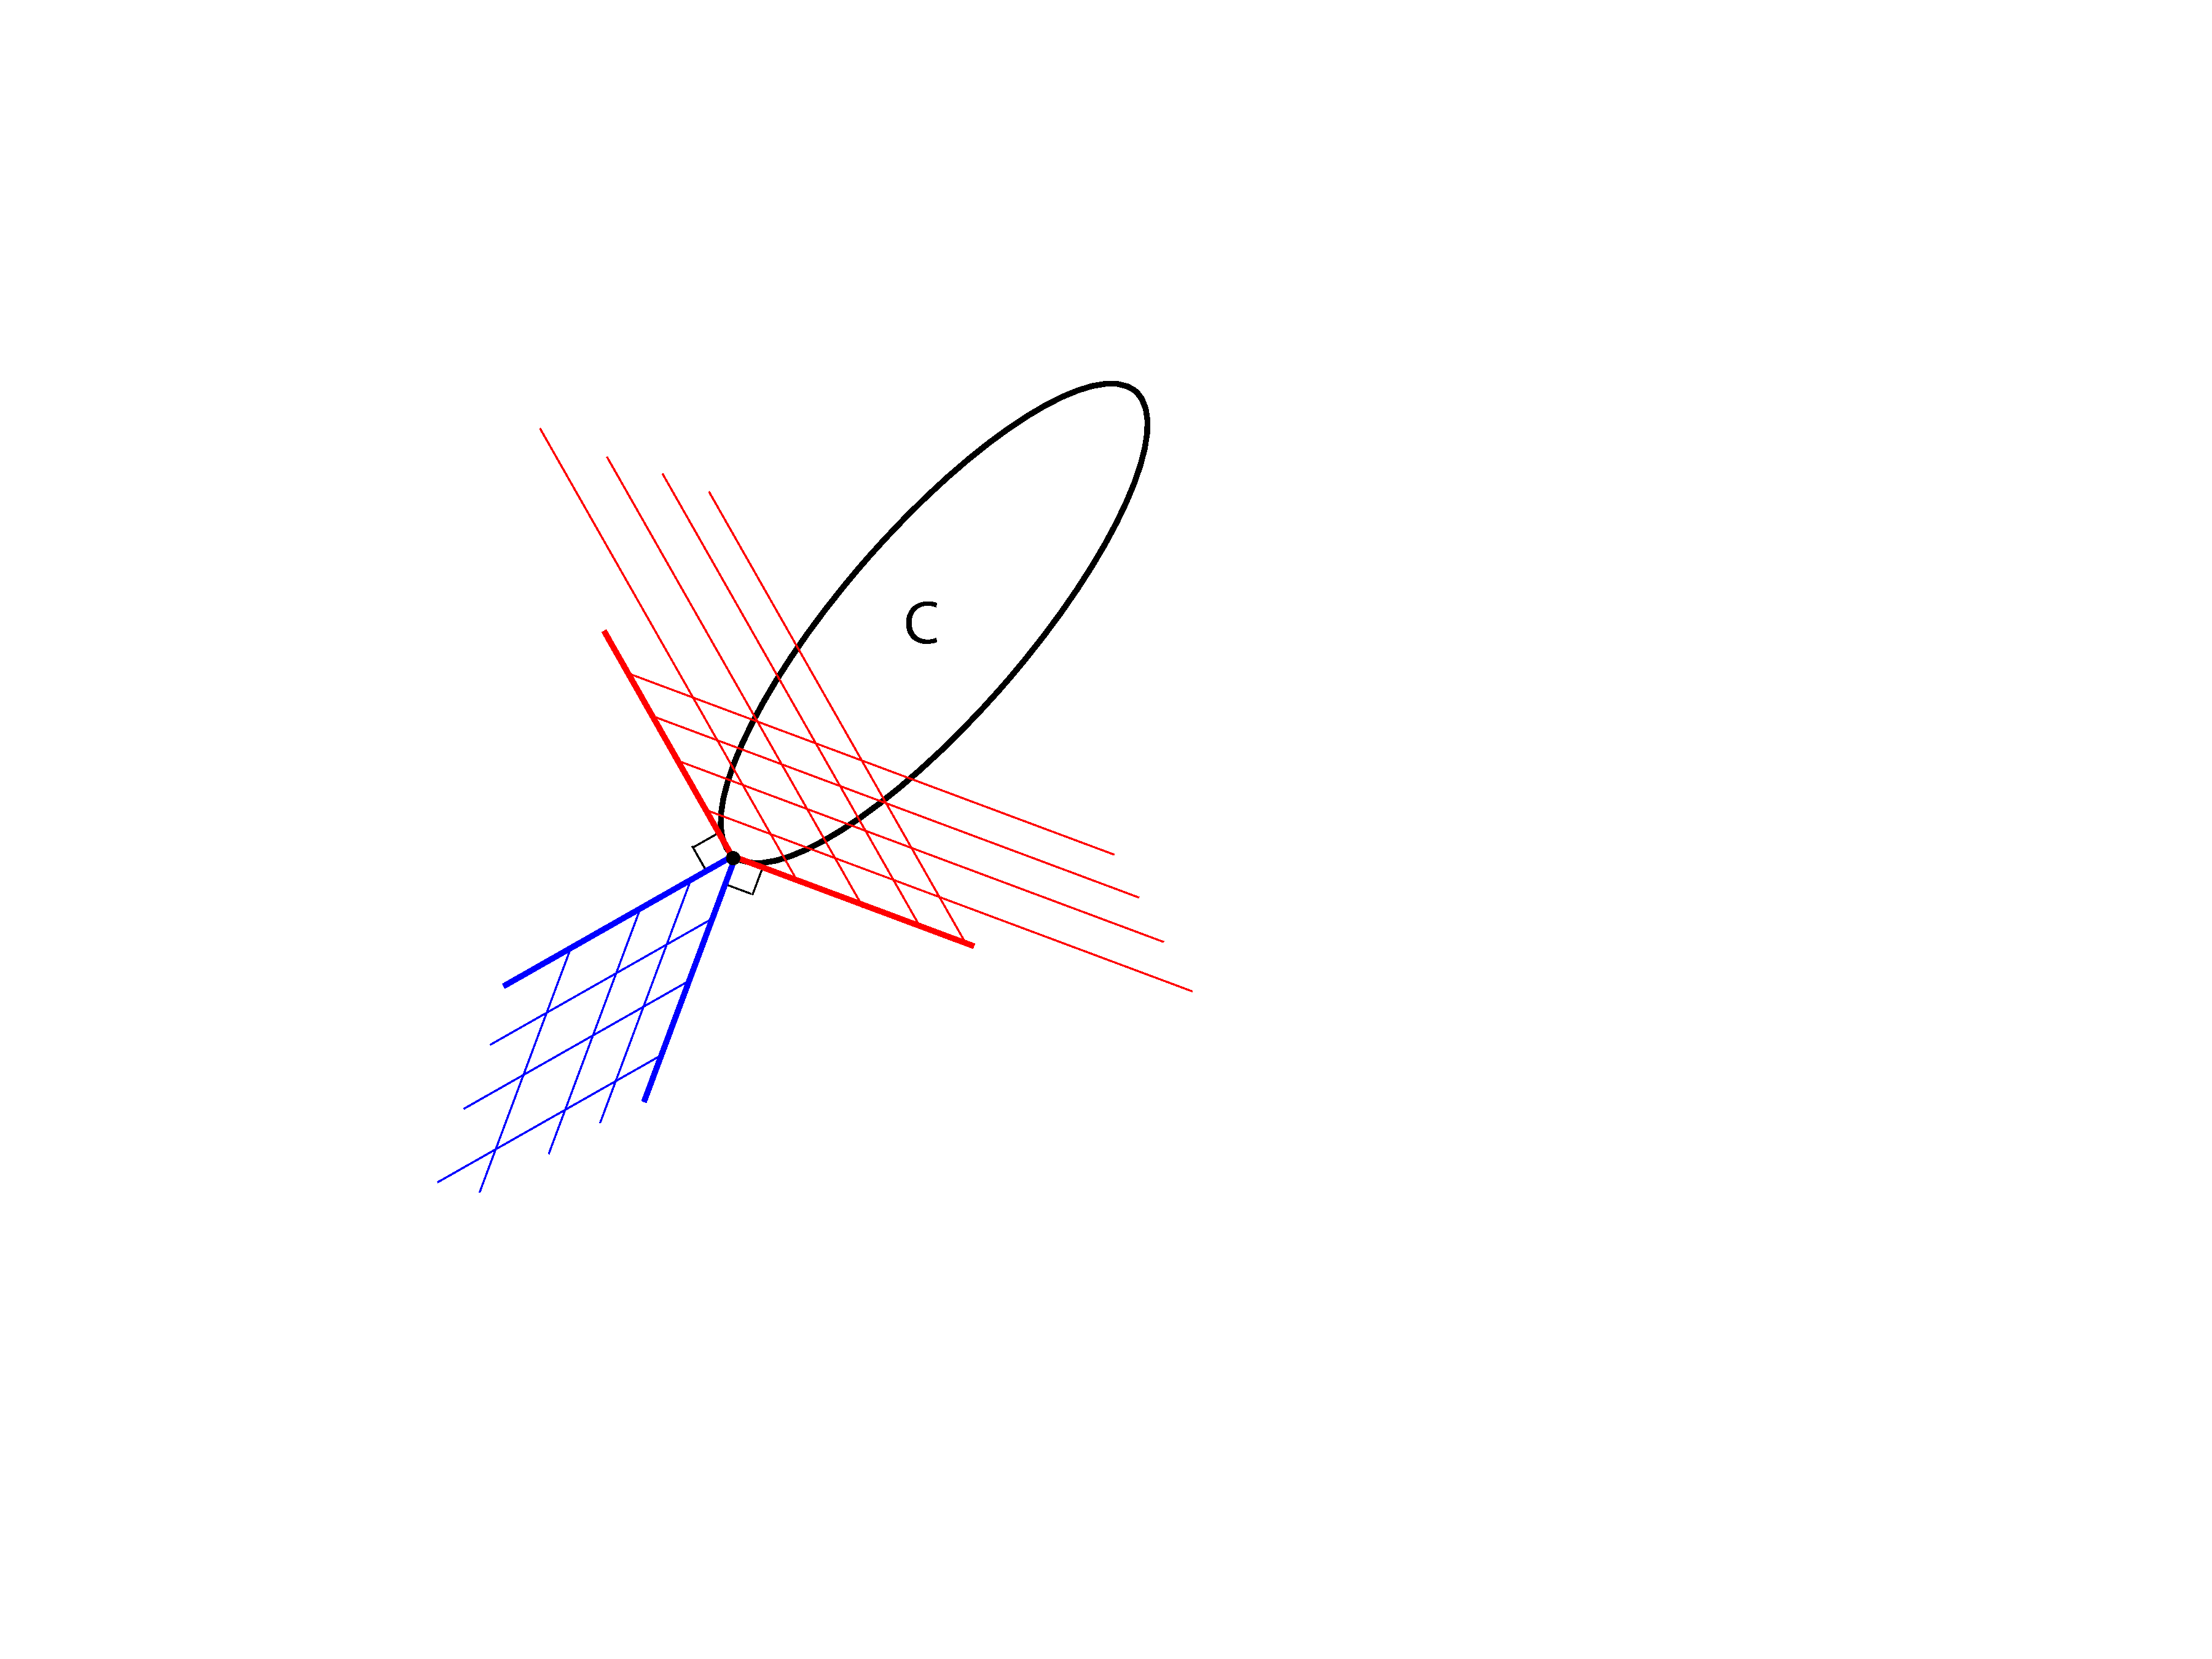
\includegraphics[width=3\textwidth]{figure/lecture13-normal_tangent_cone.pdf} % first figure itself
        % \caption{first figure}
    \end{minipage}\hfill
    \begin{minipage}{0.45\textwidth}
        % \centering
        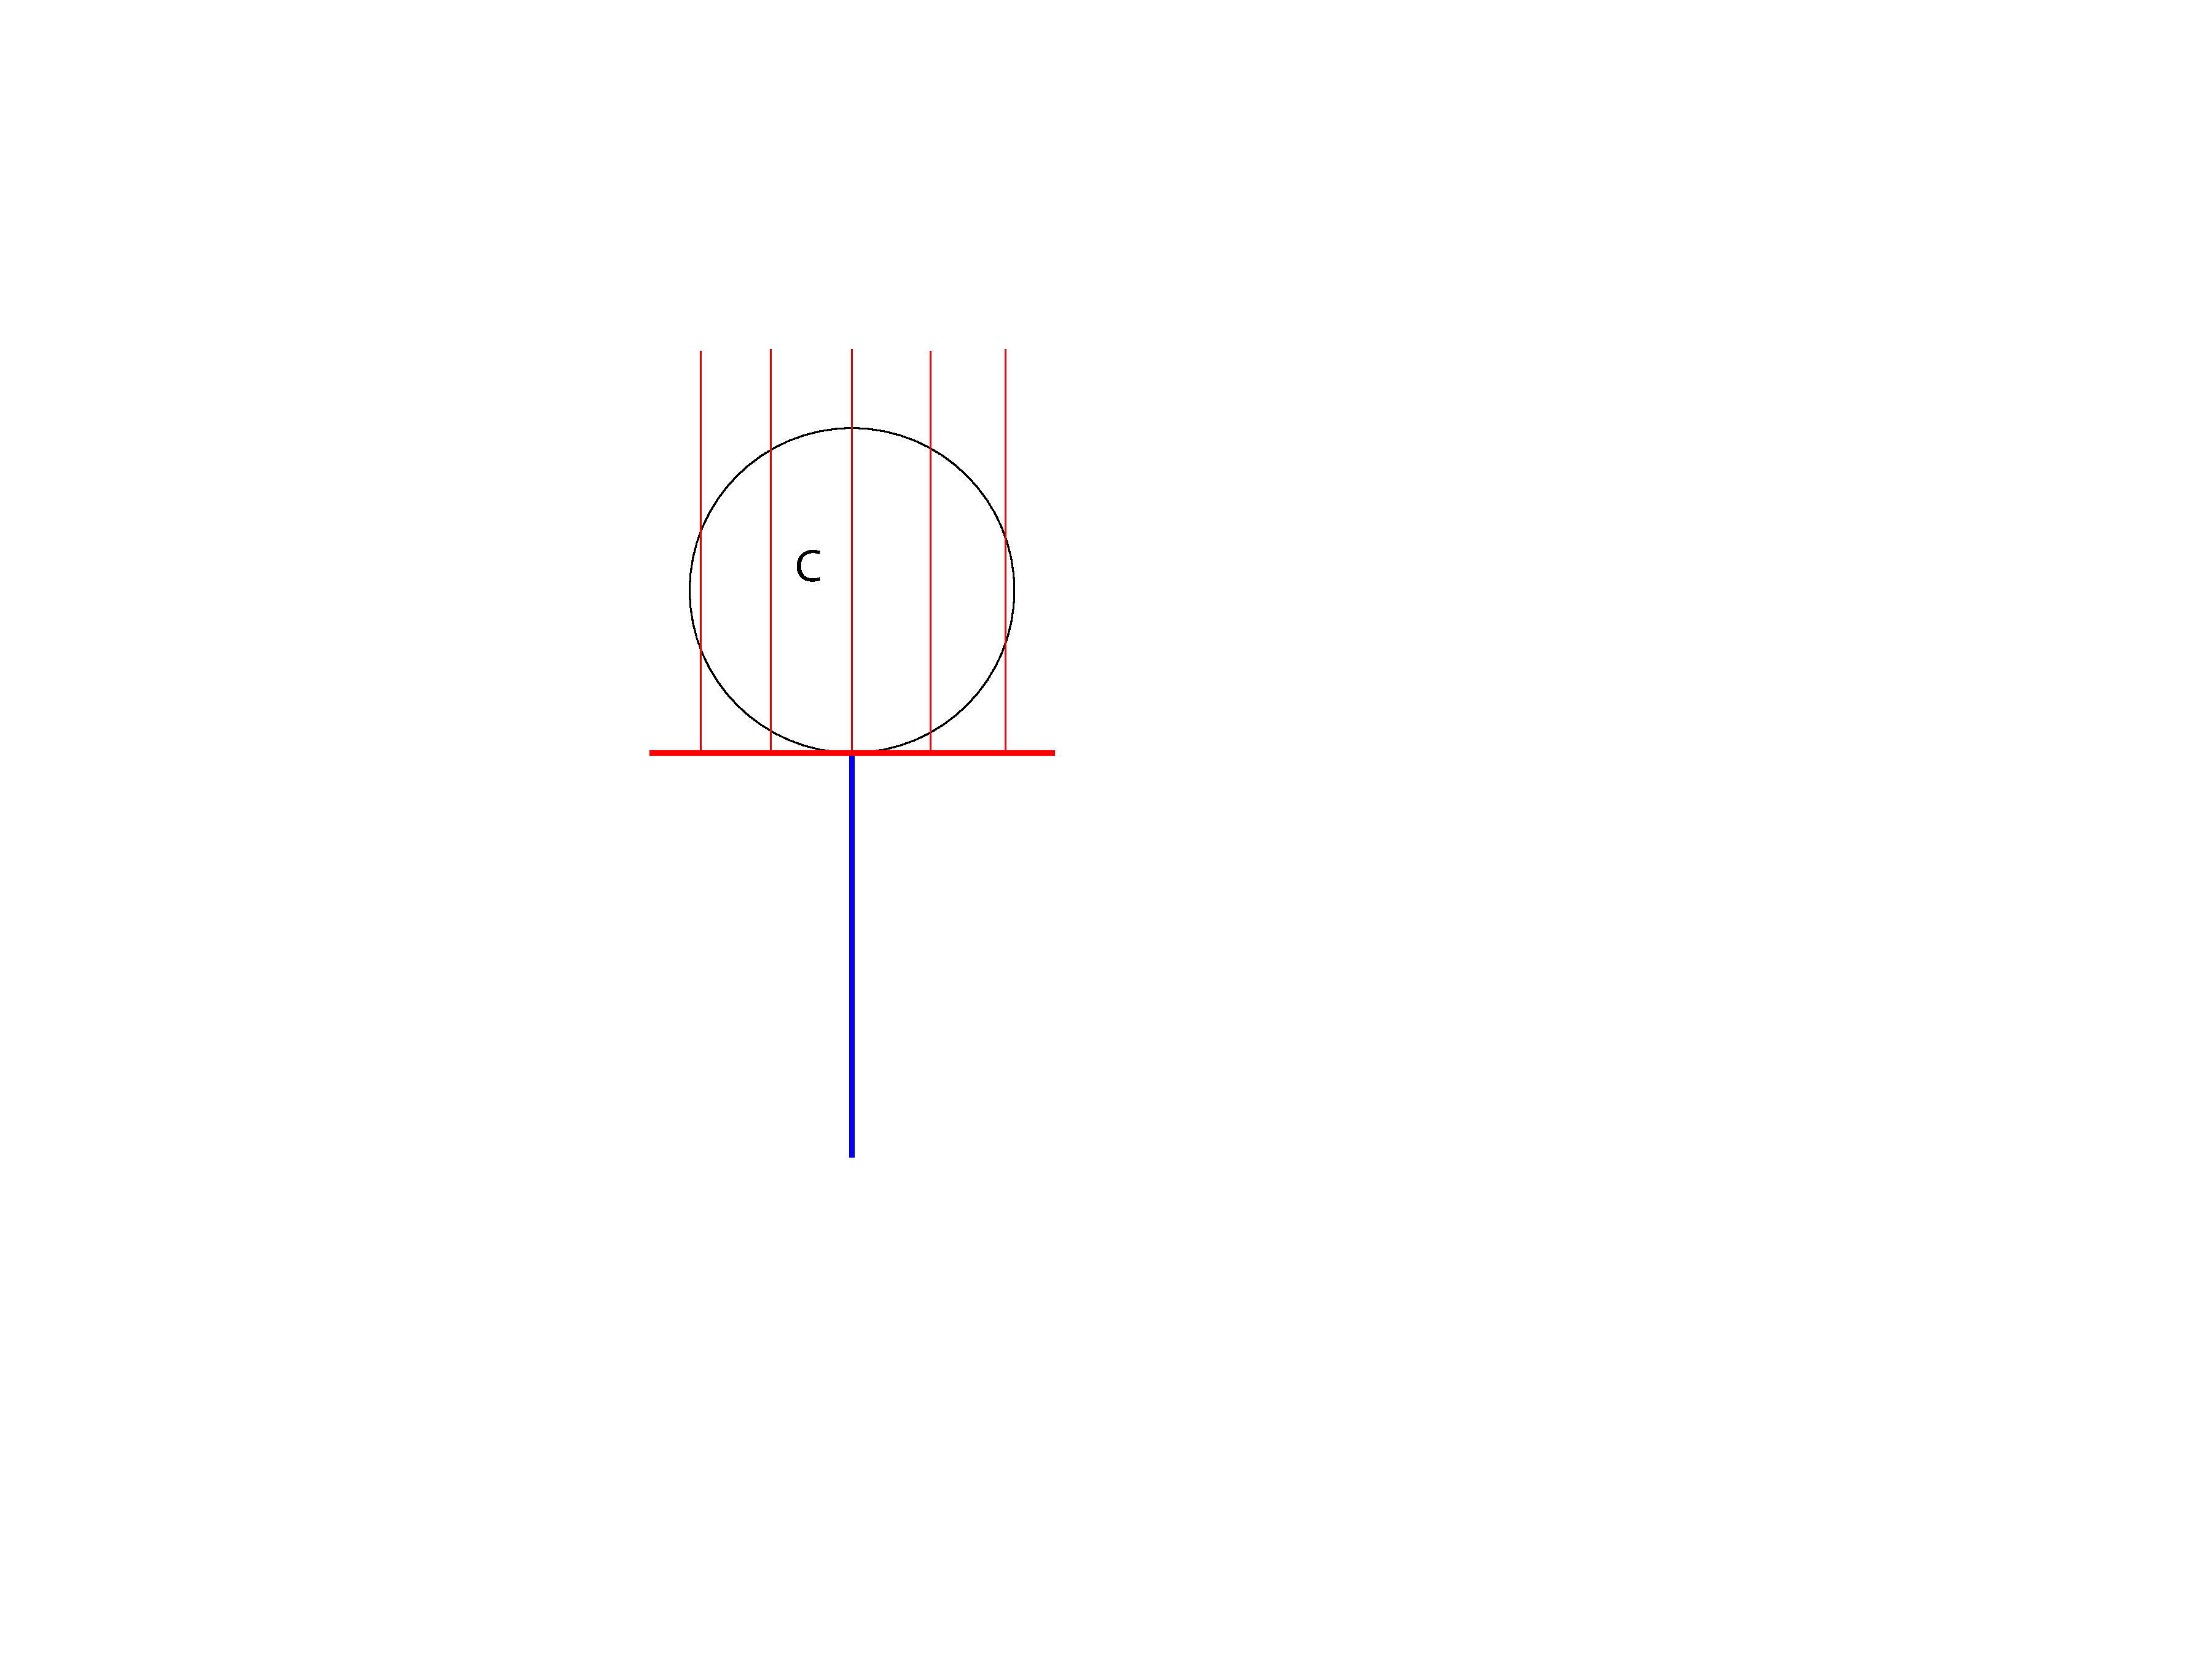
\includegraphics[width=3\textwidth]{figure/lecture13-normal_tangent2.pdf} % second figure itself
        % \caption{second figure}
    \end{minipage}
    \hspace{5cm}
    \vspace{-5cm}
    \caption{Black set is C, red set is $T_C(x)$, blue set is $N_c(x)$}
\end{figure}


% \begin{figure}
% \centering
% \begin{subfigure}{.5\textwidth}
%   \centering
%   \includegraphics[width=8cm]{normal_tangent_cone.pdf}
%   \caption{A subfigure}
%   \label{fig:sub1}
% \end{subfigure}%
% \begin{subfigure}{.5\textwidth}
%   \centering
%   \includegraphics[width=8cm]{normal_tangent2.pdf}
%   \caption{A subfigure}
%   \label{fig:sub2}
% \end{subfigure}
% \caption{A figure with two subfigures}
% \label{fig:test}
% \end{figure}


Suppose we want to minimize a continuously differentiable function $f$ over the intersection of a closed convex set $\Omega$ and an affine set $\mathcal{A} = \{x: Ax=b\}$\begin{equation} \label{eq:constr-opt-affine}
  \begin{array}{ll}
  \text{minimize} &f(x)\\
  \text{subject to} &x \in \Omega\\
  & Ax=b
  \end{array}
  \end{equation}
where $A$ is again a full rank $n\times d$ matrix.  In this section, we will generalize~\eqref{eq:opt-cond} to show

\begin{proposition}\label{prop:constr-opt-affine} $x_\star$ is optimal for~\eqref{eq:constr-opt-affine} if and only if there exists $\lambda_\star \in \R^n$ such that
\[
 \begin{cases}
 - \nabla [f(x_\star) + A^{\trans} \lambda_\star] \in \mathcal{N}_{\Omega} (x_\star)\\
  x_\star \in \Omega \cap \mathcal{A}
  \end{cases}\,.
 \]
\end{proposition}
The key to our analysis here will be to rely on convex analytic arguments. Note that when there is no equality constraint $Ax = b$, our constrained optimality condition is completely equivalent to the assertion
\begin{equation}\label{eq:opt-cond-basic}
  - \nabla f(x_\star) \in \mathcal{N}_{\Omega}(x_\star)\,.
 \end{equation}
Thus, to prove Proposition~\ref{prop:constr-opt-affine}, it will suffice for us to understand the normal cone of the set $\Omega \cap \mathcal{A}$
at the point $x_\star$. To obtain a reasonable characterization, we begin by proving a general fact.
 
\begin{proposition}\label{prop:normal-cone-intersection}
Let $\Omega \subseteq \R^d$ be a closed convex set.  Let $\mathcal{A}$ denote the affine set $\{x~:~Ax = b\}$ for some $A \in \R^{n \times d}$ and $b \in \R^n$.  Suppose that the set $\operatorname{ri}(\Omega) \cap \mathcal{A}$ is non-empty. Then for any $x \in \Omega \cap \mathcal{A}$,
$$\mathcal{N}_{\Omega \cap \mathcal{A}} (x)= \mathcal{N}_{\Omega}(x) + \{A^T \lambda~:~\lambda \in \R^n\}\,.$$
\end{proposition}

\begin{proof}
The ``$\supseteq$'' assertion is straightforward.  To see this, suppose $z \in \Omega \cap \mathcal{A}$ and note that $z-x \in \operatorname{null}(A)$ so that $(z-x)^\trans A^\trans \lambda = \lambda^\trans A(z-x) = 0$ for all $\lambda \in \R^n$. If $u \in \mathcal{N}_{\Omega}(x)$, then $(z-x)^\trans u \le 0$, so for $\lambda\in \R^n$, we have
\[
	\langle z-x, u + A^\trans \lambda \rangle = \langle z-x,u \rangle \leq 0
\]
implying that $u+A^\trans \lambda \in \mathcal{N}_{\Omega \cap \mathcal{A}}(x)$. For the reverse inclusion, let $v \in \mathcal{N}_{\Omega \cap \mathcal{A}}(x)$.  Then we have
\[
	v^\trans (z-x) \leq 0 \text{ for all $z \in \Omega \cap \mathcal{A}$}
\]
Now define the sets
\[
\begin{aligned}
	C_1 &=\left\{ (y,\mu) \in \R^{d+1}~:~ y =z-x,\,\, z\in \Omega,\,\,\mu \leq v^\trans y\right\}\\
	C_2 &= \left\{ (y,\mu) \in \R^{d+1}~:~ y \in \operatorname{ker}(A),\,\,\mu = 0\right\}\,.
\end{aligned}
\]
Note that $\operatorname{ri}(C_1) \cap C_2 = \emptyset$ because otherwise there would exist a $(\hat{y},\hat{\mu})$ such that
\[
	v^\trans \hat{y} > \hat{\mu} = 0
\]
and $\hat{y} \in \mathcal{T}_{\Omega \cap \mathcal{A}}(x)$.  This would contradict our assumption that
$v \in \mathcal{N}_{\Omega \cap \mathcal{A}}(x)$.  Since their intersection is empty, we can properly separate $\operatorname{ri}(C_1)$ from $C_2$.  Indeed, since $C_2$ is a subspace and $C_1$ has nonempty relative interior, there must be a $(w,\gamma)$ such that
\[
	\inf_{(y,\mu)\in C_1} \{ w^\trans y + \gamma \mu\} <	\sup_{(y,\mu)\in C_1} \{ w^\trans y + \gamma \mu\} \leq 0
\]
while
\[
	w^\trans u = 0 \text{ for all $u \in \ker(A)$.}
\]
In particular, this means that $w=A^T \lambda$  for some $\lambda \in \R^n$. Now, $\gamma$ must be nonnegative, as otherwise, 
\[
	\sup_{(y,\mu)\in C_1} \{ w^\trans y + \gamma \mu\} = \infty
\]
(which can be seen by letting $\mu$ tend to negative infinity).  If $\gamma=0$, then
\[
	\sup_{y \in C_1} w^\trans y \leq 0
\]
but the set $\{y~:~w^T y = 0\}$ does not contain the set $\{z-x~:~z\in\Omega\}$ as the infimum is strictly negative.  This means that the relative interior of $\Omega -\{x\}$ cannot intersect the kernel of $A$ which contradicts our assumptions.  Thus, we can conclude that $\gamma$ is strictly positive.  By homogeneity, we may as well assume that $\gamma = 1$.

To complete the argument, note that we now have
\[
 	 (w+v)^\trans (z-x)  \leq 0 \text{ for all $z \in \Omega$.}
\]
This means that $v+w \in \mathcal{N}_{\Omega}(x)$ and we have already shown that $w = A^T\lambda$. Thus, 
\[
v = (v+w)-w \in \mathcal{N}_{\Omega}(x) + \mathcal{N}_{\mathcal{A}}(x)\,.
\]
\end{proof}



Let's now translate the consequence of this proposition for our problem.  Using~\eqref{eq:opt-cond-basic} and Proposition~\ref{prop:normal-cone-intersection}, we have that $x_\star$ is optimal for 
 $$ \min f(x)\;\;\; s.t \;\;\; x \in \Omega, \;\; Ax = b$$ 
 if and only if  $Ax_\star = b$ and there exists a $\lambda \in \R^n$ such that 
 $$ - \nabla [f(x_*) + A^\trans \lambda] \in \mathcal{N}_{\Omega} (x_\star) \;\;\;\; \forall x \in \Omega\,.$$
 This reduction is not immediately useful to us, as it doesn't provide an algorithmic approach to solving the constrained optimization problem.  However, it will form the basis of our dive into duality.
 
 
\subsection{Duality}
 
 Duality lets us associate to any constrained optimization problem, a concave maximization problem whose solutions lower bound the optimal value of the original problem.  In particular, under mild assumptions, we will show that one can solve the primal problem by first solving the dual problem.  
 
We'll continue to focus on the standard primal problem for an equality constrained optimization problem:
  \begin{equation}\label{eq:std-opt}
  \begin{array}{ll}
  \text{minimize} & f(x) \\
  \text{subject to} & x\in\Omega\\
  &Ax = b
    \end{array}
  \end{equation}
 Here, assume that $\Omega$ is a closed convex set, $f$ is differentiable, and $A$ is full rank.
 
 The key behind duality (here, Lagrangian duality) is that problem~\eqref{eq:std-opt} is equivalent to
\[
\min_{x \in \Omega} \max_{\lambda \in \R^n} f(x) + \lambda^T(Ax-b)
\]
To see this, just note that if $Ax\neq b$, then the max with respect to $\lambda$ is infinite.  On the other hand, if $Ax=b$ is feasible, then the max with respect to $\lambda$ is equal to $f(x)$.
 
 The \emph{dual problem} associated with~\eqref{eq:std-opt} is
 \[
 \max_{\lambda \in \R^n} \min_{x \in \Omega} f(x) + \lambda^T(Ax-b)
\]

Note that the function
\[
	q(\lambda): =  \min_{x \in \Omega} f(x) + \lambda^T(Ax-b)
\]
is always a concave function as it is a minimum of linear functions.  Hence the dual problem is a concave maximization problem, regardless of what form $f$ and $\Omega$ take.  We now show that it always lower bounds the primal problem. 

\subsection{Weak Duality}
  
\begin{proposition}
For any function $\varphi(x,z)$,
\[
 \min_x \max_z \varphi(x,z) \geq \max_z \min_x \varphi(x,z)\,.
 \]
\end{proposition}
\begin{proof}
The proof is essentially tautological.  Note that we always have
\begin{align*}
\varphi(x,z) &\geq \min_x \varphi(x,z)
\end{align*}
Taking the maximization with respect to the second argument verifies that
\begin{align*}
\max_z \varphi(x,z) &\geq \max_z \min_x \varphi(x,z) \quad \forall x\,.
\end{align*}
Now, minimizing the left hand side with respect to $x$ proves
\begin{align*}
\min_x \max_z\varphi(x,z) &\geq \max_z \min_x \varphi(x,z)
\end{align*}
which is precisely our assertion.
\end{proof}

\subsection{Strong duality}

For convex optimization problems, we can prove a considerably stronger result.  Namely, that the primal and dual problems attain the same optimal value.  And, moreover, that if we know a dual optimal solution, we can extract a primal optimal solution from a simpler optimization problem.

\begin{theorem}[Strong Duality]\quad\\
\begin{enumerate}
\item If $\exists z \in \operatorname{rel int} (\Omega) $ that also satisfies our equality constraint,  and the primal problem has an optimal solution, then the dual has an optimal solution and the primal and dual values are equal
\item In order for $x_\star$ to be optimal for the primal and $\lambda_\star$ optimal for the dual, it is necessary and sufficient that $Ax_\star = b$ , $x_\star \in \Omega$ and $$x_\star \in \arg\min_{x\in \Omega}\;\; \mathcal{L} (x , \lambda_\star) = f(x) + {\lambda_\star}^T (Ax - b)$$
\end{enumerate}
\end{theorem}
\begin{proof}
For all $\lambda$ and all feasible $x$
\begin{align*}
q(\lambda)&\leq  f(x) + \lambda(Ax -b)= f(x)
\end{align*}
where the second equality holds because $Ax=b$.

Now by Proposition~\ref{prop:constr-opt-affine}, $x_\star$ is optimal if and only if there exists a $\lambda_\star$ such that
\[
 \langle \nabla f(x_\star) + A^T \lambda_\star, x- x_\star \rangle \geq 0~~\forall x\in \Omega\\
 \]
and $Ax_\star=b$.  Note that this condition means that $x_\star$ minimizes $\mathcal{L}(x,\lambda_\star)$ over $\Omega$.

  By preceding argument, it now follows that
  \begin{align*} 
  q(\lambda_\star) &= \inf_{x \in \Omega} \mathcal{L}(x, \lambda_\star)\\
  &= \mathcal{L}(x_\star, \lambda_\star)\\
  & = f(x_\star) + {\lambda_\star}^T(Ax_\star - b) = f(x_\star)
  \end{align*}
  which completes the proof.
\end{proof}  


 \end{document}  

  
  Suppose we want to minimize a smooth function over an intersection of sets \begin{equation*} 
  \begin{array}{ll}
  \text{minimize} &f(x)\\
  \text{subject to} &x \in \Omega_1 \cap \Omega_2 \cap \dots \cap \Omega_k
  \end{array}\,.
  \end{equation*}
 We can rewrite this optimization problem to decouple the constraints as
   \begin{equation*} 
  \begin{aligned} 
  &\text{minimize} &&f(x)\\
  &\text{subject to} &&x_i \in \Omega_i, \;\; x_i = x_j \;\;\;\forall i,j
  \end{aligned}
  \end{equation*}
 This is completely equivalent to the original formulation. 
   
 
 
 


 
 
  \begin{proposition}
 $$ \mathcal{N}_{\Omega_1 \cap \Omega_2}(x) \supseteq \mathcal{N}_{\Omega_1}(x) + \mathcal{N}_{\Omega_2}(x)  $$
 with equality if there is  a point in the intersection of the relative interior of $\Omega_1$
  \end{proposition}
\begin{proof} 
\begin{align*}
\langle v, z - x \rangle \geq 0 \;\;\; \forall z \in \Omega_1\\
\langle v, z - x \rangle \geq 0 \;\;\; \forall z \in \Omega_1 \cap \Omega_2
\end{align*}
same with the roles swapped. Also clearly true for sums.\\
\underline{Conversely}, \\
Suppose $\langle v, z-x \rangle  \geq 0$ but $v \not \in  \Omega_1 \cap \Omega_2$\\
$\exists y$ such that $$\langle v,y \rangle > \langle u_1 + u_2, y \rangle \;\; \forall  u_1 \in \mathcal{N}_{\Omega_1}(x), u_2 \in \mathcal{N}_{\Omega_2}(x)$$
strict separation holds because $\mathcal{N}_{\Omega_1}$ is closed and $\mathcal{N}_{\Omega_2}$ is affine (see Bertsekas)\\
\end{proof}

\section{Lecture 14: Algorithms using Duality}

The Lagrangian duality theory from the previous lecture can be used to
design improved optimization algorithms which perform the optimization
on the dual function. Oftentimes, passing to the dual can simplify
computation or enable parallelization.

\subsection{Review}

Recall the \emph{primal problem}
\[
\min_{x \in \Omega} f(x) : A x = b
\]
The corresponding dual problem is obtained by considering the
\emph{Lagrangian}
\[
L(x,\lambda) = f(x) + \lambda^T(A x  - b)
\]
where $\lambda_i$ are called \emph{Lagrange multipliers}. The
\emph{dual function} is defined as
\[
g(\lambda) = \inf_{x \in \Omega} L(x,\lambda)
\]
and the \emph{dual problem} is
\[
\sup_{\lambda \in \R^m} g(\lambda)
\]

\begin{definition}[Concave functions]
$f$ is concave $\iff -f$ is convex.
\end{definition}

\begin{fact}
The dual function is always concave (even if $f$ and
$\Omega$ are not convex).
\end{fact}

\begin{proof}
For any $x \in \Omega$,
$L(x,\lambda)$ is a linear function of $\lambda$ so $g(\lambda)$
is an infimum over a family of linear functions, hence concave.
\end{proof}

\subsection{Dual gradient ascent}

Concavity of the dual function $g(\lambda)$ ensures existence of
subgradients, so the subgradient method can be applied to optimize $g(\lambda)$.
The \emph{dual gradient ascent} algorithm is as follows:

Start from initial $\lambda_0$.
For all $t \geq 0$:
\[
x_t = \arg\inf_{x \in \Omega} L(x, \lambda_t)
\]
\[
\lambda_{t+1} = \lambda_t + \eta (A x_t - b)
\]

This yields the $O(1/\sqrt{t})$ convergence rate obtained by the
subgradient method.

\subsection{Augmented Lagrangian method / method of multipliers}

Whereas dual gradient ascent updates $\lambda_{t+1}$ by taking a step
in a (sub)gradient direction, a method known as the \emph{dual proximal
method} can be motivated by starting with using the proximal operator \cite{parikh2014proximal}
as an update rule for iteratively optimizing $\lambda$:

\[
\lambda_{t+1}
= \mathrm{prox}_{\eta_t g}(\lambda_t)
 = \arg\sup_{\lambda} \underbrace{\underbrace{\inf_{x \in \Omega} f(x) + \lambda^T (A x - b)}_{g(\lambda)} - \underbrace{\frac{1}{2 \eta_t} \|\lambda - \lambda_t\|^2}_{\text{proximal term}}}_{h(\lambda)}
\]

Notice that this expression includes a proximal term which makes
$h(\lambda)$ strongly convex.

However, this update rule is not always directly useful since it requires
optimizing $h(\lambda)$ over $\lambda$, which may not be available
in closed form. Instead, notice that if we can interchange $\inf$ and
$\sup$ (e.g.~strong duality, Sion's theorem applied when $\Omega$ is
compact) then we can rewrite
\begin{align}
\sup_{\lambda} \inf_{x \in \Omega} f(x) + \lambda^T(A x - b) - \frac{1}{2 \eta_t} \|\lambda - \lambda_t\|^2 &= \inf_{x \in \Omega} \sup_\lambda f(x) + \lambda^T(A x - b) - \frac{1}{2\eta_t} \|\lambda_t - \lambda\|^2 \\
&= \inf_{x \in \Omega} f(x) + \lambda_t^T (A x - b) + \frac{\eta_t}{2}\|A x - b\|^2
\end{align}
where the inner $\sup$ is optimized in closed-form by
$\lambda = \lambda_t + \eta_t(A x - b)$. To isolate the remaining
optimization over $x$, we make the following definition.

\begin{definition}[Augmented Lagrangian]
The \emph{augmented Lagrangian} is
\[L_\eta(x,\lambda) = f(x) + \lambda_t^T (A x - b) + \frac{\eta_t}{2}\|A x - b\|^2\]
\end{definition}

The \emph{augmented Lagrangian method} (aka Method of Multipliers) is
defined by the following iterations:
\[
x_t = \arg\inf_{x \in \Omega} L_{\eta_t} (x, \lambda_t)
\]
\[
\lambda_{t+1} = \lambda_t + \eta_t (A x_t - b)
\]

While the iterations look similar to dual gradient ascent, there are
some noteworthy differences
\begin{itemize}
\item The method of multipliers can speed up
convergence (e.g.~for non-smooth functions), but computing $x_t$ may
be more difficult due to the additional
$\frac{\eta_t}{2} \|A x - b\|^2$ term in the augmented Lagrangian
\item $L(x, \lambda_t)$ is convex in $x$, but $L_\eta(x, \lambda_t)$ is
strongly convex in $\lambda$ (if $A$ is full-rank)
\item Convergence at
a $O(1/t)$ rate. More precisely, for constant step size $\eta$, we
can show show the method of multipliers satisfies
\[g(\lambda_t) - g^* \geq -\frac{\|\lambda^*\|^2}{2\eta t}\]
\end{itemize}

\subsection{Dual decomposition}

A major advantage of dual decomposition that it can lead to update rules
which are trivially parallelizable.

Suppose we can partition the primal problem into blocks of size
$(n_i)_{i=1}^N$, i.e.
\begin{align}
x ^T = ((x^{(1)})^T, \cdots, (x^{(N)})^T) &\qquad& x_i \in \R^{n_i}, \sum_{i=1}^N n_i = n \\
A = [A_1 \vert \cdots \vert A_N] &\qquad& A x = \sum_{i=1}^N A_i x^{(i)} \\
f(x) = \sum_{i=1}^N f_i(x^{(i)})
\end{align}

Then the Lagrangian is also separable in $x$
\[
L(x, \lambda) = \sum_{i=1}^N \left( f_i(x^{(i)}) + \lambda^T A_i x^{(i)} - \frac{1}{N} \lambda^T b\right) = \sum_{i=1}^N L_i(x^{(i)}, \lambda)
\]

Each term in the sum consists of one non-interacting partition
$(x^{(i)}, A_i, f_i)$, so minimization of each term in the sum can
occur in parallel. This leads to the \emph{dual decomposition
algorithm}:

\begin{itemize}
\item
  In parallel on worker nodes:
  $x_t^{(i)} = \arg\inf_{x^{(i)}} L_i(x^{(i)}, \lambda_t)$
\item
  On a master node: $\lambda_{t+1} = \lambda_t + \eta (A x - b)$
\end{itemize}

\begin{example}[Consensus optimization]
Consensus optimization is an
application that comes up in distributed computing which can be solved
using dual decomposition. Given a graph $G = (V, E)$,
\[
\min_x \sum_{v \in V} f_v(x_v) : x_v = x_u~\forall(u,v) \in E
\]
This problem is separable over $v \in V$, so dual decomposition applies.

\end{example}

\begin{example}[Network utility maximization]
Suppose we have a
network with $k$ links, each with capacity $c_i$. We are interested
in allocating $N$ different flows with fixed routes over these links such that
utility is maximized and resource constraints are not exceeded.
Let $x_i \in \R^N$ represent the amount of flow $i$ allocated and
$U_i : \R \to \R$ a convex utility function which
returns the amount of utility obtained from having $x_i$ amount of
flow $i$. The optimization problem is
\[
\max_x \sum_{i=1}^N U_i(x_i) : R x \leq c
\]
where $R$ is a $k \times N$ matrix whose $(k,i)$th entry gives the
amount of the capacity of link $k$ is consumed by flow $i$.

To rewrite the primal problem in standard form (i.e.~as a minimization),
take negatives:
\[
\min_x -\sum_i U_i(x^{(i)}) : R x \leq c
\]

The dual problem is then
\[
\max_{\lambda \geq 0} \min_x \sum_i -U_i(x^{(i)}) + \lambda^T (R x - c)
\]
where the $R x \leq c$ primal inequality constraint results in the $\lambda \geq 0$ constraint.
The second term can be rewritten as $\lambda^T\left(\sum_i R_i x_i - \frac{1}{N}c\right)$,
showing that the dual splits over $i$ and hence dual decomposition applies. This leads to a
parallel algorithm which each worker node computes
\[
\arg\max_{x_i} U_i(x_i) - \lambda^T R_i x_i
\]
and the master node computes
\[
\lambda_{t+1} = \left[\lambda_t + \eta (R x - c)\right]_+
\]
We take the positive part because of the $\lambda \geq 0$ constraint.

\textbf{Aside}: In resource allocation problems, the values of the dual variables
$\lambda$ at the optimal point have an economic interpretation as
``prices'' to the resources. In this example, $\lambda_k$ can be
interpreted as the utility per unit of flow over link $k$.
\end{example}

\subsection{ADMM --- Alternating direction method of multipliers}

While dual decomposition can be used to parallelize dual subgradient ascent,
it doesn't work with the augmented Lagrangian. This is because the coupling between
the decision variables introduced by the $\| A x - b \|^2$ term prevents
the augmented Lagrangian from being separable over $x$.

The goal of the alternating direction method of multipliers (ADMM) is to obtain
the best of both worlds: we would like both the parallelism offered by the method
of multipliers as well as the faster convergence rate of the augmented Lagrangian.
We will see that similar to dual decomposition, ADMM partitions
the decision variables into two blocks. Also, similar to the method of multiplers,
ADMM uses the augmented Lagrangian $L_\eta(x,z,\lambda_t)$.

Consider a problem of the form
\[
\min_{x,z} f(x) + g(z) : A x + B z \leq c
\]
In other words, we can split the objective and constraints into two blocks $x$ and $z$.

The method of multipliers would jointly optimize the augmented Lagrangian
on both blocks in one single optimization step:
\begin{align}
(x_{t+1}, z_{t+1}) &= \inf_{x,z} L_\eta(x,z,\lambda_t)\\
\lambda_{t+1} &= \lambda_t + \eta(A x_{t+1} + B z_{t+1} - c)
\end{align}

In contrast, ADMM alternates (the ``A'' in ``ADMM'') between optimizing
the augmented Lagrangian over $x$ and $z$:
\begin{align}
x_{t+1} &= \inf_{x} L_\eta(x, z_t, \lambda_t) \\
z_{t+1} &= \inf_{z} L_\eta(x_{t+1}, z, \lambda_t) \\
\lambda_{t+1} &= \lambda_t + \eta(A x_{t+1} + B z_{t+1} - c)
\end{align}

Unlike the method of multipliers, this is not parallelizable
since $x_{t+1}$ must be computed before $z_{t+1}$. Also, convergence
guarantees are weaker: rather than getting a convergence rate we only get an asymptotic
convergence guarantee.

\begin{theorem}
Assume
\begin{itemize}
\item $f$, $g$ have a closed, non-empty, convex
epigraph
\item $L_0$ has a saddle $x^*$, $z^*$, $\lambda^*$, i.e.:
\[
\forall x,z,\lambda: L_0(x^*,z^*,\lambda) \leq L_0(x^*,z^*,\lambda^*)\leq L(x,z,\lambda^*)
\]
\end{itemize}
Then, as $t \to \infty$, ADMM satisfies
\begin{align}
f(x_t) + g(z_t) &\to p^*\\
\lambda_t &\to \lambda^*
\end{align}
\end{theorem}

\textbf{Aside}: Saddles are useful because $\inf$ and the $\sup$ can
be swapped. To see this, note the saddle condition
\[L(x^*, \lambda) \leq L(x^*, \lambda^*) \leq L(x, \lambda^*)\]
implies that
\begin{align}
\inf_x \sup_\lambda L(x,\lambda)
&\leq \sup_\lambda L(x^*, \lambda)\\
&\leq L(x^*, \lambda^*) \\
&= \inf_x L(x, \lambda^*) \\
&\leq \sup_\lambda \inf_x L(x,\lambda)
\end{align}

\section{Fenchel duality and algorithms}

In this section, we introduce the Fenchel conjugate. First, recall that for a real-valued convex function of a single variable $f(x)$, we call $f^*(p) := \sup_x px - f(x)$ its Legendre transform. This is illustrated in figure \ref{fig:leg-conj}.

\begin{figure}[h]
    \centering
    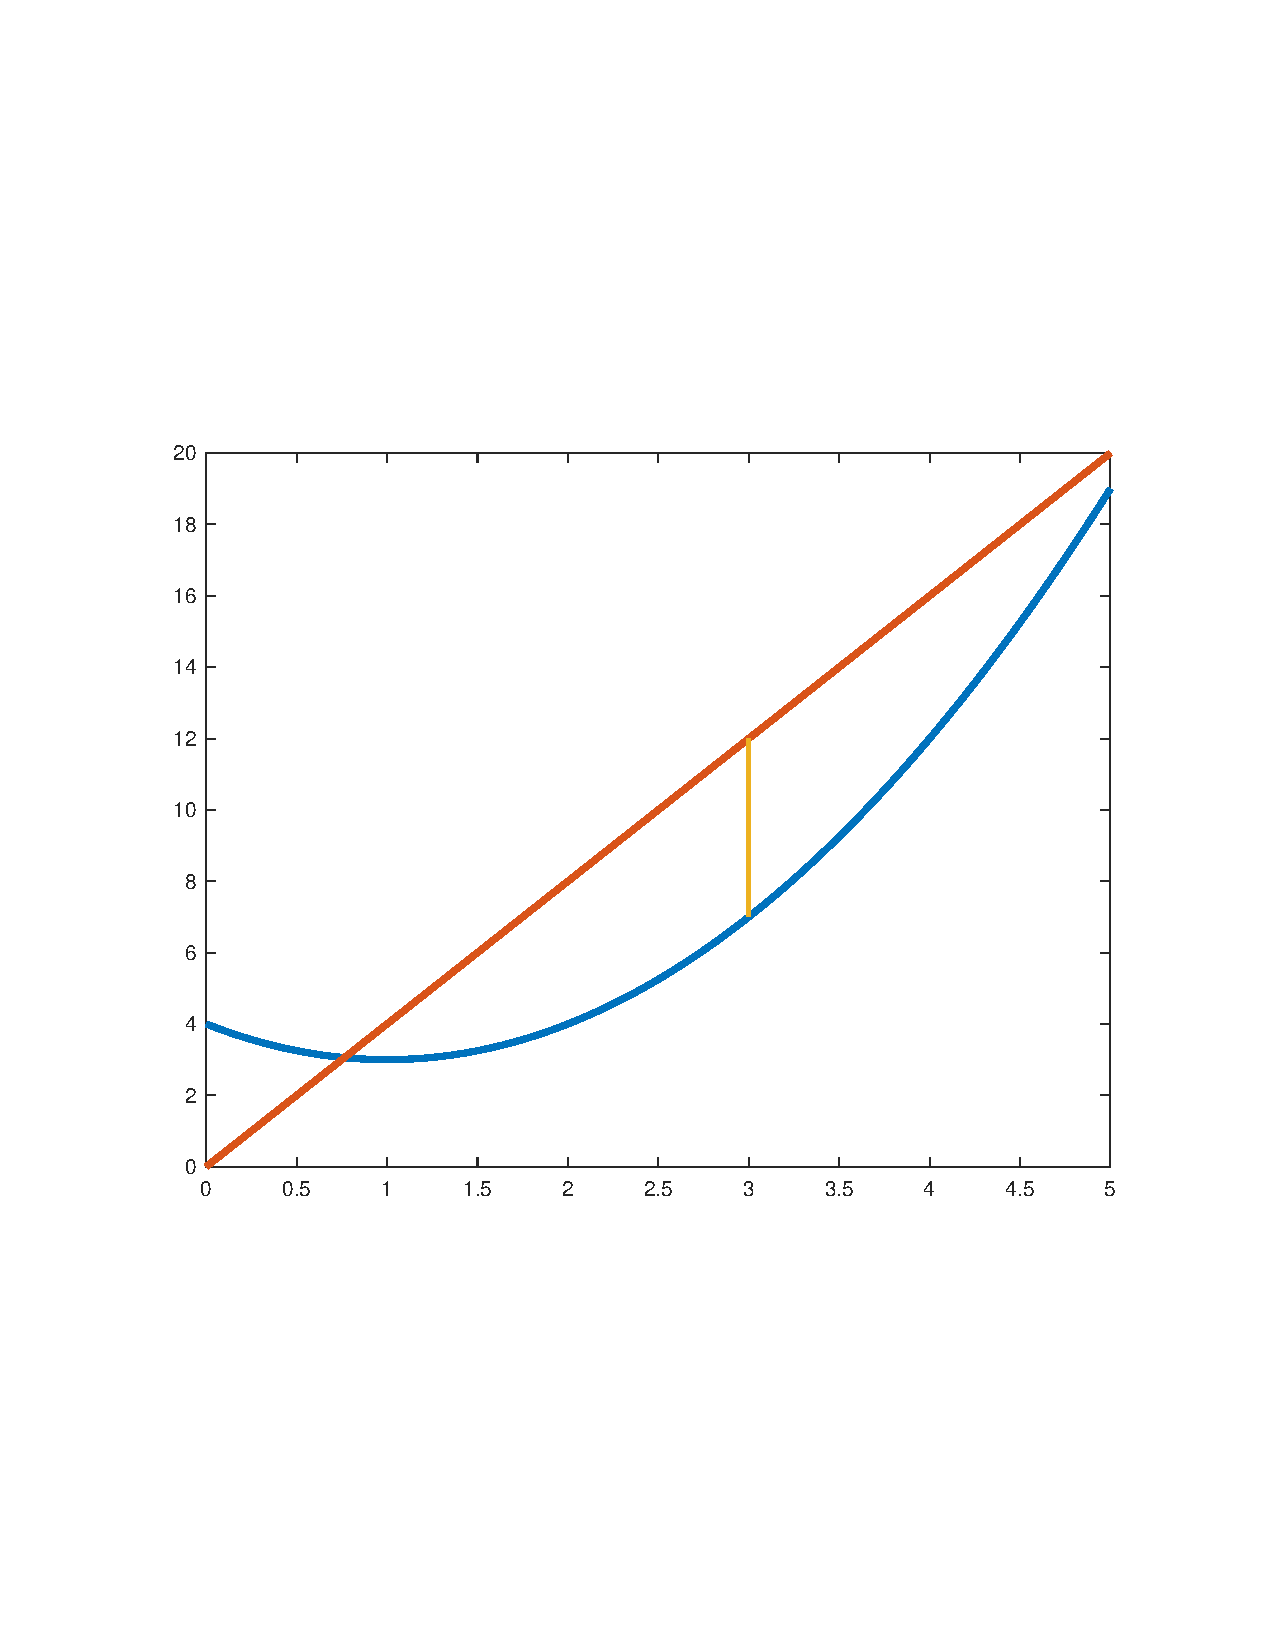
\includegraphics[width=.75\textwidth, trim = 0 200 0 200, clip]{figures/lecture15-conjugate.pdf}
    \caption{Legendre Transform. The function $f^*(p)$ is how much we need to vertically shift the epigraph of $f$ so that the linear function $px$ is tangent to $f$ at $x$.}
    \label{fig:leg-conj}
\end{figure}

The generalization of the Legendre transform to (possibly nonconvex) functions of multiple variables is the Fenchel conjugate.
\begin{definition}[Fenchel conjugate]
The Fenchel conjugate of $f:\R^n \to \R$ is \[f^*(p) = \sup_x \iprod{p,x} - f(x)\]
\end{definition}

We now present several useful facts about the Fenchel conjugate. The proofs are left as an exercise.

\begin{fact}
$f^*$ is convex.
\end{fact}

Indeed, $f^*$ is the supremum of affine functions and therefore convex. Thus, the Fenchel conjugate of $f$ is also known as its convex conjugate.

\begin{fact}
$f^*(f^*(x)) = f$ if $f$ is convex.
\end{fact}

In other words, the Fenchel conjugate is its own inverse for convex functions. Now, we can also relate the subdifferential of a function to that of its Fenchel conjugate. Intuitively, observe that $0 \in \partial f^*(p) \iff 0 \in  p - \partial f(x) \iff p \in \partial f(x)$. This is summarized more generally in the following fact.

\begin{fact}
The subdifferential of $f^*$ at $p$ is $\partial f^*(p) = \{x: p \in \partial f(x)\}$. 
\end{fact}

Indeed, $\partial f^*(0)$ is the set of minimizers of $f$. 

In the following theorem, we introduce Fenchel duality.

\begin{theorem}[Fenchel duality]\label{thm:fenchel}
Suppose we have $f$ proper convex, and $g$ proper concave. Then \[\min_x f(x)- g(x) = \max_p g^*(p) - f^*(p) \]
where $g^*$ is the concave conjugate of $g$, defined as $\inf_x \iprod{p,x} - g(x)$.
\end{theorem}

In the one-dimensional case, we can illustrate Fenchel duality with Figure \ref{fig:fenc_conj}.

	
\begin{figure}[h]
	\centering
		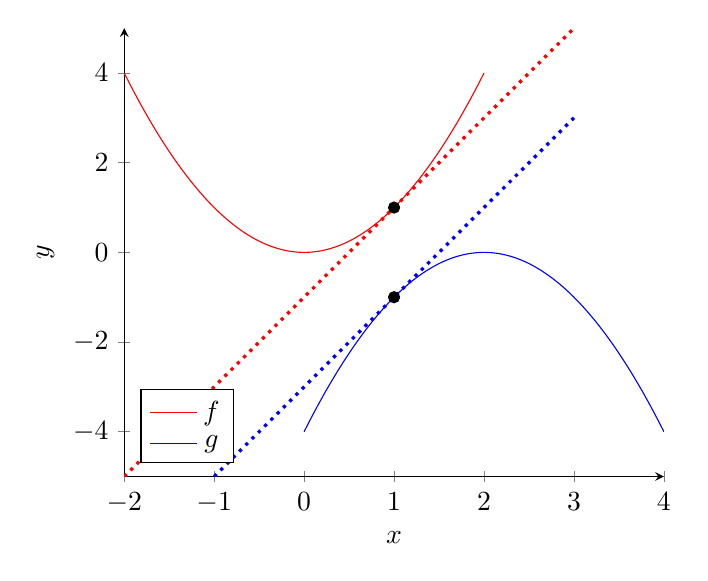
\begin{tikzpicture}
		\begin{axis}[
		axis lines = left,
		xlabel = $x$,
		ylabel = {$y$},
		legend pos=south west,
		]
		%Below the red parabola is defined
		\addplot [
		domain=-2:2, 
		samples=100, 
		color=red,
		]
		{x^2};
		\addlegendentry{$f$}
		%Here the blue parabola is defined
		\addplot [
		domain=0:4, 
		samples=100, 
		color=blue,
		]
		{-1*(x-2)^2};
		\addlegendentry{$g$}
		
		\addplot [
		domain=-1:3, 
		samples=100, 
		color=blue,
		dotted,very thick
		]
		{2*x-3};
		
		\addplot [
		domain=-2:3, 
		samples=100, 
		color=red,
		dotted, very thick
		]
		{2*x-1};
		
		\filldraw[black]  (axis cs:1,1) circle (2pt) ;
		\filldraw[black]  (axis cs:1,-1) circle (2pt);
		
		\end{axis}
		\end{tikzpicture}
		\caption{Fenchel duality in one dimension}\label{fig:fenc_conj}
\end{figure}

In the minimization problem, we want to find $x$ such that the vertical distance between $f$ and $g$ at $x$ is as small as possible. In the (dual) maximization problem, we draw tangents to the graphs of $f$ and $g$ such that the tangent lines have the same slope $p$, and we want to find $p$ such that the vertical distance between the tangent lines is as large as possible. The duality theorem above states that strong duality holds, that is, the two problems have the same solution.

We can recover Fenchel duality from Lagrangian duality, which we have already studied. To do so, we need to introduce a constraint to our minimization problem in Theorem \ref{thm:fenchel}. A natural reformulation of the problem with a constraint is as follows.
\begin{equation}
    \min_{x,z} f(x)-g(z) \text{ subject to } x=z
\end{equation}



\subsection{Deriving the dual problem for empirical risk minimization}
In empirical risk minimization, we often want to minimize a function of the following form:
\begin{equation}
    P(w) = \sum_{i=1}^m \phi_i(\iprod{w,x_i}) + R(w)
\end{equation}

We can think of $w \in \R^n$ as the model parameter that we want to optimize over (in this case it corresponds to picking a hyperplane), and $x_i$ as the features of the $i$-th example in the training set. $\phi_i(\cdot, x_i)$ is the loss function for the $i$-th training example and may depend on its label. $R(w)$ is the regularizer, and we typically choose it to be of the form $R(w) = \frac{\lambda}{2}\norm{w}^2$.

The primal problem, $\min_{w\in \R^n}P(w)$, can be equivalently written as follows:
\begin{equation}
    \min_{w,z}  \sum_{i=1}^m \phi_i(z_i) + R(w) \text{ subject to } X^\top w=z
\end{equation}
By Lagrangian duality, we know that the dual problem is the following:
\begin{align*}
    &\max_{\alpha \in \R^m} \min_{z,w} \sum_{i=1}^m \phi_i(z_i) + R(w) - \alpha^\top(X^\top w-z) \\
    =&\max_\alpha \min_{w,z} \sum_{i=1}^m \phi_i(z_i) + \alpha_iz_i + R(w) - \alpha^\top X^\top w \\
    =&\max_\alpha \left(- \min_{w,z} - \left(\sum_{i=1}^m \phi_i(z_i)  + \alpha_iz_i \right) + (X\alpha)^\top w -R(w) \right) \\
    =& \max_\alpha - \left( \sum_{i=1}^m \max_{z_i} \left( - \phi_i(z_i) - \alpha_iz_i \right) + \max_w (X\alpha)^\top w - R(w)    \right) \\
    =& \max_\alpha -\sum_{i=1}^n \phi_i^*(-\alpha_i) -R^*(X\alpha)
\end{align*}
where $\phi_i^*$ and $R^*$ are the Fenchel conjugates of $\phi_i$ and $R^*$ respectively.
Let us denote the dual objective as $D(\alpha) = \sum_{i=1}^m \phi_i^*(-\alpha_i) - R^*(X\alpha)$. By weak duality, $D(\alpha) \leq P(w)$.

For $R(w) = \frac{\lambda}{2}\norm{w}^2$, $R^*(p) = \frac{\lambda}{2} \norm{\frac{1}{\lambda} p}^2$. So $R$ is its own convex conjugate (up to correction by a constant factor). In this case the dual becomes:
\[\max_\alpha \sum_{i=1}^m \phi_i^*(-\alpha_i) - \frac{\lambda}{2} \norm{\frac{1}{\lambda} \sum_{i=1}^m \alpha_ix_i}^2 \]

We can relate the primal and dual variables by the map $w(\alpha) = \frac{1}{\lambda} \sum_{i=1}^m \alpha_ix_i$. In particular, this shows that the optimal hyperplane is in the span of the data. Here are some examples of models we can use under this framework.

\begin{example}[Linear SVM]
We would use the hinge loss for $\phi_i$. This corresponds to \[\phi_i(w) = \max(0,1-y_ix_i^\top w)~,\quad -\phi_i^*(-\alpha_i) = \alpha_i y_i\]
\end{example}

\begin{example}[Least-squares linear regression]
We would use the squared loss for $\phi_i$. This corresponds to \[\phi_i(w) = (w^\top x_i-y_i)^2~,\quad -\phi_i^*(-\alpha_i) = \alpha_i y_i + \alpha^2/4\]
\end{example}

We end with a fact that relates the smoothness of $\phi_i$ to the strong convexity of $\phi_i^*$.

\begin{fact}
If $\phi_i$ is $\frac{1}{\gamma}$-smooth, then $\phi^*_i$ is $\gamma$-strongly convex.
\end{fact}

\subsection{Stochastic dual coordinate ascent (SDCA)}

In this section we discuss a particular algorithm for empirical risk minimization which makes use of Fenchel duality. Its main idea is picking an index $i\in[m]$ at random, and then solving the dual problem at coordinate $i$, while keeping the other coordinates fixed.

More precisely, the algorithm performs the following steps:
\begin{enumerate}
\item Start from $w^0:=w(\alpha^0)$
\item For $t=1,\dots, T$:
    \begin{enumerate}
        \item Randomly pick $i\in[m]$
        \item Find $\Delta\alpha_i$ which maximizes
        $$-\Phi_i\left(-(\alpha_i^{t-1}+\Delta\alpha_i)\right)-\frac{\lambda}{2m}\Norm{w^{t-1}+\frac{1}{\lambda}\Delta\alpha_ix_i}^2$$
    \end{enumerate}
\item Update the dual and primal solution
    \begin{enumerate}
        \item $\alpha^t = \alpha^{t-1}+\Delta\alpha_i$
        \item $w^t = w^{t-1} + \frac{1}{\lambda} \Delta\alpha_ix_i$
    \end{enumerate}
\end{enumerate}
For certain loss functions, the maximizer $\Delta\alpha_i$ is given in closed form. For example, for hinge loss it is given explicitly by:
$$\Delta\alpha_i = y_i\max\left(0,\min(1,\frac{1-x_i^Tw^{t-1}y_i}{\|x_i\|^2/\lambda m} + \alpha_i^{t-1}y_i)\right) - \alpha_i^{t-1},$$
and for squared loss it is given by:
$$\Delta\alpha_i = \frac{y_i - x_i^Tw^{t-1} - 0.5\alpha_i^{t-1}}{0.5 + \|x\|^2/\lambda m}.$$
Note that these updates require both the primal and dual solutions to perform the update.

Now we state a lemma given in $\cite{shalev2013}$, which implies linear convergence of SDCA. In what follows, assume that $\|x_i\|\leq 1$, $\Phi_i(x)\geq 0$ for all $x$, and $\Phi_i(0)\leq 1$.

\begin{lemma}
\lemmalabel{sdcaconv}
Assume $\Phi_i^*$ is $\gamma$-strongly convex, where $\gamma>0$. Then:
$$\Esymb[D(\alpha^t)-D(\alpha^{t-1})]\geq\frac{s}{m}\Esymb[P(w^{t-1})-D(\alpha^{t-1})],$$
where $s=\frac{\lambda m\gamma}{1 + \lambda m \gamma}$.
\end{lemma}
We leave out the proof of this result, however give a short argument that proves linear convergence of SDCA using this lemma. Denote $\epsilon_D^t:=D(\alpha^*) - D(\alpha^t)$. Because the dual solution provides a lower bound on the primal solution, it follows that:
$$\epsilon_D^t \leq P(w^t) - D(\alpha^t).$$
Further, we can write:
$$D(\alpha^t)-D(\alpha^{t-1}) = \epsilon_D^{t-1}-\epsilon_D^t.$$
By taking expectations on both sides of this equality and applying \lemmaref{sdcaconv}, we obtain:
\begin{align*}
\Esymb[\epsilon_D^{t-1}-\epsilon_D^t]&=\Esymb[D(\alpha^t)-D(\alpha^{t-1})]\\
&\geq\frac{s}{m}\Esymb[P(w^{t-1}) - D(\alpha^{t-1})]\\
&\geq\frac{s}{m}\Esymb[\epsilon_D^{t-1}].
\end{align*}
Rearranging terms and recursively applying the previous argument yields:
$$\Esymb[\epsilon_D^t]\leq (1-\frac{s}{m})\Esymb[\epsilon_D^{t-1}]\leq (1-\frac{s}{m})^t\epsilon_D^0.$$
From this inequality we can conclude that we need $O(m+\frac{1}{\lambda\gamma}\log(1/\epsilon))$ steps to achieve $\epsilon$ dual error.

Using \lemmaref{sdcaconv}, we can also bound the primal error. Again using the fact that the dual solution underestimates the primal solution, we provide the bound in the following way:
\begin{align*}
    \Esymb[P(w^t)-P(w^*)]&\leq \Esymb[P(w^t)-D(\alpha^t)]\\
    &\leq\frac{m}{s}\Esymb[D(\alpha^{t+1})-D(\alpha^t)]\\
    &\leq\frac{m}{s}\Esymb[\epsilon_D^t],
\end{align*}
where the last inequality ignores the negative term $-\Esymb[\epsilon_D^{t-1}].$

\section{Lecture 16: Backpropagation and adjoints}
 From now onwards, we give up the luxuries afforded by convexity and move to the realm of non-convex functions. In the problems we have seen so far, deriving a closed-form expression for the gradients was fairly straightforward. But, doing so can be a challenging task for general non-convex functions. In this class, we are going to focus our attention on functions that can be expressed as compositions of multiple functions. In what follows, we will introduce \textit{backpropagation} - a popular technique that exploits the composite nature of the functions to compute gradients incrementally. 

\subsection{Warming up}
A common misconception about backpropagation is - `` it is nothing but the \textit{chain rule}". We will see in subsequent sections why this is not the case.  As a warm-up example, let us look at the following optimization problem with $g: \R^n \rightarrow \R$, $f: \R \rightarrow \R$:
\begin{align}
\min_{x} f(g(x)).
\end{align}
Using a similar trick to the one we saw in the context of ADMM, we can rewrite this problem as
\begin{align}
\min_{x} f(z) \\
\text{s.t.} \ \ z = g(x) \nonumber 
\end{align}
Note that we have converted our original unconstrained problem in $x$ into a constrained optimization problem in $x$ and $z$ with the following Lagrangian,
\begin{equation}
\mathcal{L} (x, z, \lambda) = f(z) + \lambda(g(x) - z).
\end{equation}
Setting $\nabla \mathcal{L} = 0$,  we have the following optimality conditions,
\begin{subequations}
\label{eq:opt}
\begin{align}
0 &= \nabla_x \mathcal{L} = \lambda g'(x) \Leftrightarrow 0 = \lambda g'(x) \label{eq:optx} \\
0 &= \nabla_z \mathcal{L} = f'(z) - \lambda \Leftrightarrow \lambda = f'(z) \label{eq:optz} \\
0 &= \nabla_{\lambda} \mathcal{L} = g(x) - z \Leftrightarrow z = g(x) \label{eq:optlambda}
\end{align}
\end{subequations}
which implies 
\begin{align}
0 &= f'(g(x))g'(x) \nonumber \\
&= \nabla_x f(g(x)) \nonumber \qquad \text{(by chain rule)} 
\end{align}
Hence, the Lagrangian equations gave us an incremental way of computing gradients. As we will see shortly, this holds at great generality. It is important to notice that we \textit{did not} use the \textit{chain rule} in deriving the optimality conditions \eqref{eq:opt}.

\subsection{General formulation}
Any composite function can be described in terms of its computation graph. As long as the element functions of the computation graph are differentiable, we can perform the same procedure as above. Before moving ahead, let us introduce some notation: 
\begin{itemize}
\item Directed, acyclic computation graph: $\mathcal{G} = (\cV, \cE)$
\item Number of vertices: $|V| = n$
\item Set of ancestors of $i^{th}$ node: $\alpha(i) = \{ j \in \cV: (j, i) \in \cE\}$
\item Set of successors of $i^{th}$ node: $\beta(i) = \{ j\in \cV: (i, j) \in \cE\}$
\item Computation at the $i^{th}$ node: $f_i(z_{\alpha(i)})$, $\quad f_i: \R^{|\alpha(i)|} \rightarrow \R^{|\beta(i)|}$
\item Nodes:
\begin{itemize}
\item Input - $z_1,\dots,z_ d$
\item Intermediate - $z_{d+1}, \dots, z_{n-1}$
\item Output - $z_n$
\end{itemize}
\end{itemize}

\begin{figure}
 \centering
\includegraphics[width=0.7\linewidth, height=0.4\linewidth]{lecture16_computationgraph.pdf} 
\label{fig:subim1}
\caption{Computation graph}
\end{figure}
\noindent
Then, the general formulation is given by
\begin{align}
&\min \ \ z_n \\
\text{s.t.} \ \ &z_i = f_i(z_{\alpha(i)}). \nonumber
\end{align}
with the following Lagrangian,
\begin{equation}
\mathcal{L}(x, z, \lambda) = z_n - \sum_{i} \lambda_i (z_i - f_i(z_{\alpha(i)})).
\end{equation}
As in the warmup example, we set $\nabla \mathcal{L} = 0$. This can be viewed as an algorithm comprising two separate steps:
\subsubsection*{Backpropagation algorithm}
\begin{itemize}
\item \textit{Step 1}: Set $\nabla_{\lambda} \mathcal{L} = 0$, i.e.,
\begin{align}
\nabla_{\lambda_i} \mathcal{L} = z_i - f_i(z_{\alpha(i)}) = 0 \Leftrightarrow z_i = f_i(z_{\alpha(i)})
\end{align}
\textit{Observation}: This is known as \textit{forward pass or forward propagation} as the values at the nodes ($z_i$) are computed using the values of the ancestors.
\item \textit{Step 2}: Set $\nabla_{z_j} \mathcal{L} = 0$, 
\begin{itemize}
\item for $j = n$, 
\begin{align*}
0 &= \nabla_{z_j} \mathcal{L} = 1 - \lambda_n \\
&\Leftrightarrow \lambda_n = 1
\end{align*}
\item for $j < n$,
\begin{align}
0  &= \nabla_{z_j} \mathcal{L} \nonumber \\
&=  \nabla_{z_j} (z_n - \sum_i \lambda_i (z_i - f_i(z_{\alpha(i)}))) \nonumber \\
&= - \sum_i \lambda_i (\nabla_{z_j} [z_i] - \nabla_{z_j} f_i(z_{\alpha(i)})) \nonumber \\
&= -\lambda_j + \sum_i \lambda_i \nabla_{z_j} f_i(z_{\alpha(i)}) \nonumber \\
&= -\lambda_j + \sum_{i \in \beta(j)} \lambda_i \frac{\partial f_i(z_{\alpha(i)})}{\partial z_j} \nonumber \\
\Leftrightarrow \lambda_j =& \sum_{i \in \beta(j)} \lambda_i \frac{\partial f_i(z_{\alpha(i)})}{\partial z_j} \nonumber
\end{align}
\end{itemize}
\textit{Observation}: This is known as \textit{backward pass or backpropagation} as $\lambda_i's$ are computed using the gradients and values of $\lambda$ at successor nodes in the computation graph. 
\end{itemize}


\subsection{Connection to chain rule}
In this section, we will prove a theorem that explains why backpropagation allows us to calculate gradients incrementally.
\begin{theorem}
For all $1 \leq j \leq n$, we have
\begin{align*}
\lambda_j = \frac{\partial f(x)}{\partial z_j},
\end{align*}
i.e., the partial derivative of the function $f$ at x w.r.t to the $j^{th}$ node in the graph.
\end{theorem}

\begin{proof}
We assume for simplicity that the computation graph has $L$ layers and edges exist only between consecutive layers, i.e., $f = f_L \circ \dots \circ f_1 $. The proof is by induction over layers (starting from the output layer). \\
\medskip
\textit{Base case}: $\lambda_n = 1 = \frac{\partial f_n (x)}{\partial z_n} = \frac{\partial z_n}{z_n}$. \\
\medskip
\textit{Induction}: Fix $p^{th}$ layer and assume claim holds for nodes in all subsequent layers $l > p$.  Then, for node $z_j$ in layer $p$, 
\begin{align*}
\lambda_j &= \sum_{i \in \beta(j)} \lambda_i \frac{\partial f_i(z_{\alpha (i)})}{\partial z_j} \\
&= \sum_{i \in \beta(j)} \frac{\partial f(x)}{\partial z_i} \frac{\partial z_i}{z_j} \qquad (z_{\beta (j)} \text{ belong to layer } p+1) \\
&= \frac{\partial f(x)}{\partial z_j} \qquad \text{(by multivariate chain rule)}.
\end{align*}
\end{proof}
\noindent ($\ast$) Note that the proof for arbitrary computation graphs is by induction over the partial order induced by the reverse computation graph. 
\subsubsection*{Remarks}
\begin{enumerate}
\item Assuming elementary node operations cost constant time, cost of both the forward and backward pass is $O(|\mathcal{V}| + |\mathcal{E}|)$ $\Rightarrow$ Linear time!
\item Notice that the algorithm itself does not use the chain rule, only its correctness guarantee uses it. 
\item Algorithm is equivalent to the ``\textit{method of adjoints}'' from control theory introduced in the 60's. It was rediscovered by Baur and Strassen in '83 for computing partial derivatives \cite{baur1983complexity}. More recently, it has received a lot of attention due to its adoption by the Deep Learning community since the 90's.
\item This algorithm is also known as \textit{automatic differentiation}, not to be confused with 
\begin{enumerate}
\item Symbolic differentiation
\item Numerical differentiation
\end{enumerate}
\end{enumerate}

\subsection{Working out an example}
Suppose we have a batch of data $X \in \cR^{n \times d}$ with labels $y \in \cR^n$. Consider a two-layer neural net given by weights $W_1, W_2 \in \cR^{d \times d}: $
\begin{align*}
f(W_1,W_2) = \|\sigma(XW_1)W_2 -y\|^2
\end{align*}
To compute gradients, we only need to implement forward/backward pass for the elementary operations:
\begin{itemize}
\item Squared norm
\item Subtraction/addition
\item Component-wise non-linearity $\sigma$
\item Matrix multiplication
\end{itemize}
Observe that the partial derivatives for the first three operations are easy to compute. Hence, it suffices to focus on matrix multiplication. The two steps of the backpropagation algorithm in this context are:
\\
\textit{Forward Pass:}
\begin{itemize}
\item Input: $A \in \cR^{m \times n}, B \in \cR^{n \times d}$
\item Output: $C = AB \in \cR^{m \times d}$
\end{itemize}
\textit{Backward Pass:}
\begin{itemize}
\item Input: Partial derivatives $\Lambda \in \cR^{m \times d}$ (also $A,B,C$ from forward pass)
\item Output:
 \begin{itemize}
\item $\Lambda_1 \in \cR^{m \times n}$ (partial derivatives for left input)
\item $\Lambda_2 \in \cR^{n \times d}$ (partial  derivatives for right input)
\end{itemize}
\end{itemize}

\begin{claim}
$\Lambda_1 = \Lambda B^T, \Lambda_2 = A^T \Lambda$
\end{claim}

\begin{proof}
\begin{align*}
f &= \sum_{i,j} \lambda_{ij} C_{ij} = \sum_{i,j} (AB)_{ij} = \sum_{i,j} \lambda_{ij} \Sigma_k a_{ik}b_{kj}.
\end{align*}
So, by Lagrange update rule, 
\begin{align*}
(\Lambda_1)_{pq} &= \frac{\partial f}{\partial a_{pq}} = \sum_{i,j,k} \lambda_{ij} \frac{\partial a_{ik}}{\partial a_{pq}} b_{kj} = \sum_j \lambda_{pj} b_{qj} = (\Lambda B^T)_{pq}.
\end{align*}
Using the same approach for partial derivative w.r.t. $B$, we get 
\begin{align*}
(\Lambda_2)_{pq} = (A^T \Lambda)_{pq}
\end{align*}
\end{proof}

\part{Non-convex problems}
\begin{document}

\section{Lecture 17: Non-Convex Problems}
\sectionlabel{convexity}

This lecture provides the important information on how non-convex problems differ from convex problems. The major issue in non-convex problems is that it can be difficult to find the global minimum because algorithms can easily get stuck in the possibly numerous local minima and saddle points.

\begin{center}
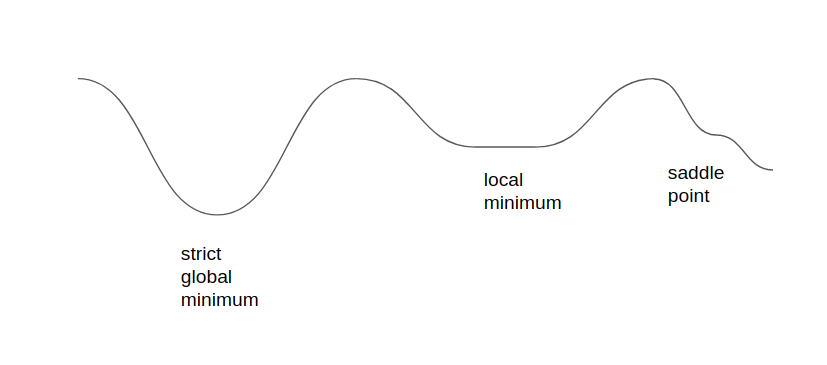
\includegraphics[width=1.0\linewidth, height=0.4\linewidth]{figures/lecture_17_non_convex_graph.png} 
\end{center}

\subsection{Local minima}

\begin{definition}[Local minimum]
A point $x^*$ is an unconstrained \textit{local minimum} if there exist $\epsilon > 0$ such that $f(x^*) \le f(x)$ for all $x$ with $\|x - x^*\| < \epsilon$.
\end{definition}

\begin{definition}[Global minimum]
A point $x^*$ is an unconstrained \textit{global minimum} if $f(x^*) \le f(x)$ for all $x$.
\end{definition}

For both definitions, we say ''strict'' if these inequalities are strict.

\begin{proposition}[Necessary Conditions for local minimum]
\propositionlabel{nc for local min}
Let $x^*$ be an unconstrained local minimum of $f\colon \R^n \to\R$ and assume $f$ is continuously differentiable ($C^1$) in an open set containing $x^*$. Then
\begin{enumerate}
    \item $\nabla f(x^*) = 0$ (First-Order Necessary Condition)
    \item If in addition $f$ is twice continuously differentiable in an open set around $x^*$, then $\nabla^2f(x^*) \succeq 0$. (Second Order Necessary Condition)
\end{enumerate}
\end{proposition}

\begin{proof}[Proof of \propositionref{nc for local min}.]
Fix any direction $d \in \R^n$.
\begin{enumerate}
    \item $g(\alpha) := f(x^* + \alpha d)$. Then
    \begin{align}
        0 &\le \lim_{\alpha \to 0} \frac{f(x^* + \alpha d) - f(x^*)}{\alpha} \label{eqn:0} \\
        &= \frac{\partial g(0)}{\partial \alpha} \nonumber \\
        &= d^\trans \nabla f(x^*) \nonumber
    \end{align}
    \ref{eqn:0} Because $x^*$ is a local minimum, $0 \le f(x^* + \alpha d) - f(x^*)$ for sufficiently small alpha. So, we can construct a sequence with only positive $\alpha$ that converges to $x^*$ such that each element $0 \le \frac{f(x^* + \alpha_n d) - f(x^*)}{\alpha_n}$ which implies that statement given that $f$ is locally differentiable.\\
    \\
    Since $d$ is arbitrary, this implies that $\nabla f(x^*) = 0$.
    \item First we represent $f(x^* + \alpha d) - f(x^*)$ using the 2nd order Taylor expansion.
    \begin{align*}
        f(x^* + \alpha d) - f(x^*) &= \alpha \nabla f(x^*)^\trans d + \frac{\alpha^2}{2}d^\trans \nabla^2 f(x^*)d + O(\alpha^2) \nonumber\\
        &= \frac{\alpha^2}{2} d^\trans \nabla^2 f(x^*) d + O(\alpha^2) \\
    \end{align*}
    Now we do the following
    \begin{align*}
        0 &\le \lim_{\alpha \to 0} \frac{f(x^* + \alpha d) - f(x^*)}{\alpha^2} \\
        &= \lim_{\alpha \to 0} \frac{1}{2}d^\trans \nabla^2 f(x^*) d + \frac{O(\alpha^2)}{\alpha^2} \\
        &= \frac{1}{2}d^\trans \nabla^2 f(x^*) d
    \end{align*}
    Because $d$ is arbitrary, this implies that $\nabla^2 f(x^*) \succeq 0$ (Positive semidefinite).
    
\end{enumerate}
\end{proof}

Note that $\nabla f(x^*) = 0$ alone does not imply $x^*$ is a local minimum. Even the necessary conditions $\nabla f(x^*) = 0$ and $\nabla^2 f(x^*) \succeq 0$ does not imply $x^*$ is a local minimum. This is because it could be that $\nabla^2 f(x^*) = 0$, but the 3rd order is not 0. For example in the 1d case, $x^* = 0$ for $f(x) = x^3$ satisfies these conditions, but is not a local minimum. Now, we will look at the actual sufficient conditions for a local minimum, but these conditions can only detect strict local minimum.

\begin{proposition}[Sufficient conditions for strict local minimum]
\propositionlabel{sufficient condition for strict local min}
    Let $f\colon \R^n \to \R$ be twice continuously differentiable ($C^2$) over an open set $S$. Suppose $x \in S$ such that $\nabla f(x^*) = 0$ and $\nabla^2f(x) \succ 0$ (positive definite). Then, $x^*$ is a strict unconstrained local minimum.
\end{proposition}

\begin{proof}[Proof of \propositionref{sufficient condition for strict local min}.]
Fix $d \in \R^n$. Note that $d^\trans \nabla^2 f(x^*) d \ge \lambda_{\text{min}} \|d\|^2$, where $\lambda_\text{min}$ is the smallest eigen value of $\nabla^2 f(x^*)$.
\begin{align}
    f(x^* + d) - f(x^*) &= \nabla f(x^*)^\trans d + \frac{1}{2}d^\trans \nabla^2 f(x^*)d + O(\|d\|^2) \label{eqn:1}\\
    &\ge \frac{\lambda_{\text{min}}}{2} \|d\|^2 + O(\|d\|^2) \nonumber \\
    &= (\frac{\lambda_{\text{min}}}{2} + \frac{O(\|d\|^2)}{\|d\|^2}) \|d\|^2 \nonumber\\
    &> 0 \label{eqn:2}
\end{align}
\ref{eqn:1} 2nd Order Taylor expansion\\
\ref{eqn:2} For sufficiently small $\|d\|$.\\ 
\\
Therefore, $x^*$ must be a strict local minimum.
\end{proof}


\subsection{Stationary Points and Gradient Descent}

For non-convex problems we must accept that gradient descent cannot always find the global minimum, but can it at least find a nearby local minimum? It turns out that for most problems we care about it can usually, but not always!

\begin{definition}[Stationary Point]
We say a point $x \in \R^n$ is a stationary point of $f\colon \R^n \to \R$ if $\nabla f(x) = 0$.
\end{definition}

\begin{proposition}
\propositionlabel{gd converges}
Gradient Descent converges to a stationary point.
\end{proposition}

\begin{proof}[Proof of \propositionref{gd converges}]
Suppose $x' = x - \eta \nabla f(x)$. From Taylor expansion we get the following
\begin{align}
    f(x') &= f(x) + \nabla f(x)^\trans (x' - x) + O(\|x' - x\|) \nonumber\\
    &= f(x) - \eta\|\nabla f(x)\|^2 + O(\eta \|\nabla f(x)\|) \nonumber \\
    &= f(x) - \eta \|\nabla f(x)\|^2 + O(\eta) \label{eqn:3}
\end{align}
\ref{eqn:3} Justified because we control $\eta$, and $\|\nabla f(x)\|$ is a constant with respect to $\eta$. \\
\\
Now we need to worry about selecting step sizes.
\subsubsection{Minimization Rule / Line Search}
Given a descent direction $d$ (example $d = - \nabla f(x)$), let our step rate $\eta$ be as follows
\[
    \eta \in \argmin_{\eta \ge 0} f(x + \eta d)
\]

Using this procedure is called \textbf{Line Search} because we search for the best step size along the direction $d$. However, exact line search can be expensive due to the argmin. \\
\\
Instead, we can approximate this minimization by using the \textbf{Armijo Rule}. 
Fix 
\[
    \gamma, s, \sigma < 1
\]
Put $\eta = \gamma^m s$ where $m$ is the smallest non-negative integer such that
\[
    f(x) - f(x + \gamma^m s d) \ge - \sigma \gamma^m s \nabla f(x)^\trans d
\]
Think of $s$ as an initial learning rate. If $s$ causes sufficient decrease then stop, otherwise keep multiplying by $\gamma$ until you do. Typical choices for parameters are 
\[
    \gamma = \frac{1}{2}, \sigma = \frac{1}{100}, s = 1
\]
\\
Notice that as long as $d$ satisfies $-\nabla f(x)^Td > 0$ that the inequality ensures that our function sequence will decrease.

\begin{proposition}
\propositionlabel{converge to stationary point}
Assume that $f$ if continuous and differentiable ($C^1$), and let $\{x_t\}$ be a sequence generated by $x_{t+1} = x_t - \eta_t \nabla f(x_t)$ where $\eta_t$ is selected by the Armijo rule. Then, every limit point of $\{x_t\}$ is a stationary point.
\end{proposition}

\begin{proof}[Proof of \propositionref{converge to stationary point}]
Let $\bar{x}$ be a limit point. By continuity $\{f(x_t)\}$ converges to $f(\bar{x})$ and therefore:
\[
    f(x_t) - f(x_{t+1}) \to 0
\]
By definition of Armijo rule:
\begin{equation}
    f(x_t) - f(x_{t+1}) \ge -\sigma \eta_t \|\nabla f(x_t)\|^2 \label{eqn:4}
\end{equation}
Suppose for the sake of contradiction that $\bar{x}$ is not a stationary point of $f$. Then,
\[
    \limsup_{t \to \infty} -\|\nabla f(x_t)\|^2 < 0
\]
By \ref{eqn:4}, this must mean that $\eta_t \to 0$. This implies $\exists t_0$ such that $\forall t \ge t_0$
\[
    f(x_t) - f(x_t - \frac{\eta_t}{\gamma} \nabla f(x_t)) < \frac{\sigma \eta_t}{\gamma} \|\nabla f(x_t)\|^2
\]
Because $\eta_t \to 0$, we know that after some $t_0$ all step sizes are chosen with a $m\ge 1$. Therefore, going back one iteration of Armijo rule was not good enough to satisfy the inequality or else that or some previous step size would have been chosen. \\
\\
Now let $\tilde{\eta_t} = \frac{\eta_t}{\gamma}$ and we can continue as follows
\begin{align}
    \frac{f(x_t) - f(x_t - \tilde{\eta_t} \nabla f(x_t))}{\tilde{\eta_t}} &< \sigma \|\nabla f(x)\|^2 &\Rightarrow \nonumber \\
    \nabla f(x_t - \tilde{\eta_t} \nabla f(x_t))^T \nabla f(x_t) &< \sigma \|\nabla f(x)\|^2 &\Rightarrow \label{eqn:5} \\
    \|\nabla f(x_t) \|^2 &\le \sigma \|\nabla f(x_t) \|^2 & \label{eqn:6}
\end{align}
\\
\ref{eqn:5} using Mean Value Theorem (MVT) \\
\ref{eqn:6} by taking the limit as $\eta_t \to 0 \Rightarrow \tilde{\eta_t} \to 0$ \\
\\
This is a contradiction because $0 < \sigma < 1$. Therefore, the limit point $\bar{x}$ is a stationary point of $f$.
\end{proof}
Therefore, if we can use the Armijo rule to determine step sizes that guarantee that gradient descent will converge to a stationary point.
\end{proof}

\subsection{Saddle Points}

Now that we have found that gradient descent will converge to a stationary point, how concerned should we be that the stationary point is not a local minimum?

\begin{definition}[Saddle points]
Saddle points are stationary points that are not local optimum.
\end{definition}
This means that if $f$ is twice differentiable then $\nabla^2 f(x)$ has both positive and negative eigenvalues.
\subsubsection{How do saddle points arise?}
In most non-convex problems there exists several local minima. This is clear to see in problems that have natural symmetry such as in a two layer fully connected neural networks. 
\begin{center}
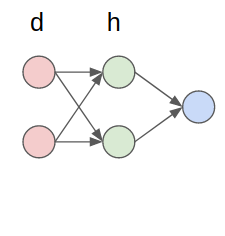
\includegraphics[width=0.3\linewidth, height=0.3\linewidth]{figures/lecture_17_neural_network.png} 
\end{center}
Notice that any permutation of the units of the hidden layer would preserve the same function, so we have approximately $h!$ local minima. Typically a convex combination of two distinct local minimum in a non-convex problem is not a local minimum. In the case where $\nabla f(x)$ is differentiable, then by MVT we know that there must exist another stationary point between any two local minimum, so often there exists at least one saddle point between any two distinct local minimum. Hence, many local minimum tends to lead to many saddle points. \\
\\
However, recent work has demonstrated that saddle points are usually not a problem.
\begin{enumerate}
    \item The set of saddle points form a measure zero set for random initialization. \cite{DBLP:journals/corr/GeHJY15}
    \item Saddle points can be avoided with noise addition. \cite{DBLP:journals/corr/abs-1710-07406}
\end{enumerate}
\printbibliography

\section{Escaping saddle points} 

This lecture formalizes and shows the following intuitive statement for
nonconvex optimization:
\begin{center}
	\textbf{Gradient descent almost never converges to (strict) saddle points.}
\end{center}
The result was shown in~\cite{lee2016gradient}. Let's start with some definitions.

\begin{definition}[Stationary point]
We call $x^*$ a stationary point if the gradient vanishes at $x^*,$ i.e., 
$\nabla f(x^*) = 0$. 
\end{definition}

We can further classify stationary points into different categories. One
important category are saddle points.

\begin{definition}[Saddle point]
A stationary point $x^*$ is a \emph{saddle point} 
if for all $\epsilon>0$,  there are points $x,y \in B(x^*;\epsilon)$ 
s.t.~$f(x)\leq f(x^*)\leq f(y)$.
\end{definition}

\begin{definition}[Strict saddle point]
For a twice continuously differentiable function $f\in C^2$, a saddle point
$x^*$ is a \emph{strict saddle point} if the Hessian at that point is not
positive semidefinite, i.e.  $\lambda_{\text{min}}(\nabla^2 f(x^*)) < 0$, where
$\lambda_{\text{min}}$ denotes the smallest eigenvalue.
\end{definition}

\subsection{Dynamical systems perspective}

It'll be helpful to think of the trajectory defined by gradient descent as a
dynamical system.
To do so, we view each gradient descent update as a operator.  
For a fixed step size $\eta$, let
$$
g(x) = x-\eta\nabla f(x)
$$ 
so the notation for the result of iteration $t$ from our previous discussion of gradient descent carries over as $x_t = g^t(x_0) = g(g(...g(x_0)))$, where $g$ is applied $t$ times on the initial point $x_0$. We call $g$ the gradient map. Note that $x^*$ is stationary iff. it is a fixed point of the gradient map i.e. $g(x^*) = x^*$. Also note that
$D g(x) = I - \eta\nabla^2 f(x)$ (Jacobian of $g$) , a fact that will become important later. Now we formalize a notion of the set of "attractors`` of $x^*$.
\begin{definition}
The global stable set of $x^*$, is defined as
$$
W^S(x^*) = \{ x\in\R^n: \lim_{t} g^t(x) = x^* \}
$$
In words, this is the set of points that will eventually converge to $x^*$.
\end{definition}

With this definition out of the way, we can state the main claim formally as
follows.

\begin{theorem}
\theoremlabel{lecture18-main}
Assume $f\in C^2$ and is $\beta$-smooth. Also assume that the step size $\eta <
1/\beta$. Then for all strict saddle points $x^*$, its set of attractors
$W^S(x^*)$ has Lebesgue measure $0$.
\end{theorem}

\begin{remark}
In fact, it could be proven with additional technicalities that the Lebesgue measure of 
$
\bigcup_{\text{strict saddle points }x^*} W^S(x^*)
$
is also 0. This is just another way to say that gradient descent almost surely converges to local minima. 
\end{remark}

\begin{remark}
By definition, this also holds true to any probability measure absolutely continuous w.r.t. the Lebesgue measure (e.g. any continuous probability distribution). That is,
$$\mathbb{P}(\lim_t x_t = x^*) = 0$$
\end{remark}

However, the theorem above is only an asymptotic statement. Non-asymptotically, even with fairly natural random initialization schemes and non-pathological functions, gradient descent can be significantly slowed down by saddle points. 
The most recent result \cite{du2017gradient} is that gradient descent takes exponential time to escape saddle points (even though the theorem above says that they do escape eventually). We won't prove this result in this lecture.

\subsection{The case of quadratics}
Before the proof, let's go over two examples that will make the proof more intuitive:

\begin{example}
$f(x) = \frac{1}{2} x^THx$ where $H$ is an $n$-by-$n$ matrix, symmetric but not positive semidefinite. 
For convenience, assume $0$ is not an eigenvalue of $H$.
So $0$ is the only stationary point and the only strict saddle point for this problem.

We can calculate
$g(x) = x - \eta Hx = (I-\eta H)x$ and 
$g^t(x) = (I-\eta H)^tx$. 
And we know that 
$\lambda_i(I - \eta H) = 
1-\eta \lambda_i(H)$, where $\lambda_i$ for $i=1...n$ could denote any one of the eigenvalues.
So in order for $\lim_t g^t(x) = \lim_t (1-\eta \lambda_i(H))^t x$ to converge to 0, we just need $\lim_t (1-\eta \lambda_i(H))^t$ to converge to 0, that is, $|1-\eta \lambda_i(H)| < 1$. This implies that
$$W^S(0) = \text{span}\bigg\{ u| Hu=\lambda u,  0< \lambda < \frac{\eta}{2} \bigg\}$$
i.e. the set of eigenvectors for the positive eigenvalues smaller than 
$\frac{\eta}{2}$. Since $\eta$ can be arbitrarily large, we just consider the larger set of eigenvectors for the positive eigenvalues. By our assumption on $H$, this set has dimension lower than $n$, thus has measure 0.
\end{example}

\begin{example}
Consider the function 
$f(x,y) = \frac{1}{2}x^2 + \frac{1}{4}y^4 - \frac{1}{2}y^2$  with corresponding
gradient update 
\[
g(x,y) = 
\begin{bmatrix}
(1-\eta)x\\
(1+\eta)y - \eta y^3 
\end{bmatrix}\,,
\]
and Hessian
\[
\nabla^2 f(x,y) = 
 \begin{bmatrix}
1 & 0 \\
0 & 3y^2-1 \\
\end{bmatrix}\,.
\]
We can see that $(0,-1)$ and $(0,1)$ are the local minima, and $(0,0)$ is the only strict saddle point. Similar to in the previous example, $W^S(0)$ is a low-dimensional subspace. 

\subsection{The general case}

We conclude this lecture with a proof of the main theorem.

\begin{proof}[Proof of \theoremref{lecture18-main}]
First define the local stable set of $x^*$ as
$$
W^S_\epsilon(x^*) 
= \{ x\in B(x^*;\epsilon): g^t(x)\in B(x^*;\epsilon) ~\forall t \}
$$
Intuitively, this describes the subset of $B(x^*;\epsilon)$ that stays in $B(x^*;\epsilon)$ under arbitrarily many gradient maps. This establishes a notion of locality that matters for gradient descent convergence, instead of $B(x^*;\epsilon)$ which has positive measure.

Now we state a simplified version of the stable manifold theorem without proof: For a diffeomorphism $g:\R^n\rightarrow\R^n$, if $x^*$ is a fixed point of $g$, then for all $\epsilon$ small enough, $W^S_\epsilon(x^*)$ is a submanifold of dimension equal to the number of eigenvalues of the $Dg(x^*)$ that are $\leq 1$. A diffeomorphism, roughly speaking, is a differentiable isomorphism. In fact, since differentiability is assumed for $g$, we will focus on the isomorphism.

Let $x^*$ be a strict saddle point.
Once we have proven the fact that $g$ is a diffeomorphism (using the assumption that $\eta<1/\beta$), we can apply the stable manifold theorem since $x^*$ is a fixed point of $g$. 
Because $\nabla^f (x^*)$ must have an eigenvalue $<0$, $Dg$ must have an eigenvalue $>1$, so 
the dimension of $W^S_\epsilon(x^*)$ is less than $n$ and $W^S_\epsilon(x^*)$ has measure 0. 

If $g^t(x)$ converges $x^*$, there must $\exists T$ large enough s.t. $g^T(x)\in W_\epsilon^S(x^*)$. 
So $W^S(x^*)\subseteq \bigcup_{t\geq 0 }g^{-t}(W_\epsilon^S(x^*))$.
For each $t$, $g^t$ is in particular an isomorphism (as a composition of isomorphisms), and so it $g^{-t}$.
Therefore $g^{-t}(W_\epsilon^S(x^*))$ has the same cardinality as 
$W_\epsilon^S(x^*)$ and has measure 0. Because the union is over a countable set, the union also has measure 0, thus its subset $W^S(x^*)$ ends up with measure 0 and we have the desired result.

Finally we show that $g$ is bijective to establish the isomorphism (since it is assumed to be smooth). It is injective because, assuming $g(x) = g(y)$, by smoothness,
$$
\|x-y\| = \|g(x) + \eta\nabla f(x) - g(y) - \eta\nabla f(x) \|
 = \eta\|\nabla f(x) - \nabla f(y)\|\leq \eta\beta\|x-y\|
$$
Because $\eta\beta < 1$, we must have $\|x-y\|=0$.
To prove that $g$ is surjective, we construct an inverse function
$$h(y) = \argmin_x \frac{1}{2}\|x-y\|^2 - \eta f(x)$$
a.k.a. the proximal update. For $\eta < 1/\beta$, $h$ is strongly convex, and by the KKT condition,
$y = h(y) - \nabla f(h(y)) = g(h(y))$. This completes the proof.
\end{proof}

\end{example}

\section{Lecture 19: Alternating minimization and EM}

This lecture was a sequence of code examples that you can find here:

\begin{center}
{\Large
\href{https://ee227c.github.io/code/lecture19.html}{Lecture 19}
}

(opens in your browser)
\end{center}



\section{Lecture 20: Derivative-free optimization, policy gradient, controls}

This lecture was a sequence of code examples that you can find here:

\begin{center}
{\Large
\href{https://ee227c.github.io/code/lecture20.html}{Lecture 20}
}

(opens in your browser)
\end{center}



\section{Lecture 21: Non-convex constraints part 1}
Recall that convex minimization refers to minimizing convex functions over convex constraints. Today we will begin to explore minimizing convex functions with non-convex constraints. It is difficult to analyze the impact of ``non-convexity" in general, since that can refer to anything that is not convex, which is a very broad class of problems. So instead, we will focus on solving least squares with sparsity constraints:
\begin{align*}
    \min_{\|x\|_0 \leq s} \|Ax-y\|^2_2
\end{align*}
for $y \in \mathbb{R}^{n}$, $A \in \mathbb{R}^{n \times d}$, and $x \in \mathbb{R}^{d}$ where $d < n$. We will show that in general even this problem is hard to solve but that for a restricted class of problems there is an efficient convex relaxation.

Least squares with sparsity constraints can be applied to solving compressed sensing and sparse linear regression, which are important in a variety of domains. In compressed sensing, $A$ is a measurement model and $y$ are the measurements of some sparse signal $x$. Compressed sensing is applied to reduce the number of measurements needed for, say, an MRI because by including a sparsity constraint on $x$ we are able to recover the signal $x$ in fewer measurements.

In sparse linear regression, $A$ is the data matrix and $y$ is some outcome variable. The goal of sparse linear regression is to recover a weights $x$ on a sparse set of features that are responsible for the outcome variable. In genetics, $A$ could be the genes of a patient, and $y$ is whether they have a particular disease. Then the goal is to recover a weights $x$ on a sparse set of genes that are predictive of having the disease or not.

When there is no noise in the linear equations, we can simplify the problem to
\begin{align*}
    & \min \|x\|_0 \\
    &  Ax = y
\end{align*}

\subsection{Hardness}
Even this simplification is NP-hard, as we will show with a reduction to exact 3-cover, which is NP-complete. Our proof is from \cite{foucart2013mathematical}.
\begin{definition}
The \textit{exact cover by 3-sets} problem is given a collection $\{T_i\}$ of 3-element subsets of $[n]$, does there exist an exact cover of $[n]$, a set $z \subseteq [d]$ such that $\cup_{j \in z} T_j = [n]$ and $T_i \cap T_j = \emptyset$ for $j \neq j' \in z$?
\end{definition}

\begin{definition}
The support of a vector $x$ is defined as
\begin{align*}
\text{supp}(x) = \{i \mid x_i \neq 0 \}.
\end{align*}
\end{definition}

\begin{theorem}
$l_0$-minimization for general $A$ and $y$ is NP-hard.
\end{theorem}
\begin{proof}
Define matrix $A$ as
\begin{align*}
    A_{ij} = \begin{cases}
    1 & \text{if } i \in T_j \\
    0 & \text{o.w}
    \end{cases}
\end{align*}

and $y$ as the all ones vector. Note that from our construction we have $\|Ax\|_0 \leq 3\|x\|_0$, since each column of $A$ has 3 non-zeros. If $x$ satisfies $Ax = y$, we thus have $\|x\|_0 \geq \frac{\|y\|_0}{3} = \frac{n}{3}$. Let us now run $l_0$-minimization on $A, y$ and let $\hat{x}$ be the output. There are two cases

\begin{enumerate}
    \item If $\|\hat{x}\|_0 = \frac{n}{3}$, then $y = \text{supp}(\hat{x})$ is an exact 3-cover. % define supp
    \item If $\| \hat{x}\|_0 > \frac{n}{3}$, then no exact 3-sover can exist because it would achieve $\|\hat{x}\|_0 = \frac{n}{3}$ and hence violate optimality of the solution derived through $l_0$ minimization.
\end{enumerate}

Thus, since we can solve exact 3-cover through $l_0$ minimization, $l_0$ minimization must also be NP-hard.
\end{proof}

\subsection{Convex relaxation}
Although $l_0$-minimization is NP-hard in general, we will prove that for a restricted class of $A$, we can relax $l_0$-minimization to $l_1$-minimization. First, define the set of approximately sparse vectors with support $S$ as those whose $l_1$ mass is dominated by $S$. Formally,
\begin{definition}
The set of approximately sparse vectors with support $S$ is
\begin{align*}
    C(S) = \{ \Delta \in \mathbb{R}^{d} \mid \|\Delta_{\bar{S}}\|_1 \leq \|\Delta_S \|_1 \}
\end{align*}
where $\bar{S} = [d] / S$ and $\Delta_s$ is $\Delta$ restricted to $S$,
\begin{align*}
    (\Delta_{S})_i = \begin{cases}
        \Delta_i & \text{if } i \in S \\
        0 & \text{o.w}
    \end{cases}
\end{align*}
\end{definition}
Recall that the nullspace of matrix $A$ is the set $\text{null} (A) = \{ \Delta \in \mathbb{R}^{d} \mid A\Delta = 0 \}$. The nullspace is the set of "bad" vectors in our estimation problem. Consider a solution $Ax = y$. If $\Delta \in \text{null(A)}$, then $x + \Delta$ is also a solution since $A(x + \Delta) = Ax + A\Delta = Ax = b$. Thus, we focus on matrices whose nullspace only contains zero on the set of sparse vectors that we care about.
\begin{definition}
The matrix $A$ satisfies the restricted nullspace property (RNP) with respect to the support $S$ if $C(S) \cup \text{null}(A) = \{ 0 \}$.
\end{definition}
With these definitions in place, we can now state our main theorem.
\begin{theorem}
Given $A \in \R^{n \times d}$ and $y \in \R^n$ we consider the solution to the $l_0$-minimization problem $x^* = \argmin_{Ax=y}\|x\|_0$. Assume $x^*$ has support $S$ and let the matrix $A$ satisfy the restricted nullspace property with respect to S. Then given the solutions of the $l_1$-minimization problem $\hat{x} = \argmin_{Ax=y}\|x\|_1$ we have $\hat{x} = x^*$.
\end{theorem}

\begin{proof}
We first note that by definition both $x^*$ and $\hat{x}$ satisfy our feasibility constraint $Ax=y$. Letting $\Delta = \hat{x} - x^*$ be the error vector we have $A\Delta = A\hat{x} - Ax^* = 0$, which implies that $\Delta \in null(A)$.

Our goal now is to show that $\Delta \in C(S)$ then we would have $\Delta = 0$ from the restricted nullspace property. First, since $\hat{x}$ is optimal in $l_1$ it follows that $\|\hat{x}\|_1 \le \|x^*\|_1$. We then have
\begin{align*}
    \|x_S^*\|_1 &= \|x^*\|_1 \ge \|\hat{x}\|_1\\
                &= \|x^* + \Delta\|_1\\
                &= \|x_S^* + \Delta_S\|_1 + \|x_{\overline{S}}^* + \Delta_{\overline{S}}\|_1 &&\text{by splitting the $l_1$ norm,}\\                            
                &= \|x_S^* + \Delta_S\|_1 + \|\Delta_{\overline{S}}\|_1 &&\text{by the support assumption of $\|x^*\|_1$,}\\
                &\ge \|x_S^*\|_1 - \|\Delta_S\|_1 + \|\Delta_{\overline{S}}\|_1.
\end{align*}
Hence $\|\Delta_S\|_1 \ge \|\Delta_{\overline{S}}\|_1$, which implies $\Delta \in C(S)$.
\end{proof}

So far, so good. We have shown that the $l_1$-relaxation works for certain matrices. A natural question however is what kinds of matrices satisfy the restricted nullspace property. In order to get a handle on this, we will study yet another nice property of matrices, the so called restricted isometry property (RIP). Later, we will then see that specific matrix ensembles satisfy RIP with high probability.
\begin{definition}
A matrix $A$ satisfies the $(s, \delta)$-RIP if for all $s$-sparse vectors $x$ ($\|x\|_0 \le s$), we have
\[
(1 - \delta)\|x\|_2^2 \le \|Ax\|_2^2 \le (1 + \delta) \|x\|_2^2.
\]
\end{definition}
The intuition is that $A$ acts like an isometry on sparse vectors (a true isometry would have $\delta = 0$). The RIP is useful since it implies that the difference between two $s$-sparse vectors cannot be mapped to $0$. By looking at the singular values of $A$ we can derive the following lemma.
\begin{lemma}
\label{RIPlemma}
If $A$ has $(s, \delta)$-RIP, then
\[
\|A_S^{\trans}A_S - I_S\|_2 \le \delta
\]
for all subsets $S$ of size $s$. Where

\begin{align*}
    (A_S)_{ij} = \begin{cases}
    A_{ij} & \text{if } j \in S \\
    0 & \text{o.w}.
    \end{cases}
\end{align*}
\end{lemma}
We now show that the RIP implies the restricted nullspace property. 
\begin{theorem}
If the matrix $A$ has the $(2s, \delta)$-RIP, then it also has the restricted nullspace property for all subsets $S$ of cardinality $|S| \le s$.
\end{theorem}
\begin{proof}
Let $x \in null(A)$ be arbitrary but not equal to $0$. Then we have to show that $x \not\in C(S)$ for any $S$ with $|S| \le s$. In particular, let $S_0$ be the set indices of the $s$ largest coefficients in $x$. It suffices to show that $\|x_{S_0}\|_1 <  \|x_{\overline{S}_0}\|_1$ since it would then hold for any other subset.

We write
\[
\overline{S}_0 = \bigcup\limits_{j = 1}^{\lceil \frac{d}{s} \rceil - 1} S_j
\]
where 
\begin{itemize}
\item $S_1$ is the subset of indices corresponding to the $s$ largest entries in $\overline{S}_0$
\item $S_2$ is the subset of indices corresponding to the $s$ largest entries in $\overline{S}_0\setminus S_1$
\item $S_3$ is the subset of indices corresponding to the $s$ largest entries in $\overline{S}_0\setminus S_1 \setminus S_2$
\item etc\ldots
\end{itemize}
So we have $x = x_{S_0} + \sum\limits_j x_{S_j}$. We have decomposed $x$ into blocks of size $s$. This is sometimes called shelling. From RIP, we have
\[
\|x_{S_0}\|_2^2 \le \frac{1}{1 - \delta}\|Ax_{S_0}\|_2^2.
\]
Since $x \in null(A)$ by assumption we have
\begin{align*}
&A(x_{S_0} + \sum\limits_{j \ge 1} x_{S_j}) = 0\\
\implies&Ax_{S_0} = -\sum\limits_{j \ge 1} Ax_{S_j}.
\end{align*}
Hence
\begin{align*}
\|x_{S_0}\|_2^2 &\le \frac{1}{1 - \delta}\|Ax_{S_0}\|_2^2\\
                &= \frac{1}{1 - \delta}\langle Ax_{S_0}, Ax_{S_0}\rangle\\
                &= \frac{1}{1 - \delta}\sum\limits_{j \ge 1}\langle Ax_{S_0}, Ax_{S_j}\rangle\\
                &= \frac{1}{1 - \delta}\sum\limits_{j \ge 1}\langle Ax_{S_0}, -Ax_{S_j}\rangle\\
                &=  \frac{1}{1 - \delta}\sum\limits_{j \ge 1}(\langle Ax_{S_0}, -Ax_{S_j}\rangle - \langle x_{S_0}, x_{S_j} \rangle) && \text{since $\langle x_{S_0}, x_{S_j} \rangle = 0$}\\                
                &=  \frac{1}{1 - \delta}\sum\limits_{j \ge 1}\langle x_{S_0}, (I - A^{\trans}A)x_{S_j}\rangle\\                
                &\le \frac{1}{1 - \delta}\sum\limits_{j \ge 1}\|x_{S_0}\|_2 \delta \|x_{S_j}\|_2 && \text{from Lemma~\ref{RIPlemma}}.
\end{align*}
So we have
\begin{align}
\|x_{S_0}\|_2 \le \frac{\delta}{1 - \delta}\sum\limits_{j \ge 1}\|x_{S_j}\|_2.\equationlabel{l2norm}
\end{align}
By construction, for each $j \ge 1$, we have
\[
\|x_{s_j}\|_\infty \le \frac{1}{S}\|X_{S_{j-1}}\|_1
\]
and hence
\[
\|x_{s_j}\|_2 \le \frac{1}{\sqrt{S}}\|X_{S_{j-1}}\|_1.
\]
Plugging into \equationref{l2norm}, we get
\begin{align*}
\|x_{S_0}\|_1 &\le \sqrt{S}\|x_{S_0}\|_2\\
              &\le \frac{\sqrt{S}\delta}{1 - \delta}\sum\limits_{j \ge 1}\|x_{S_j}\|_2\\
              &\le \frac{\delta}{1 - \delta}\sum\limits_{j \ge 1}\|x_{S_{j-1}}\|_1\\
              &\le \frac{\delta}{1 - \delta}(\|x_{s_0}\|_1 + \sum\limits_{j \ge 1}\|x_{S_{j-1}}\|_1)
\end{align*}
which is equivalent to
\[
\|x_{s_0}\|_1 \le \frac{\delta}{1 - \delta}(\|x_{s_0}\|_1 + \|x_{\overline{s}_0}\|_1).
\]
Simple algebra gives us $\|x_{s_0}\|_1 \le \|x_{\overline{s}_0}\|_1$ as long as $\delta < \frac{1}{3}$.
\end{proof}
Now that we've shown that if $A$ has the RIP then $l_1$-relaxation will work, we look at a few examples of naturally occurring matrices with this property.
\begin{theorem}
Let $A \in \R^{n \times d}$ be defined as $a_{ij} \sim \mathcal{N}(0,1)$ iid. Then the matrix $\frac{1}{\sqrt{n}}A$ has $(s, \delta)$-RIP for $n$ at least $\mathcal{O}\left(\frac{1}{\delta^2}s \log{\frac{d}{s}}\right)$.
\end{theorem}
The same holds for sub-Gaussians. We have similar results for more structured matrices such as subsampled Fourier matrices.
\begin{theorem}
Let $A \in \R^{n \times d}$ be a subsampled Fourier matrix. Then $A$ has $(s, \delta)$-RIP for $n$ at least $\mathcal{O}\left(\frac{1}{\delta^2}s \log^2 s\log d\right)$.
\end{theorem}
This result is from \cite{DBLP:journals/corr/HavivR15a} using work from \cite{doi:10.1002/cpa.20227, Bourgain2014, DBLP:journals/tit/CandesT06}. $\mathcal{O}\left(\frac{1}{\delta^2}s\log d\right)$ is conjectured but open.

There is a lot more work on convex relaxations. For sparsity alone people have studied many variations e.g.
\begin{itemize}
    \item \textbf{Basic pursuit denoising (BPDN)} $\min \|x\|_1$ such that $\|Ax - y \|_2 \le \epsilon$
    \item \textbf{Constrained LASSO} $\min \|Ax - y\|_2^2$ such that $\|x\|_1 \le \lambda$
    \item \textbf{Lagrangian LASSO} $\min \|Ax - y\|_2^2 + \lambda \|x\|_1$
\end{itemize}
There are also convex relaxations for other constraints. For example $\min rank(X)$ such that $A(X)=Y$ is hard, a simpler problem is to solve the nuclear norm minimization instead: $\min \|X\|_*$ such that $A(X)=Y$. This can be applied to low-rank estimation for images or matrix completion.

\section{List of contributors}
\sectionlabel{contributors}

Many thanks to the students of EE227C for their generous help in creating these
lecture notes.

\begin{description}
\item[Lecture 2:] Michael Cheng, Neil Thomas, Morris Yau
\item[Lecture 3:]
\item[Lecture 5:] Victoria Cheng, Kun Qian, Zeshi Zheng
\item[Lecture 6:] Adam Gleave, Andy Deng, Mathilde Badoual
\item[Lecture 7:] Aurelien Bibaut, Zhi Chen, Michael Zhang
\item[Lecture 8:] Eugene Vinitsky
\item[Lecture 9:] John Miller, Vlad Feinburg
\item[Lecture 12:] Erin Grant
\item[Lecture 14:] Feynman Liang
\item[Lecture 15:] Lydia Liu, Tijana Zrnic
\item[Lecture 17:] Adam Villaflor
\item[Lecture 18:] Yu Sun
\item[Lecture 21:] Smitha Milli, Karl Krauth
\item[Lecture 23:] Soroush Nasiriany, Armin Askari
\end{description}

\section{Acknowledgments}

These notes build on an earlier course by Ben Recht, as well as an upcoming
textbook by Recht and Wright. Some chapters also closely follow Bubeck's
monograph on the topic~\cite{Bubeck}.


\bibliographystyle{alpha}
\bibliography{notes}

\end{document}
